\section{Evaluation}~\label{sec:evaluation}

In this section, we empirically evaluate our techniques against other \pr clause
learning techniques. In doing so, we aim to answer the following research questions:


\begin{enumerate}
    \item Can our approach provide short \pr proofs for certain benchmark families?
    \item Is our approach less sensitive to encoding choices compared to other
    \pr learning techniques?
    % \item Can these techniques underperform or outperform SAT solvers on other certain benchmark
    % families?
\end{enumerate}


We compare to the two main tools for learning \pr clauses are \sadical (based on SDCL)
and \prelearn (a preprocessing technique that calls \sadical). To be consistent with our approach,
we run \prelearn with 50 iterations and for 30 seconds. We also compare to \cadical, as a baseline with no \pr clause learning.

In \autoref{subsec:eval-pigeonhole}, we compare all approaches
on the pigeonhole principle. We evaluate based on time taken, the length of
the proof, and the sensitivity to the encoding of the formula. 

In \autoref{subsec:eval-satcomp}, we evaluate the solvers on benchmarks from the
annual '22, '23, and '24 SAT competition's main
tracks~\cite{satcomp2022,satcomp2023,satcomp2024}.

In \autoref{subsec:eval-discussion}, we highlight certain benchmark families
that benefit from \pr clause learning. We evaluate the different approaches on these families.


Finally, we analyze the use of specific heuristic choices in \tool
by turning heuristics off individually and observing their effect (\autoref{subsec:eval-heuristics}). 

All experiments were performed in the Anvil Supercomputing Center on nodes with
128 cores and 2 GB RAM per core~\cite{anvil}. We ran 64 experiments in parallel per node
with a 5,000 second timeout, the default timeout for the SAT competition.

\subsection{Pigeonhole results}~\label{subsec:eval-pigeonhole}

\begin{figure*}[!t]
    \centering
    \begin{subfigure}[t]{0.4\textwidth}
        \centering
        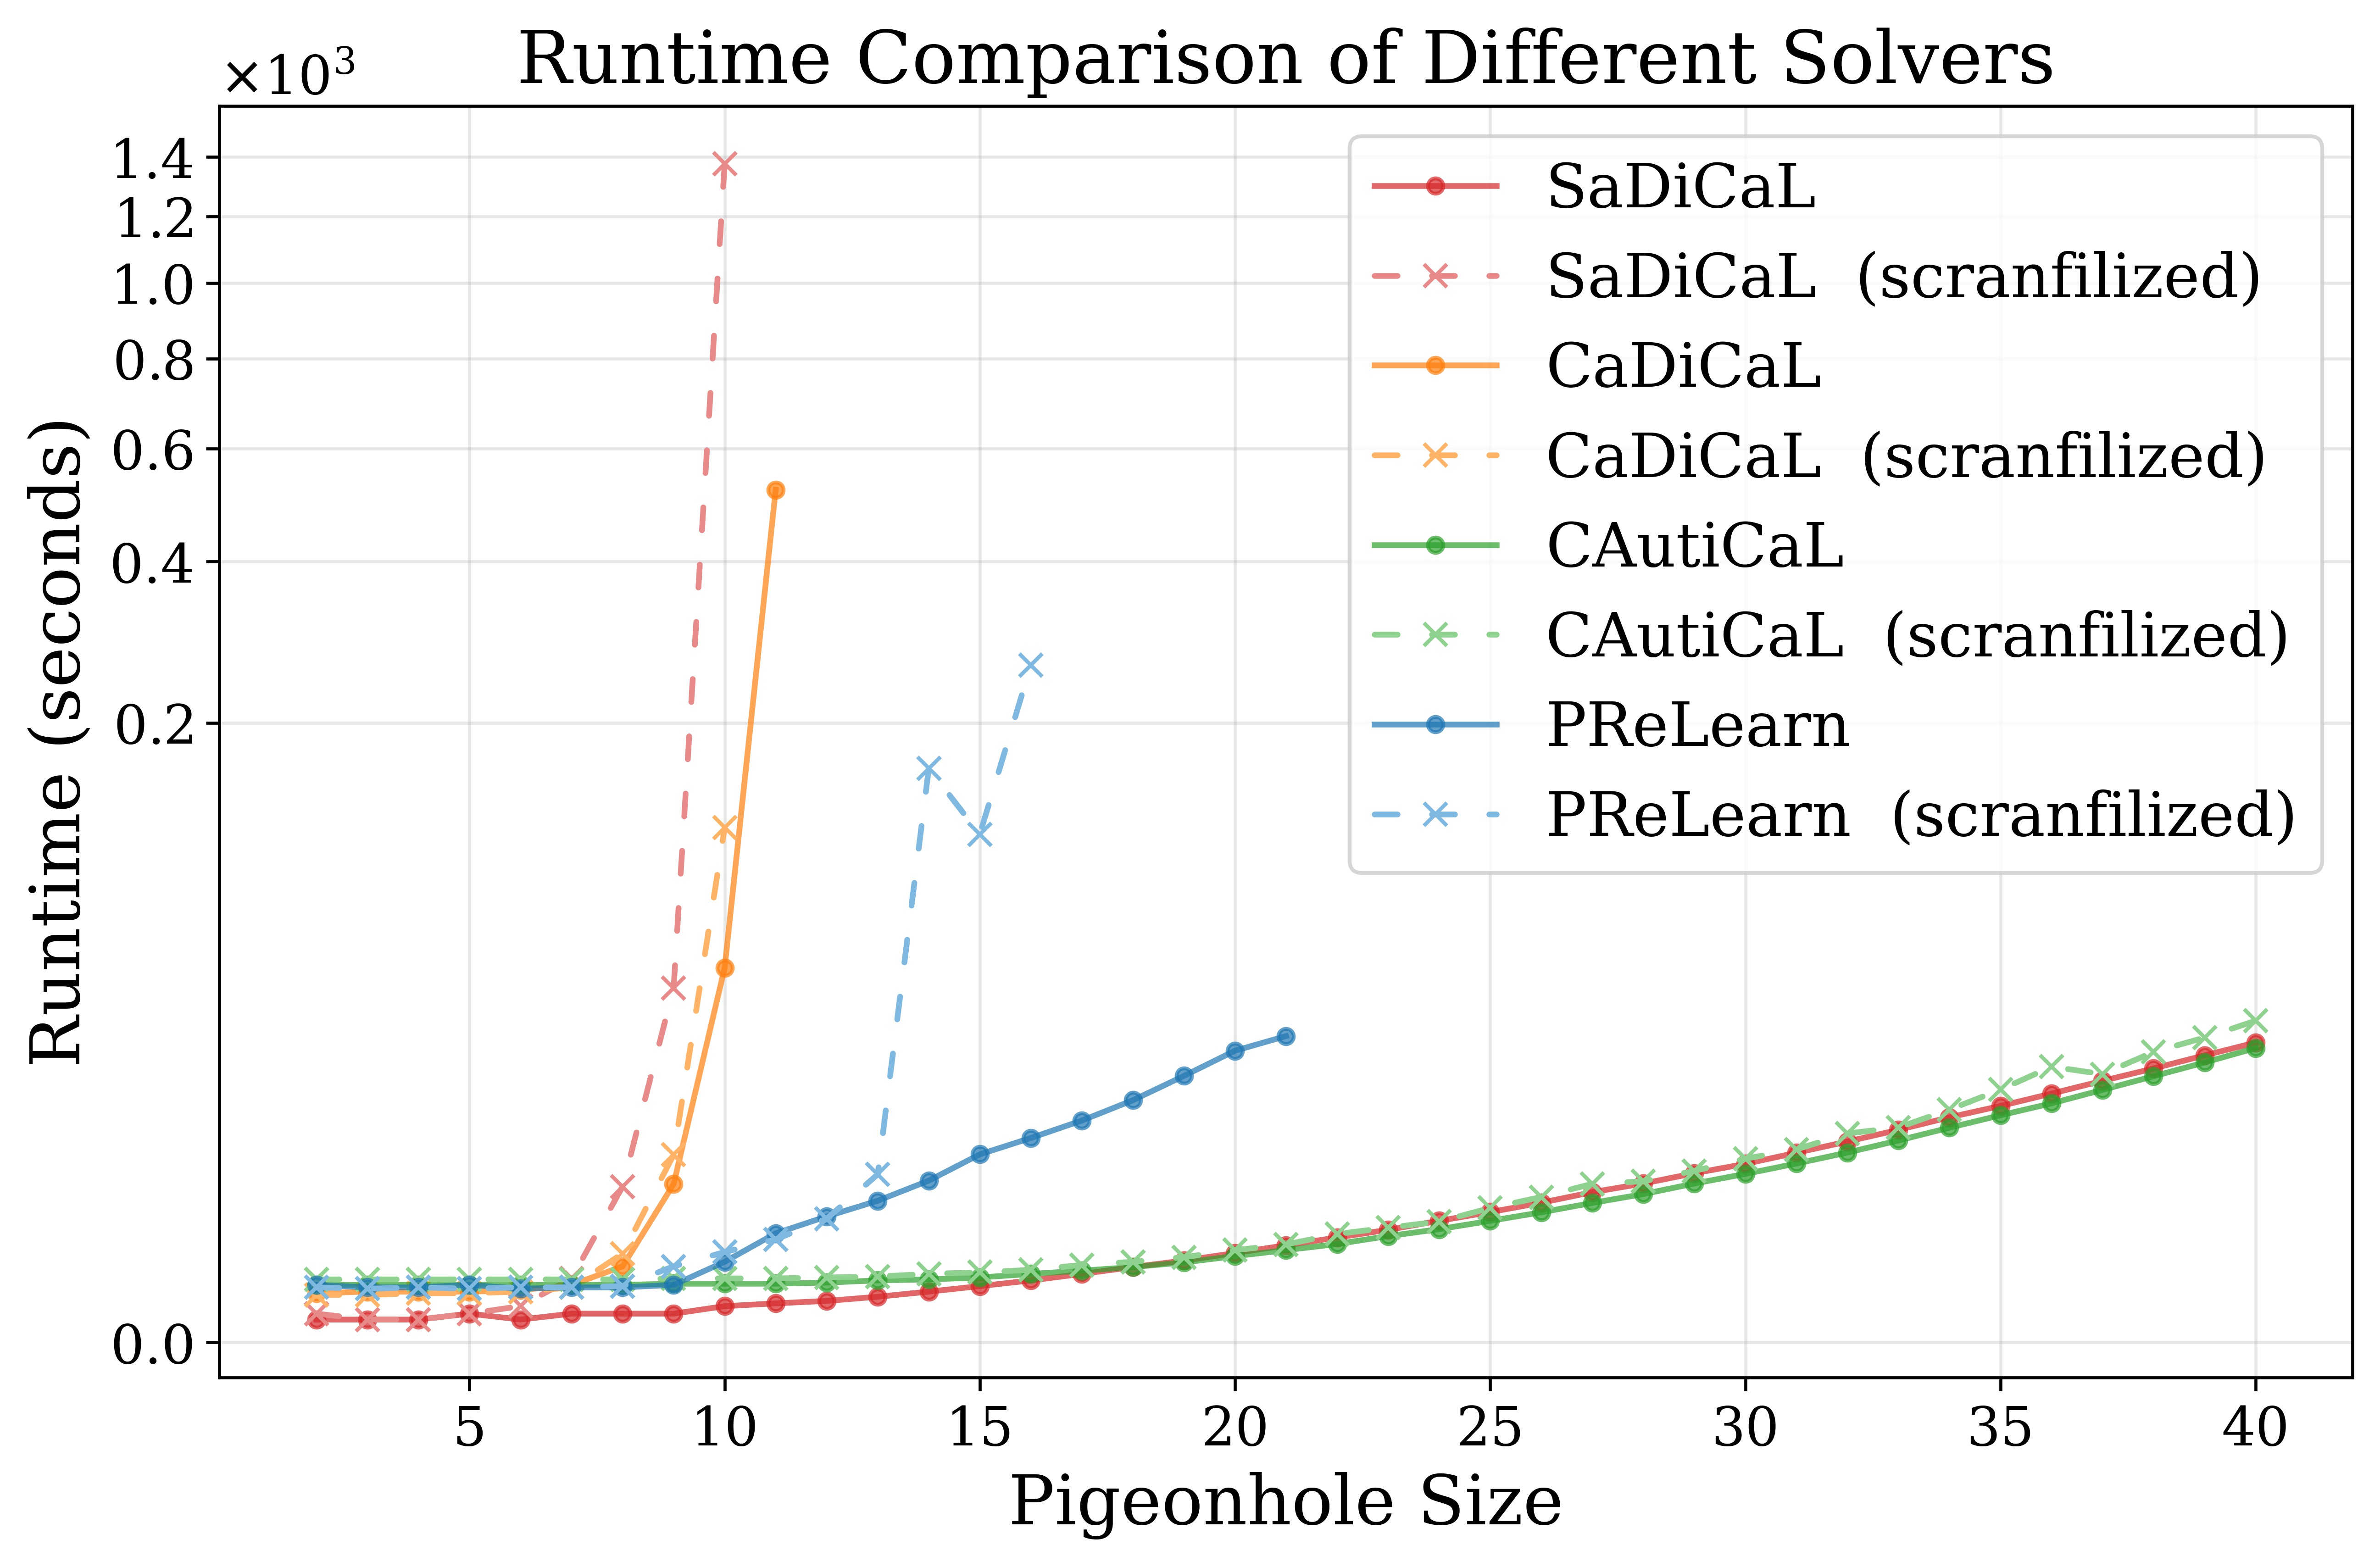
\includegraphics[width=\textwidth]{figs/pigeonhole_runtime_comparison.jpg}
        % \caption{Runtime on Pigeonhole Principle Formulas}
        \label{fig:pigeonhole-runtime-comparison}
    \end{subfigure}
    \hspace{0.06\textwidth}
    \begin{subfigure}[t]{0.4\textwidth}
        \centering
        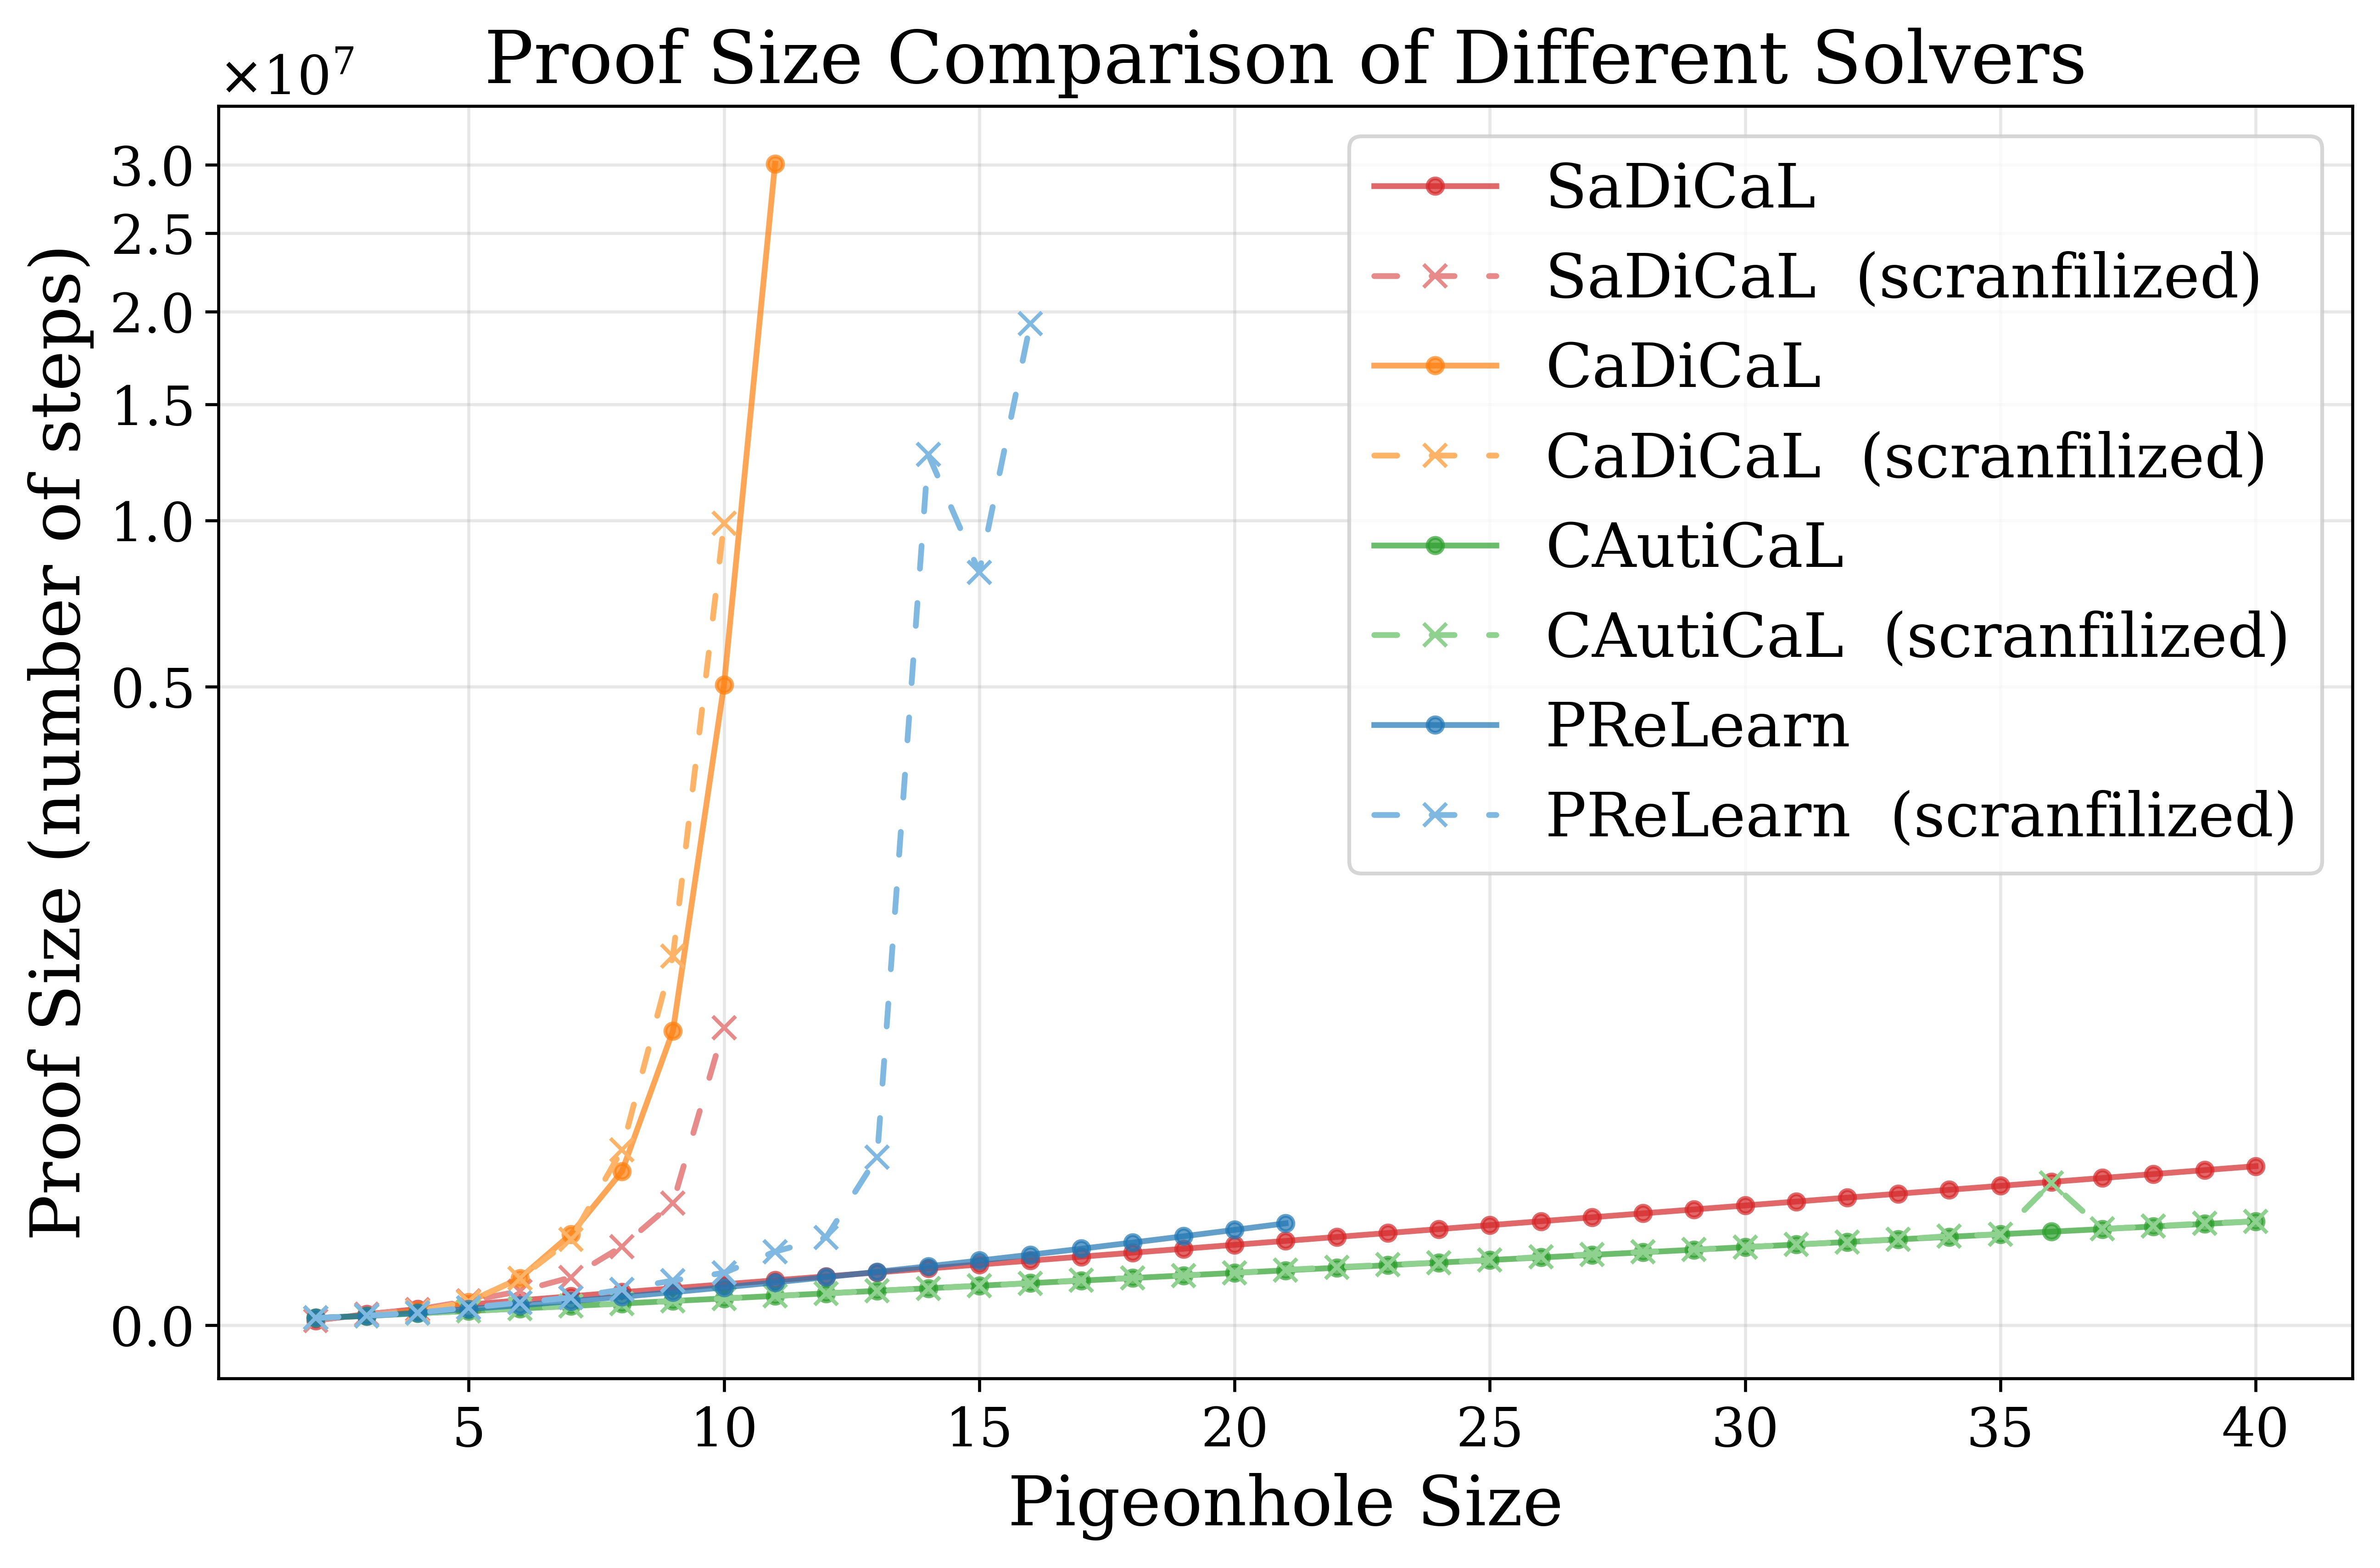
\includegraphics[width=\textwidth]{figs/pigeonhole_proof_size_comparison.jpg}
        % \caption{Proof Size for Pigeonhole Principle Formulas}
        \label{fig:pigeonhole-proof-size-comparison}
    \end{subfigure}
    \caption{Comparison of \tool, \cadical, \sadical, and \prelearn on pigeonhole principle benchmarks up to size $40$. The y-axis is on a cube root scale. The performance of a solver on the original benchmark is shown with a solid line. The median of 5 scranfilized queries is shown with a dashed line. If a solver times out on a query in 5000s, it is not shown.}
    \label{fig:pigeonhole-results}
\end{figure*}


Approaches based on SDCL, such as \sadical, are successful for learning $O(n^3)$ proofs for the pigeonhole
principle, but are very sensitive to the encoding of the formula. We compare the solvers on
pigeonhole principle from \ph{2} to \ph{40} and plot these results in \autoref{fig:pigeonhole-results}. As the expected best-behavior is cubic, we use a cube root scale for the y-axis.

As expected, \cadical grows exponentially, while \sadical and \tool scale cubicly in both runtime and proof size. Significantly, \tool is able to learn $3.59$-$3.64$x shorter proofs compared to \sadical. 
% on formulas larger than \ph{10}
This is because \sadical deletes clauses more frequently, as to not exclude other clauses from being learned. Frequent deletion is not necessary in \tool because of its clause shrinking technique.
\prelearn scales cubicly on small formulas, but for \ph{22} and larger, will not learn enough useful \pr clauses in the preprocessing step and times out.

% As we discuss in
% \autoref{app:pigeonhole}, \tool learns proofs of size $\approx \frac13 n^3$,
% which is expected to be shorter than known \pr proofs for the pigeonhole principle.

Additionally, we evaluate all solvers on scranfilized variations of the
pigeonhole principle. Scranfilization is a technique for generating an
equivalently satisfiable formula~\cite{scranfilize}. We use the tool
\texttt{scranfilize} with permuting variables, permuting clauses, and flipping literals (with probability $0.5$) all turned on~\cite{scranfilize}. We run each solver on 5 scranfilized variations for
each benchmark and take the median runtime and proof size. This is shown in \autoref{fig:pigeonhole-results} with dashed lines.

\sadical and \prelearn exhibit an exponential trend for runtime and proof size on the scranfilized benchmarks. \sadical will spend all its time in the main SDCL loop not learning enough useful clauses. \prelearn will learn some useful \pr clauses in preprocessing, but not enough to sufficiently shrink the search space for formulas larger than \ph{16}.

On the other hand, \tool almost matches its non-scranfilized performance, demonstrating that it learns useful \pr clauses regardless of the encoding.

% In conclusion, \tool is able to match \sadical's runtime for the pigeonhole principle while shorter proofs by a constant factor. Additionally, \tool is insensitive to permuting variables, permuting clauses, and flipping literals as it relies on conditional autarkies, a global property of the formula.



\subsection{SATCOMP results}~\label{subsec:eval-satcomp}

% \begin{figure*}[!t]
%     \centering
%     \begin{subfigure}[t]{0.4\textwidth}
%         \centering
%         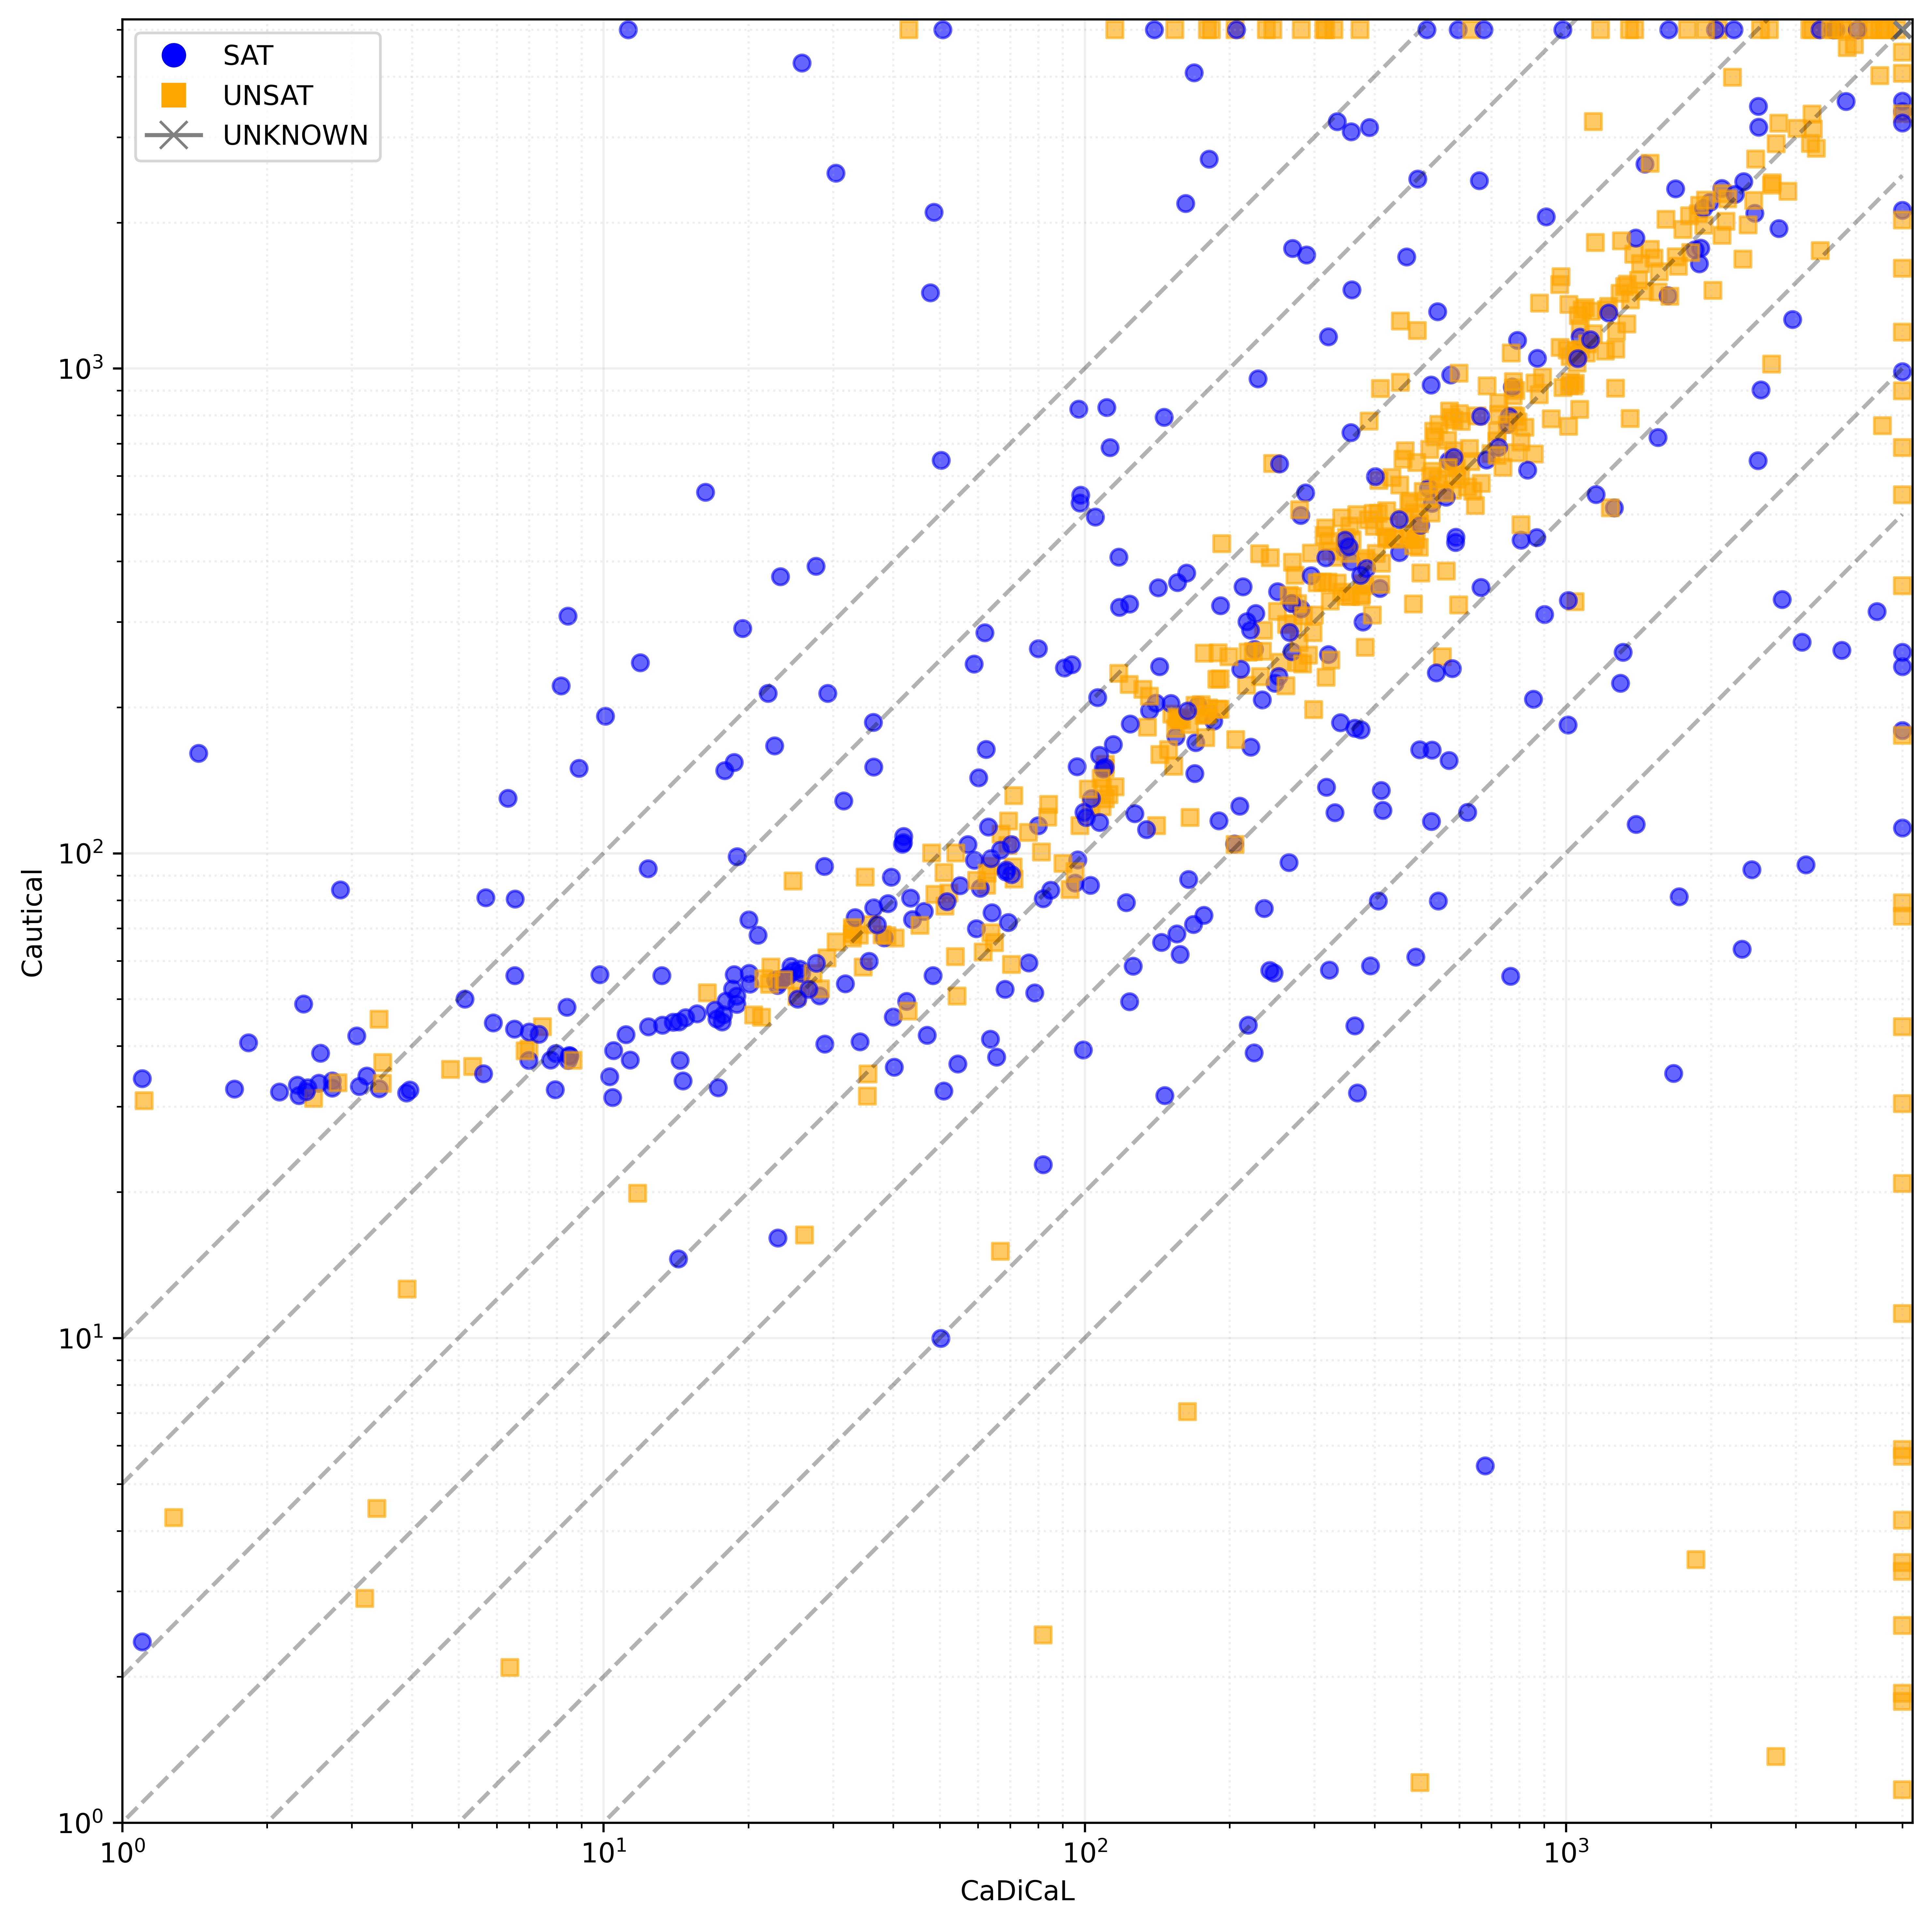
\includegraphics[width=\textwidth]{figs/cautical_vs_cadical_log.png}
%         \caption{Comparison with \cadical}
%         \label{fig:cautical-vs-cadical}
%     \end{subfigure}
%     \hspace{0.06\textwidth}
%     \begin{subfigure}[t]{0.4\textwidth}
%         \centering
%         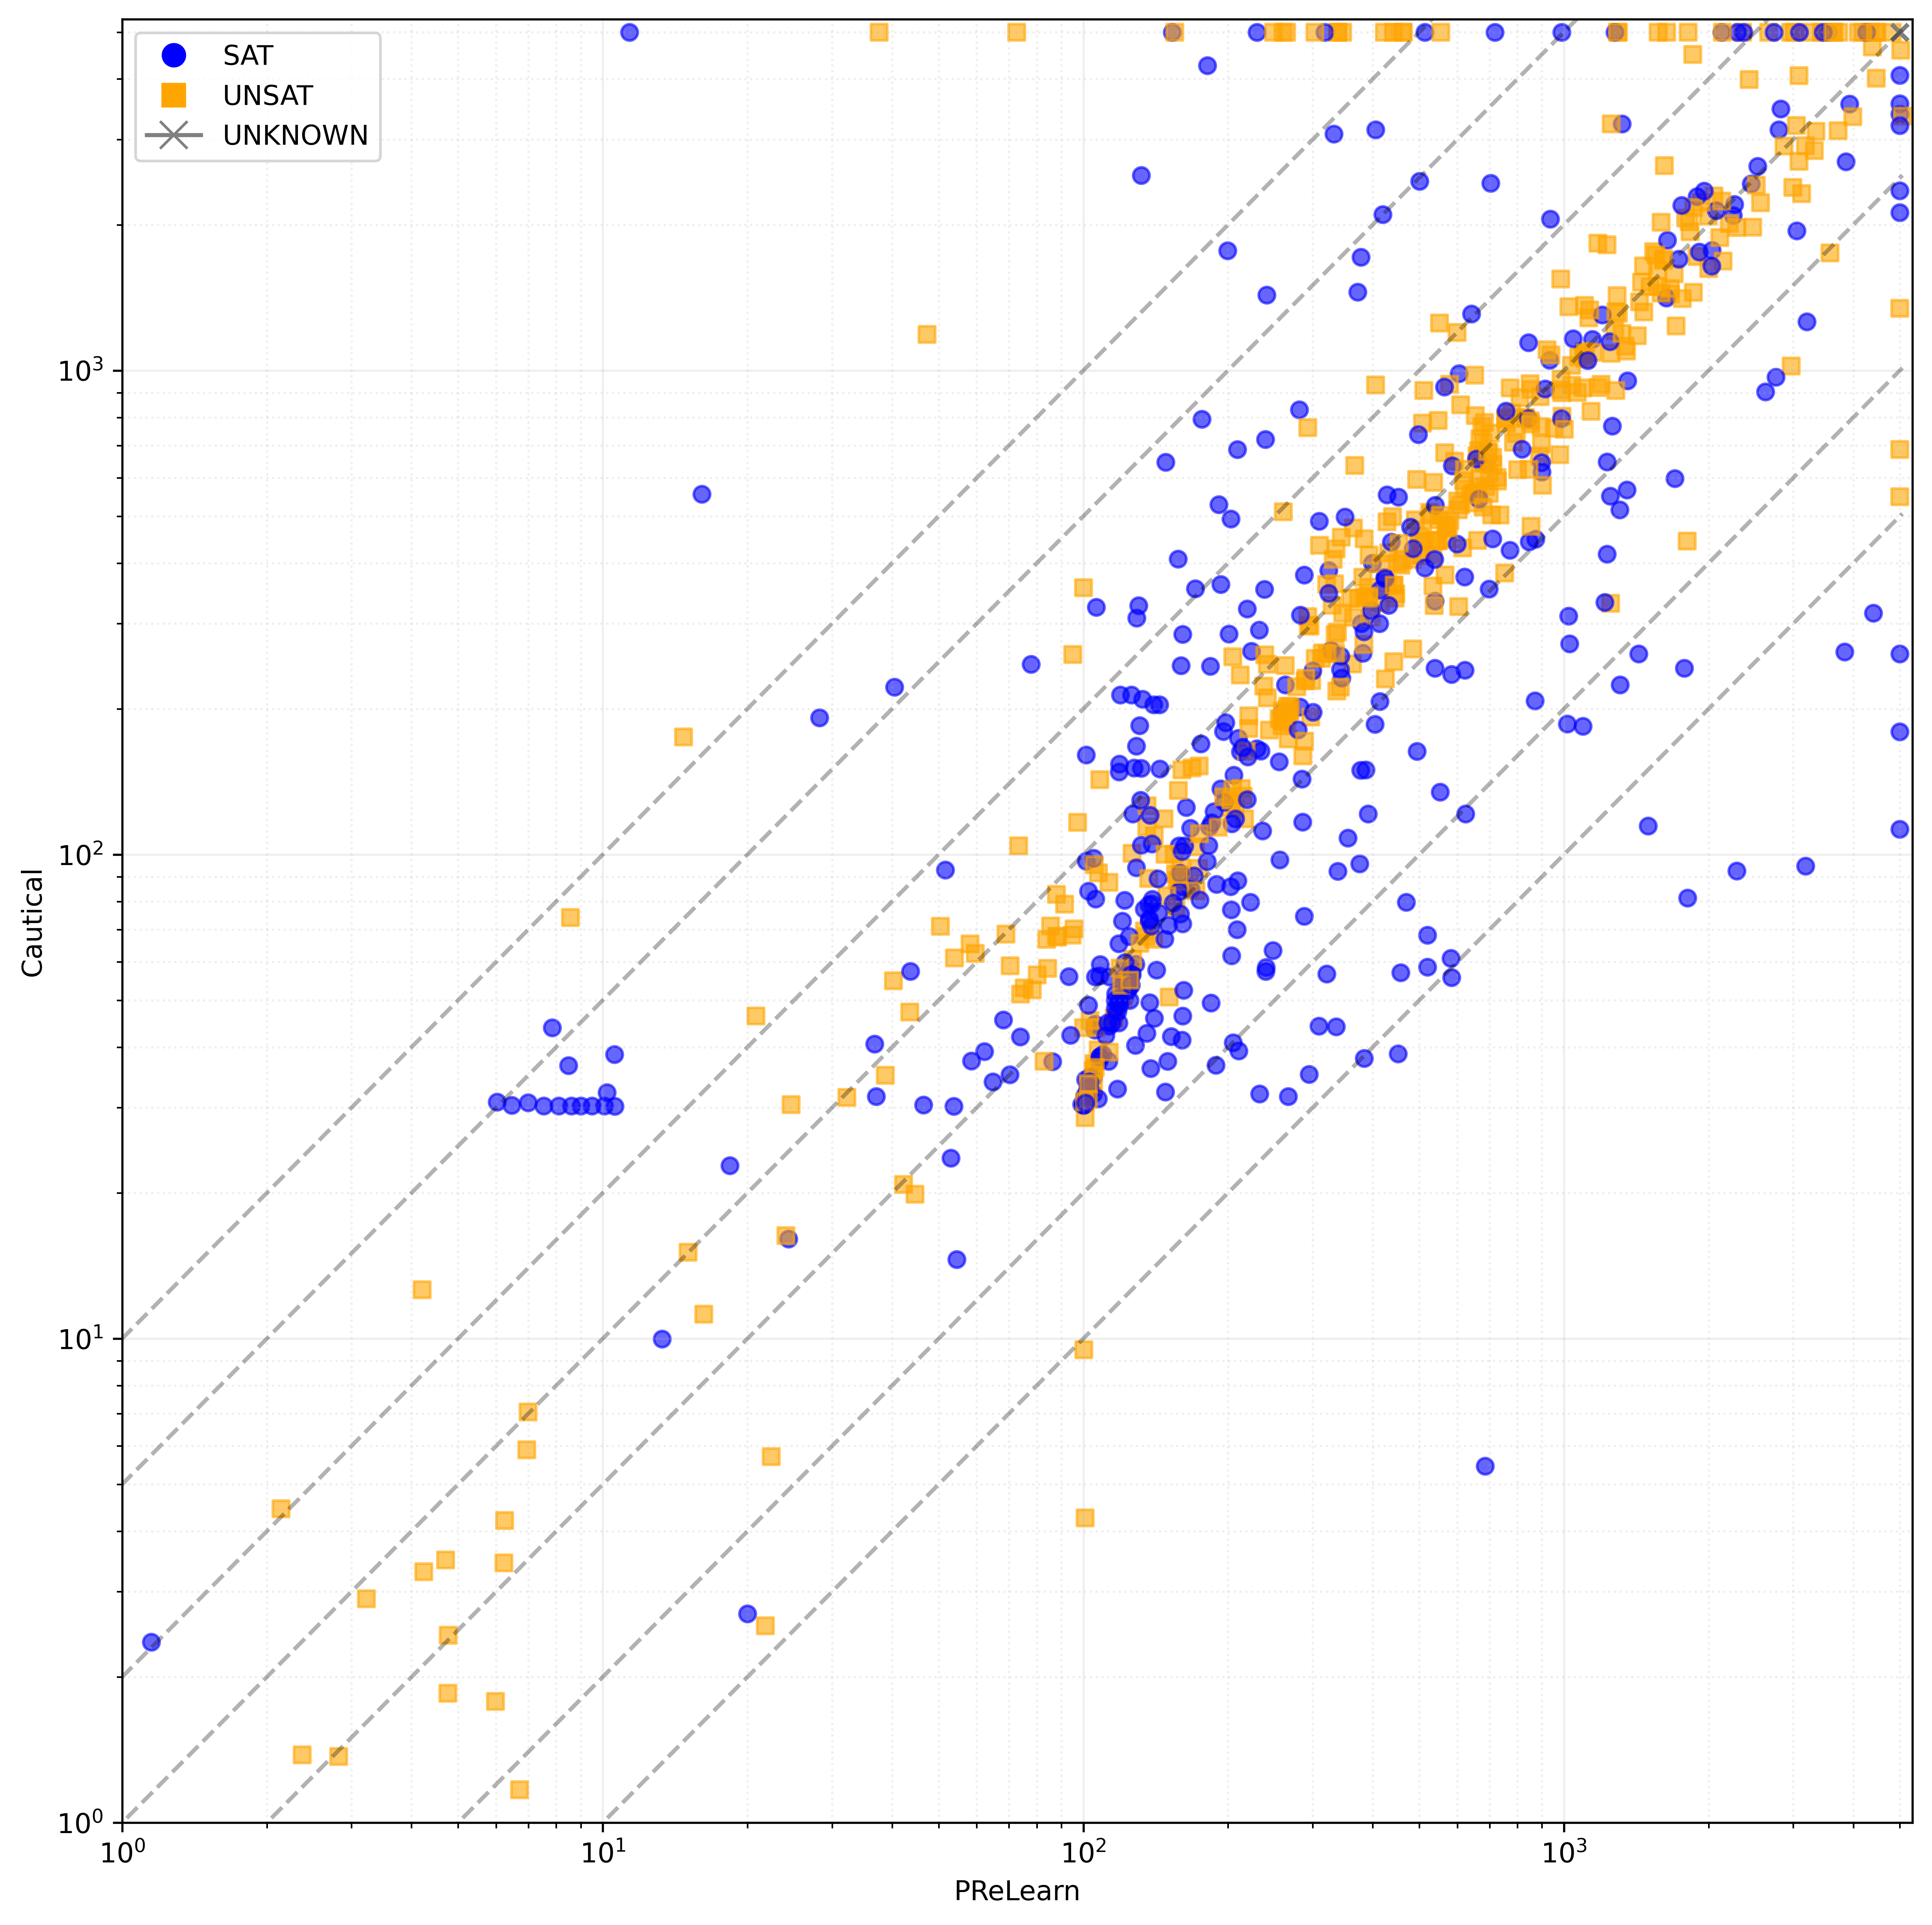
\includegraphics[width=\textwidth]{figs/cautical_vs_prelearn_log.png}
%         \caption{Comparison with \prelearn}
%         \label{fig:cautical-vs-prelearn}
%     \end{subfigure}
%     \caption{Performance comparison of \tool with other solvers}
%     \label{fig:solver-comparison}
% \end{figure*}


% \begin{figure*}[!t]
%     \centering
%     \begin{subfigure}[t]{0.4\textwidth}
%         \centering
%         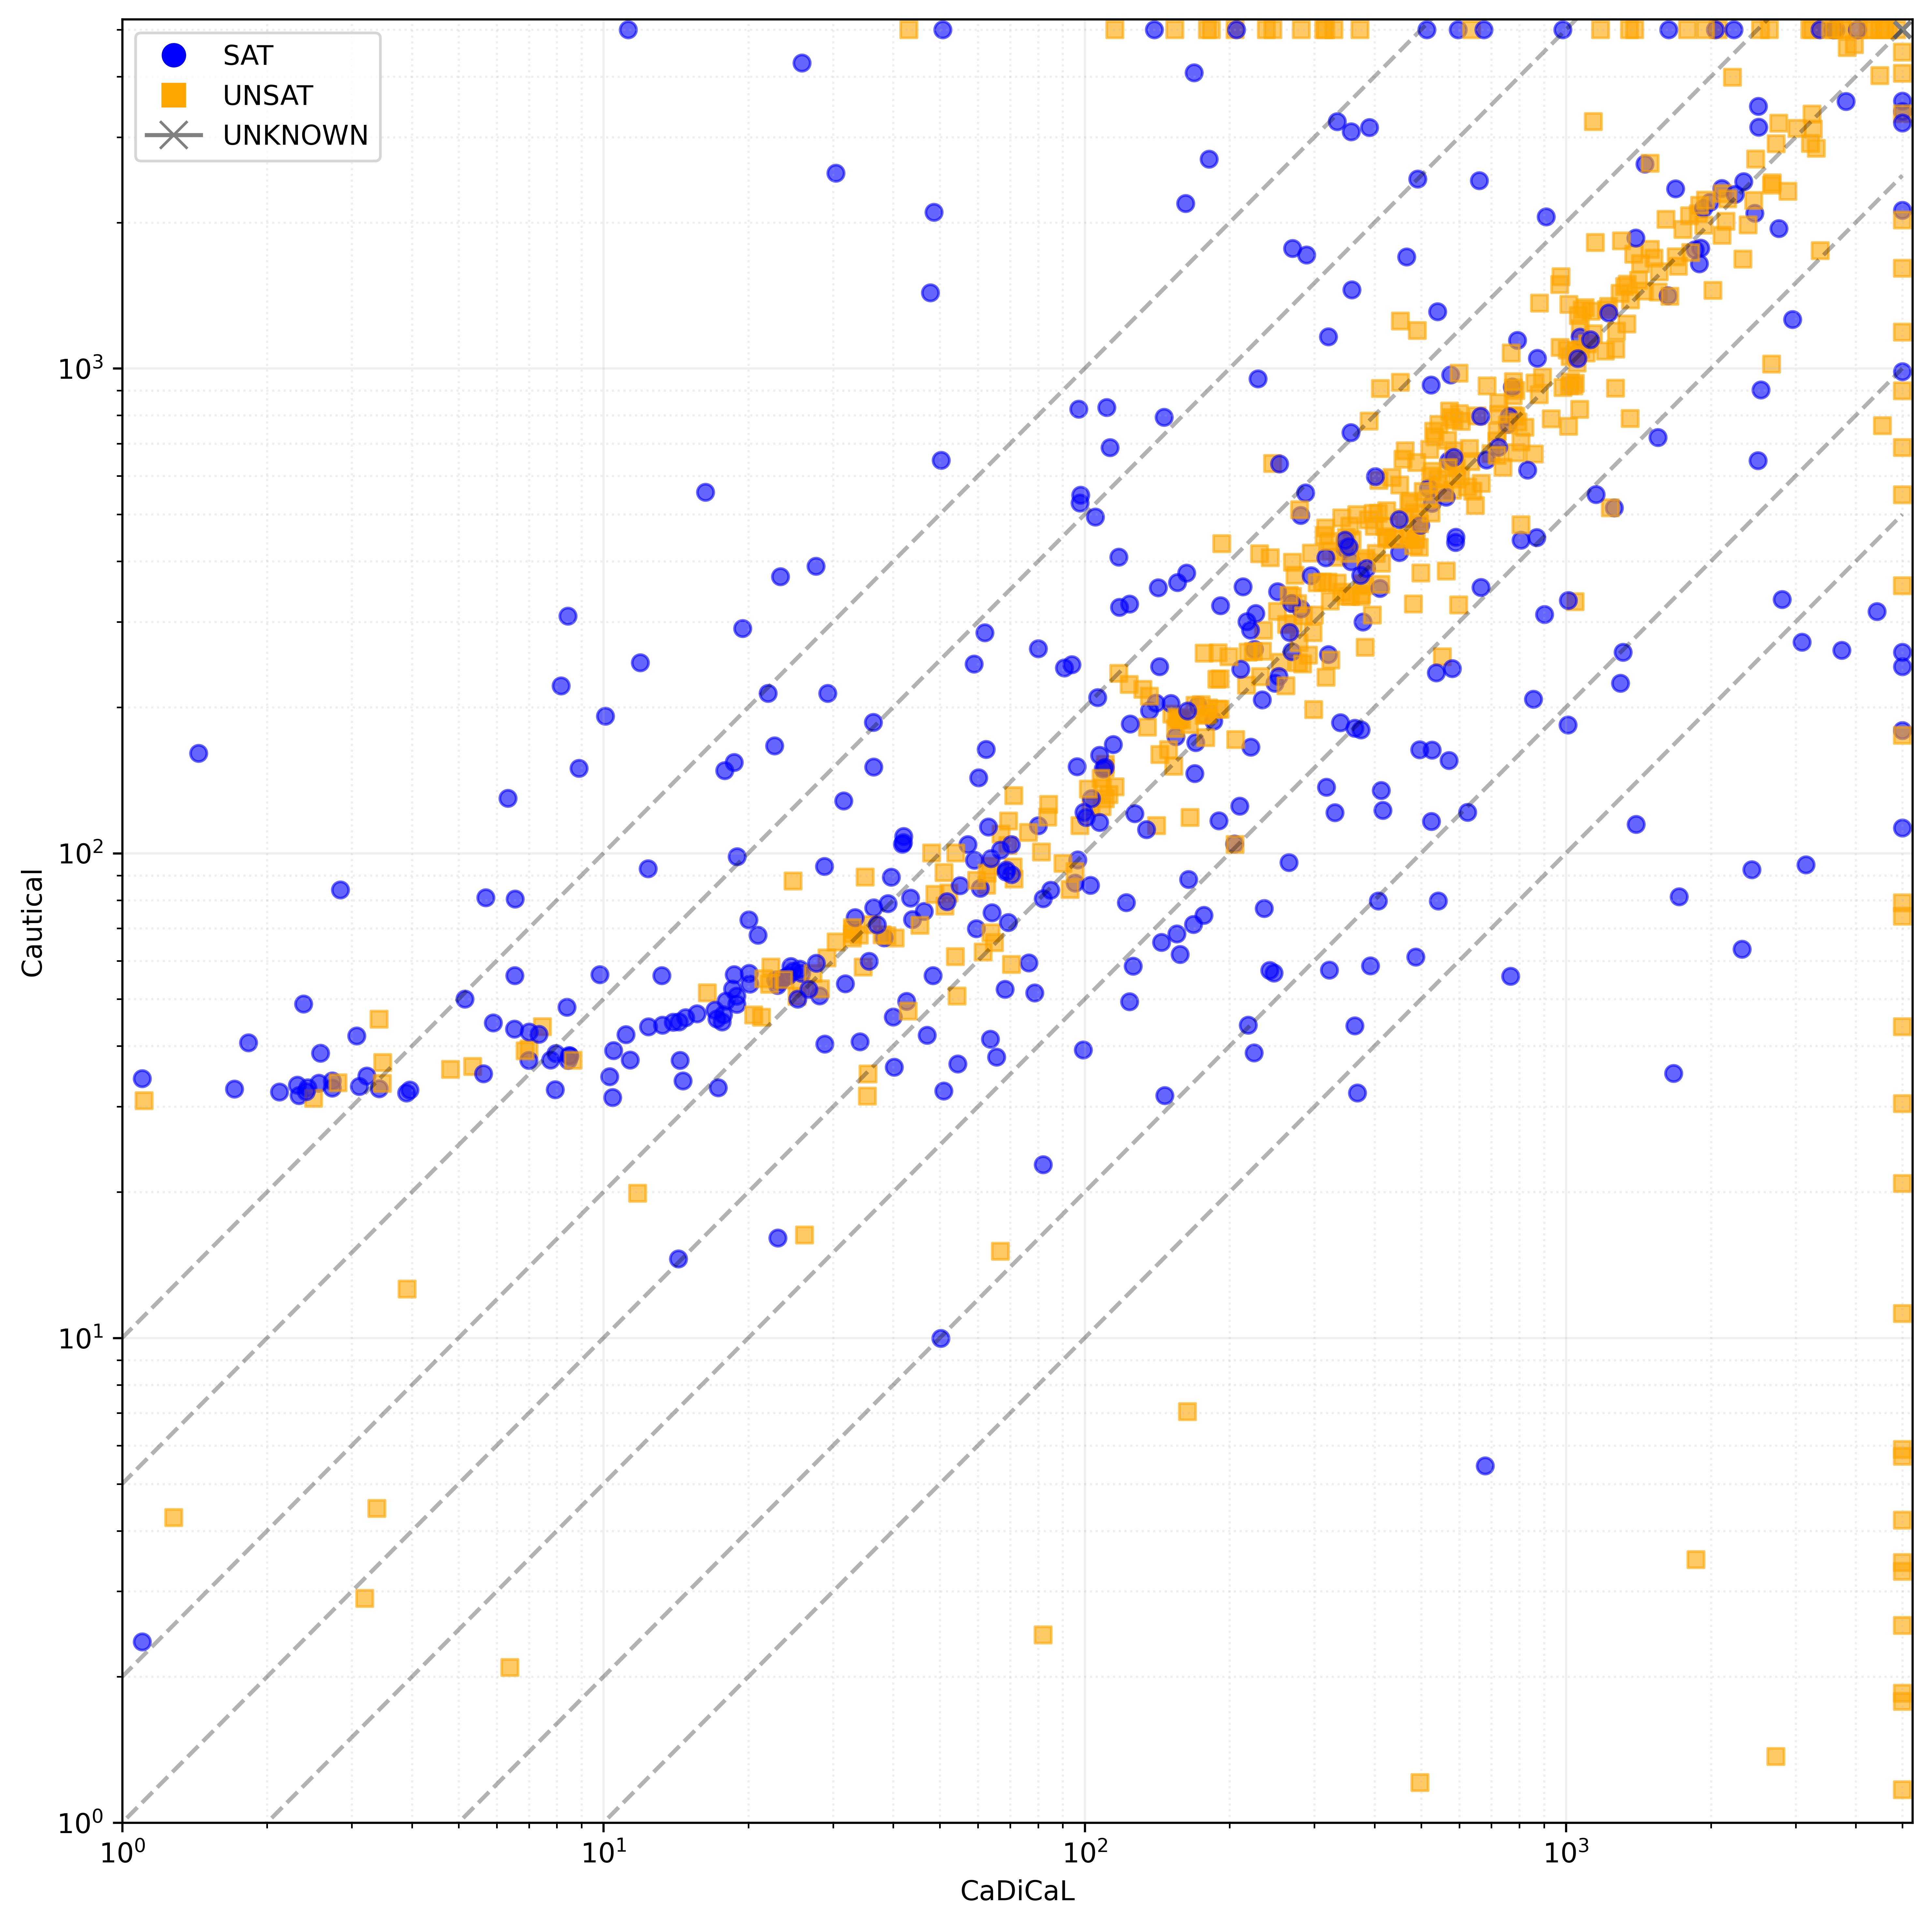
\includegraphics[width=\textwidth]{figs/cautical_vs_cadical_log.png}
%         \caption{Comparison with \cadical}
%         \label{fig:cautical-vs-cadical}
%     \end{subfigure}
%     \hspace{0.06\textwidth}
%     \begin{subfigure}[t]{0.4\textwidth}
%         \centering
%         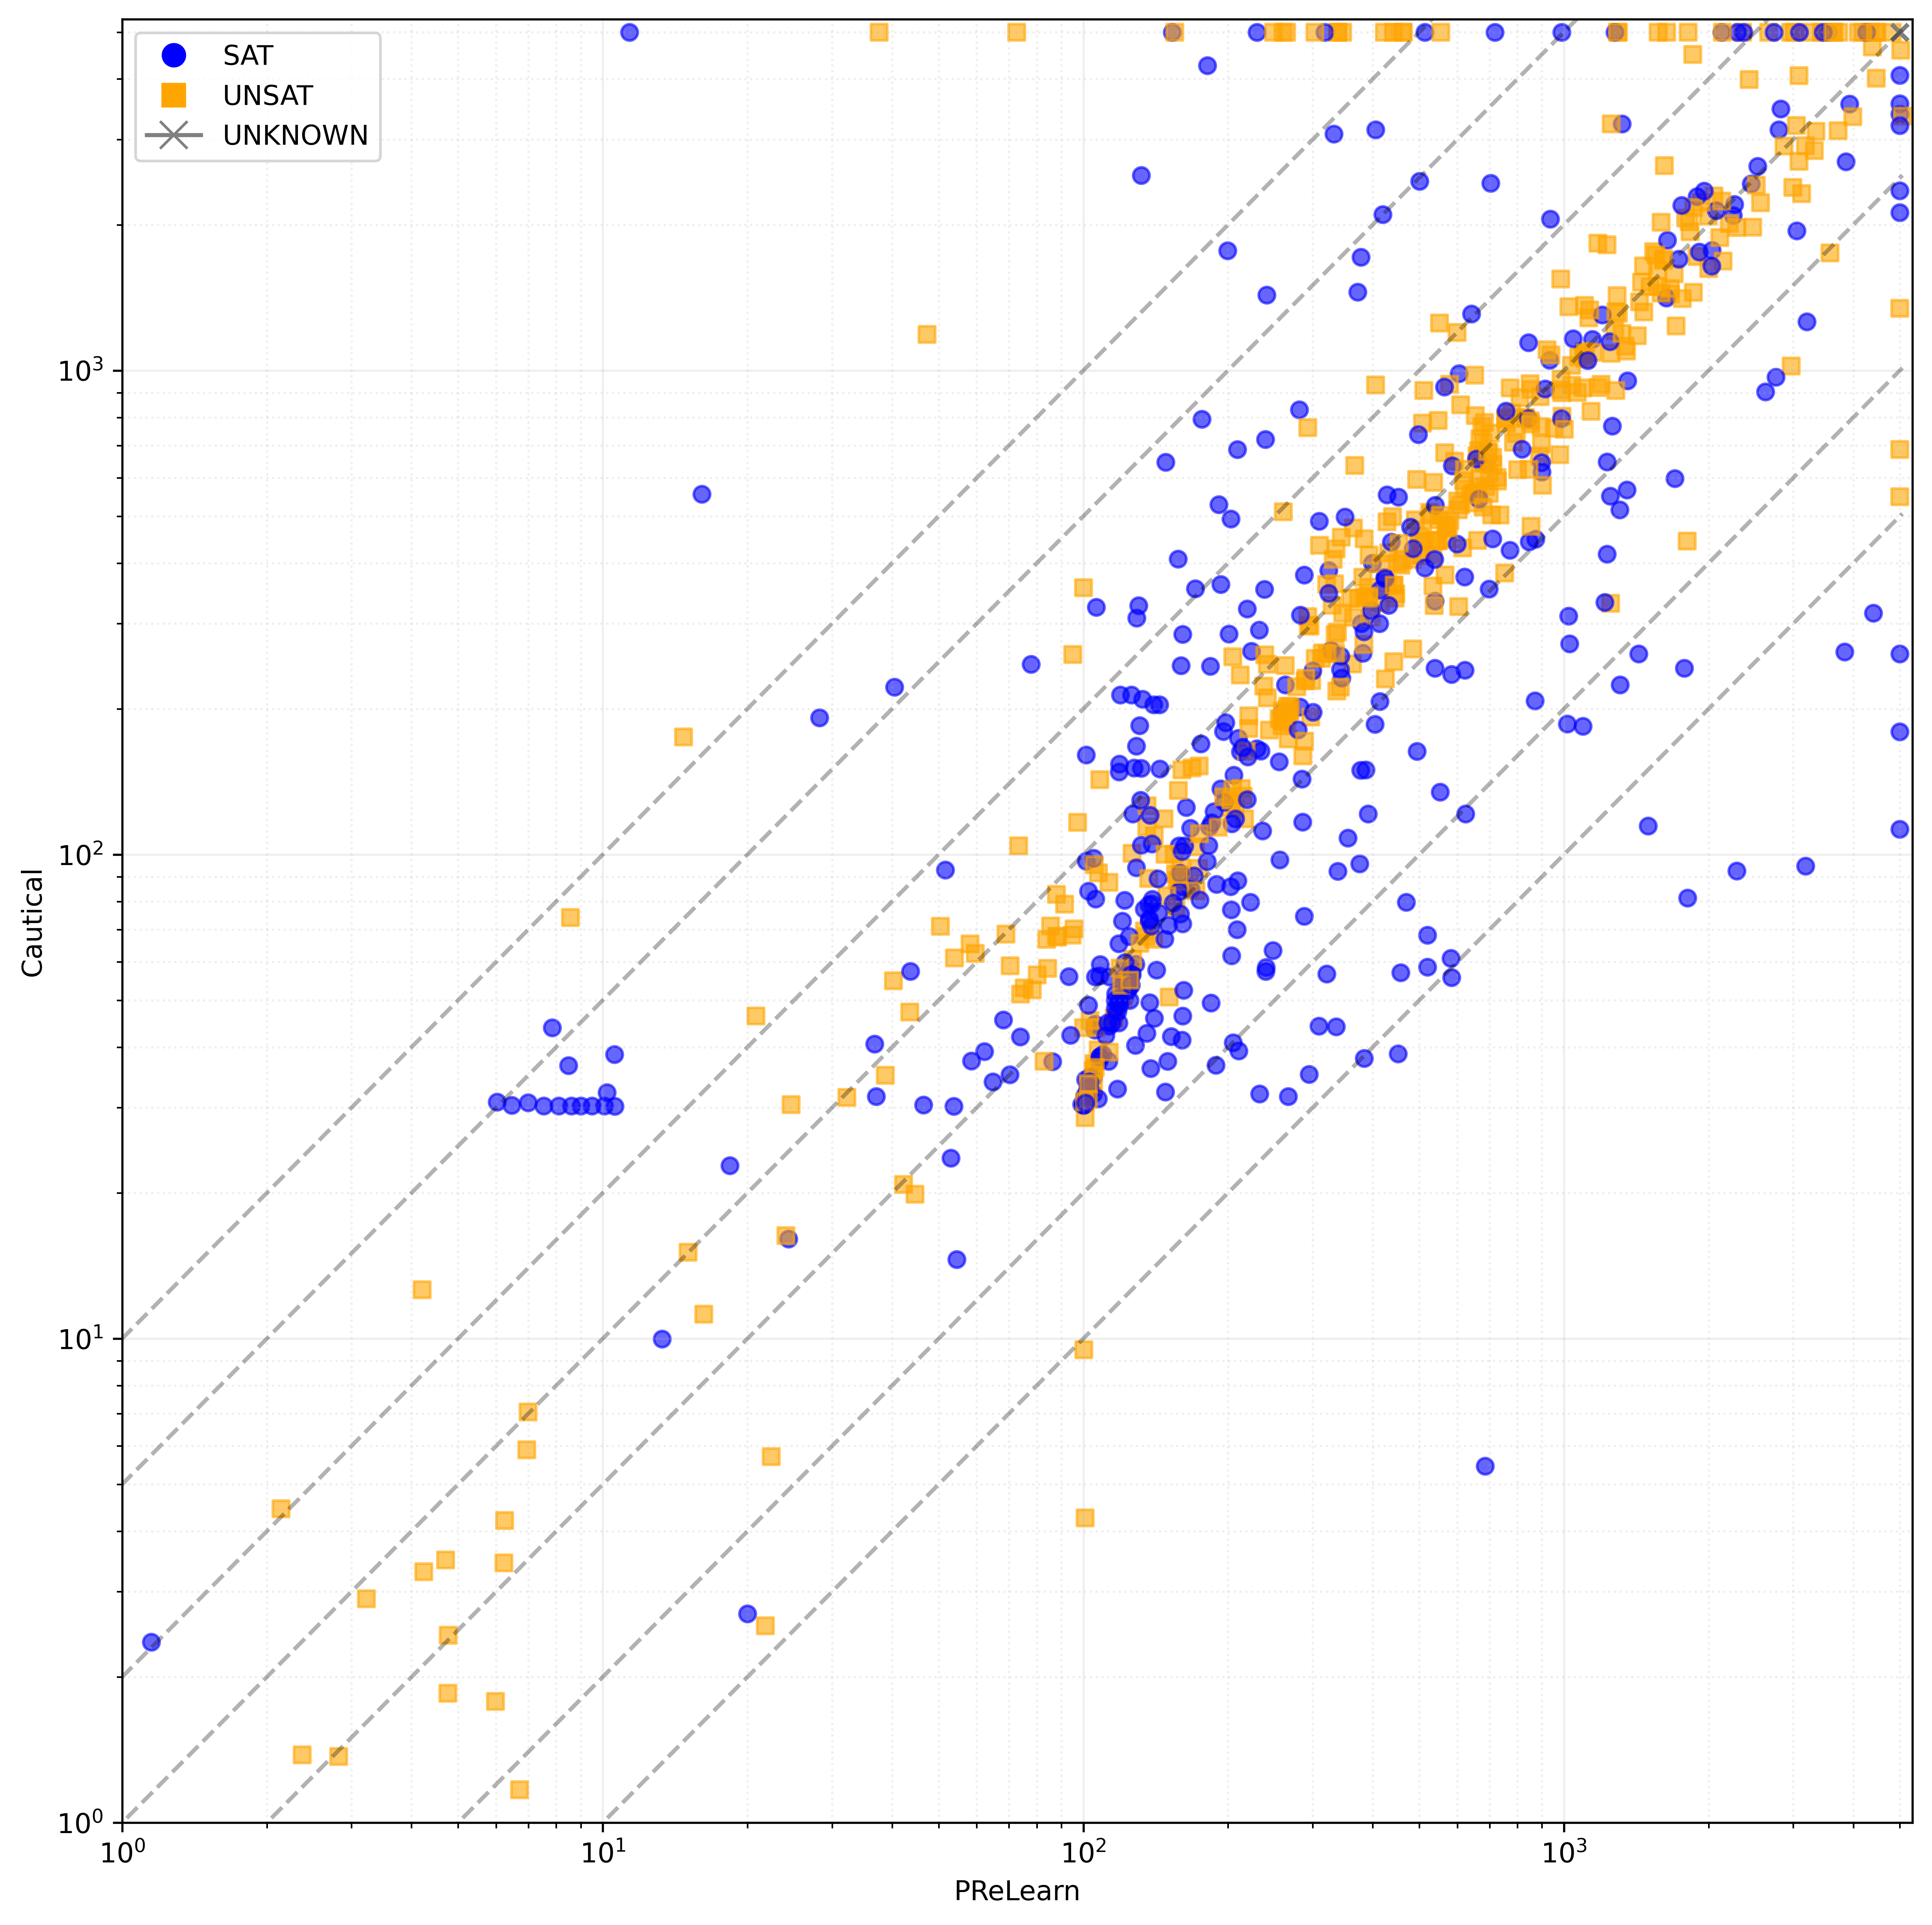
\includegraphics[width=\textwidth]{figs/cautical_vs_prelearn_log.png}
%         \caption{Comparison with \prelearn}
%         \label{fig:cautical-vs-prelearn}
%     \end{subfigure}
%     \caption{Performance comparison of \tool with other solvers}
%     \label{fig:solver-comparison}
% \end{figure*}


\begin{figure*}[!t]
    \centering
    \begin{subfigure}[t]{0.3\textwidth}
        \centering
        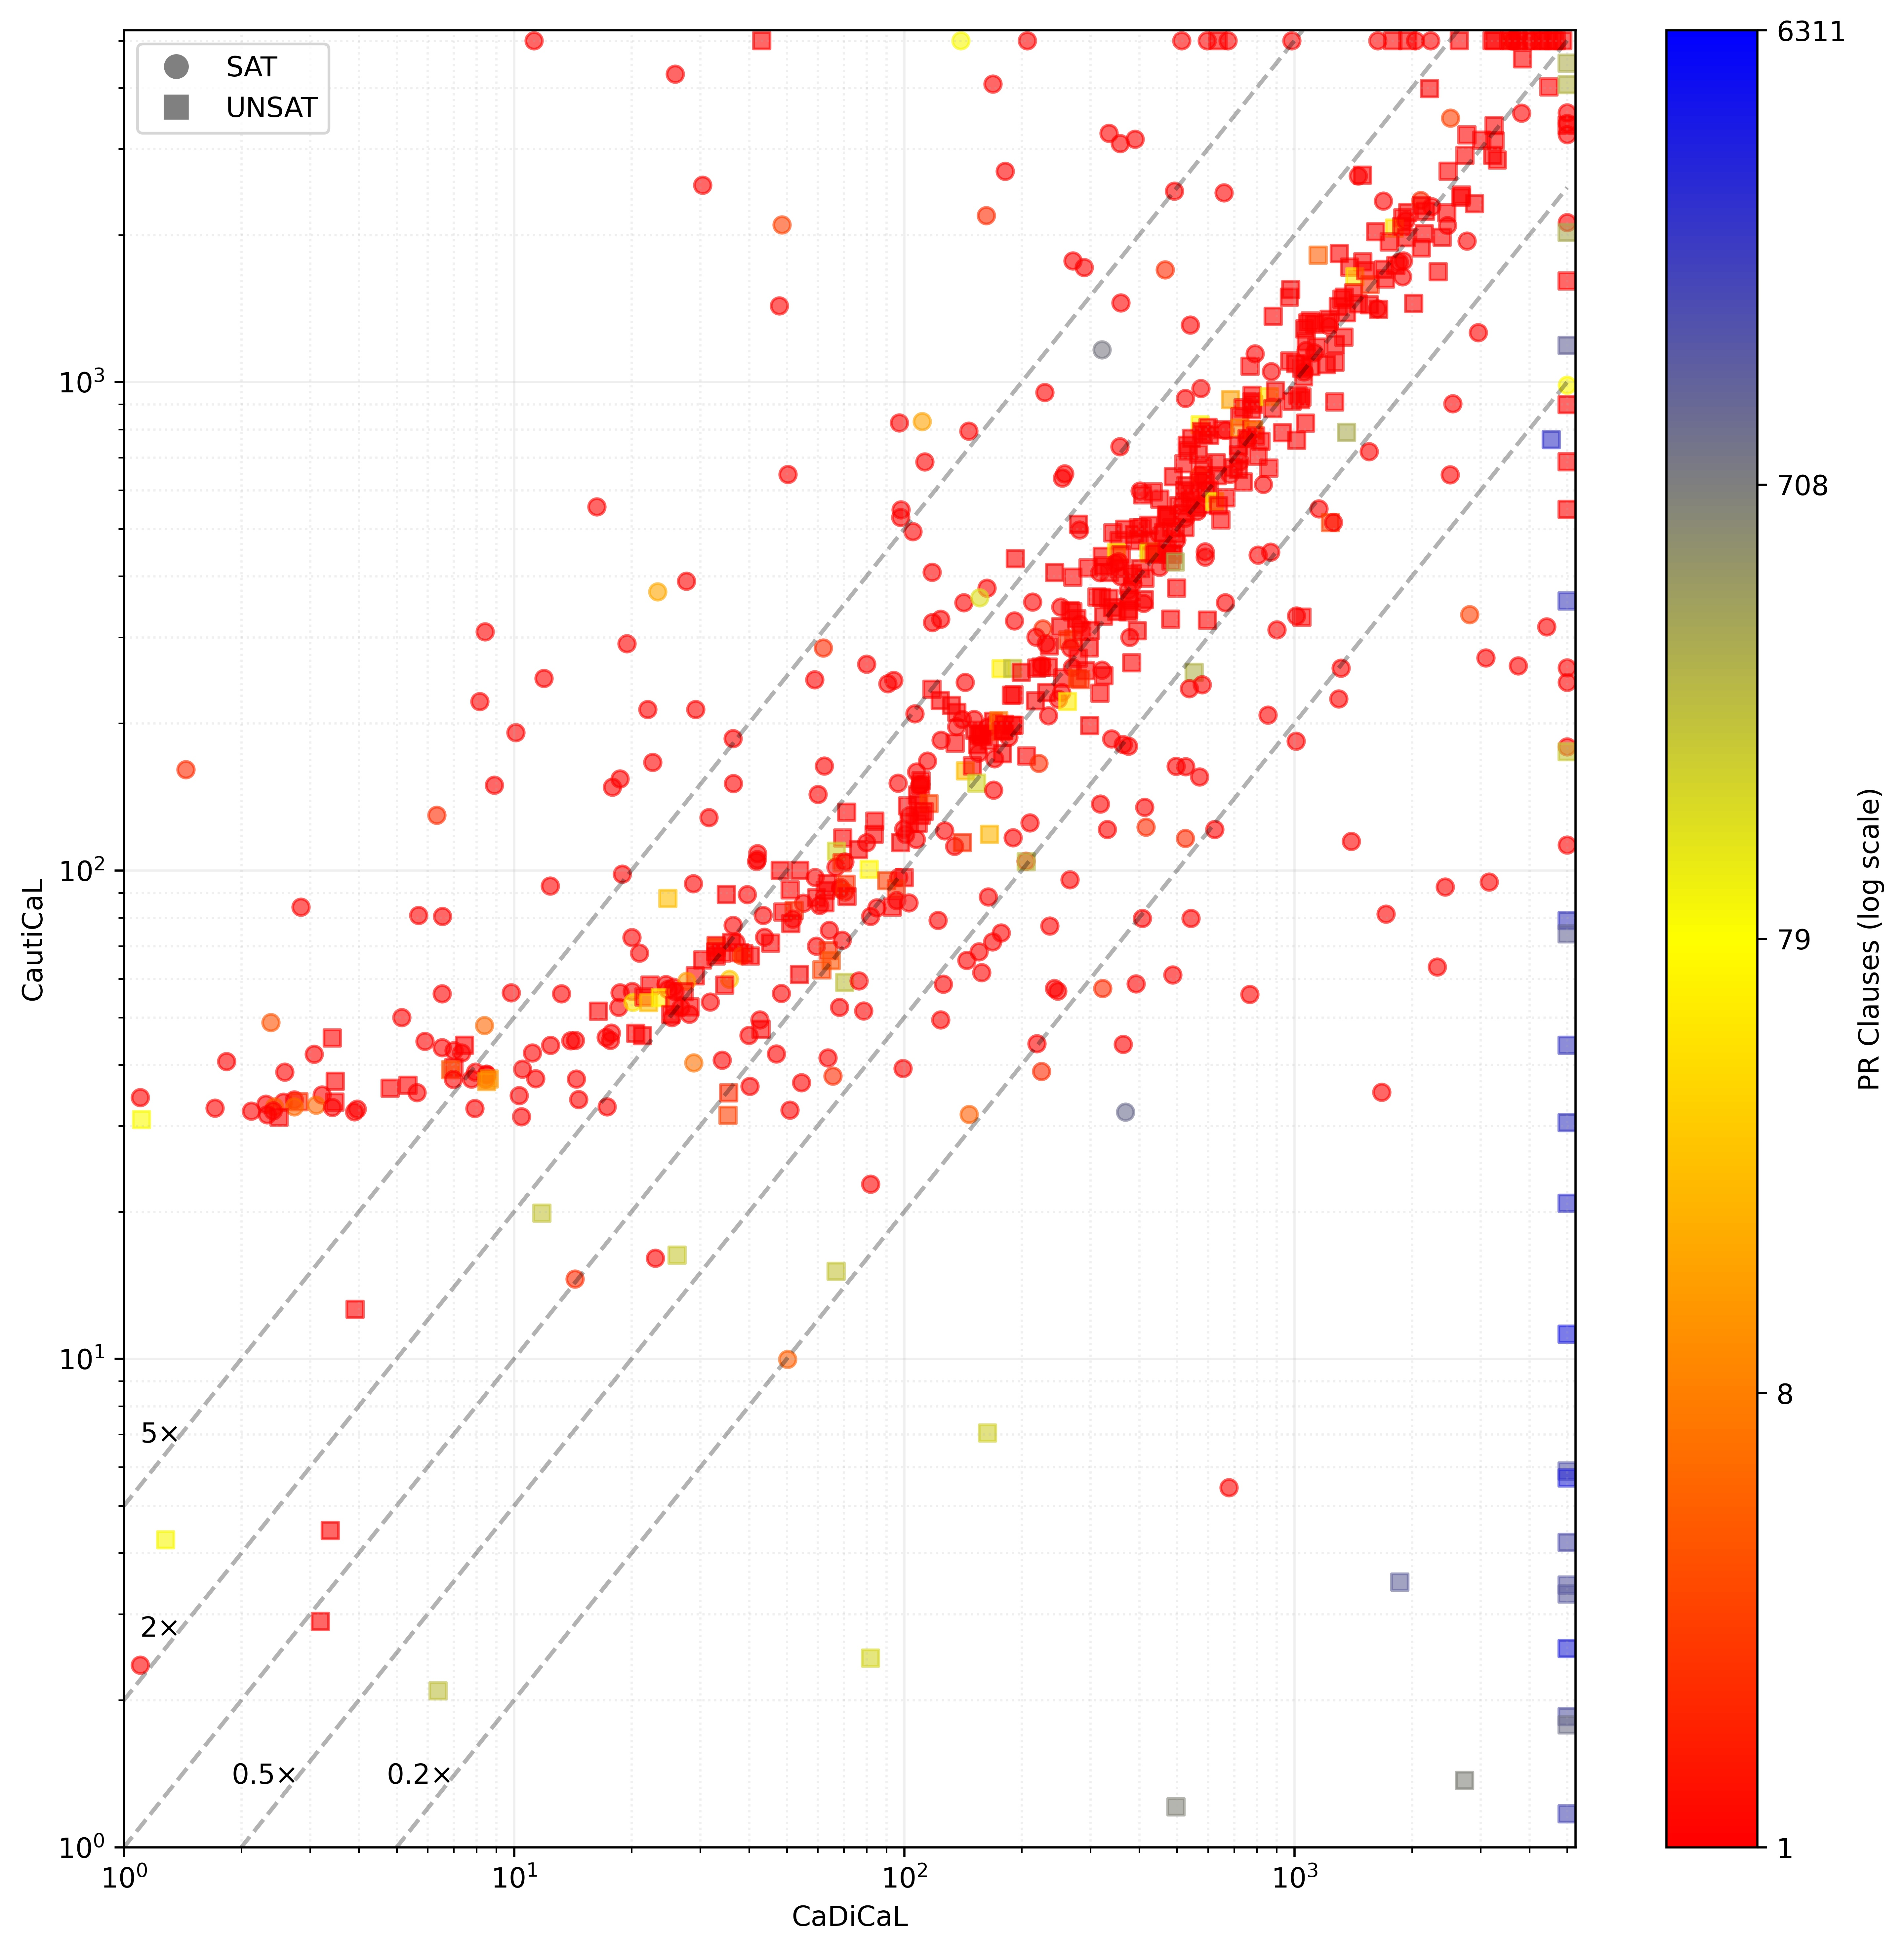
\includegraphics[width=\textwidth]{figs/cadical_vs_cautical.jpg}
        \caption{Comparison with \cadical}
        \label{fig:cautical-vs-cadical}
    \end{subfigure}
    % \hspace{0.06\textwidth}
    \begin{subfigure}[t]{0.3\textwidth}
        \centering
        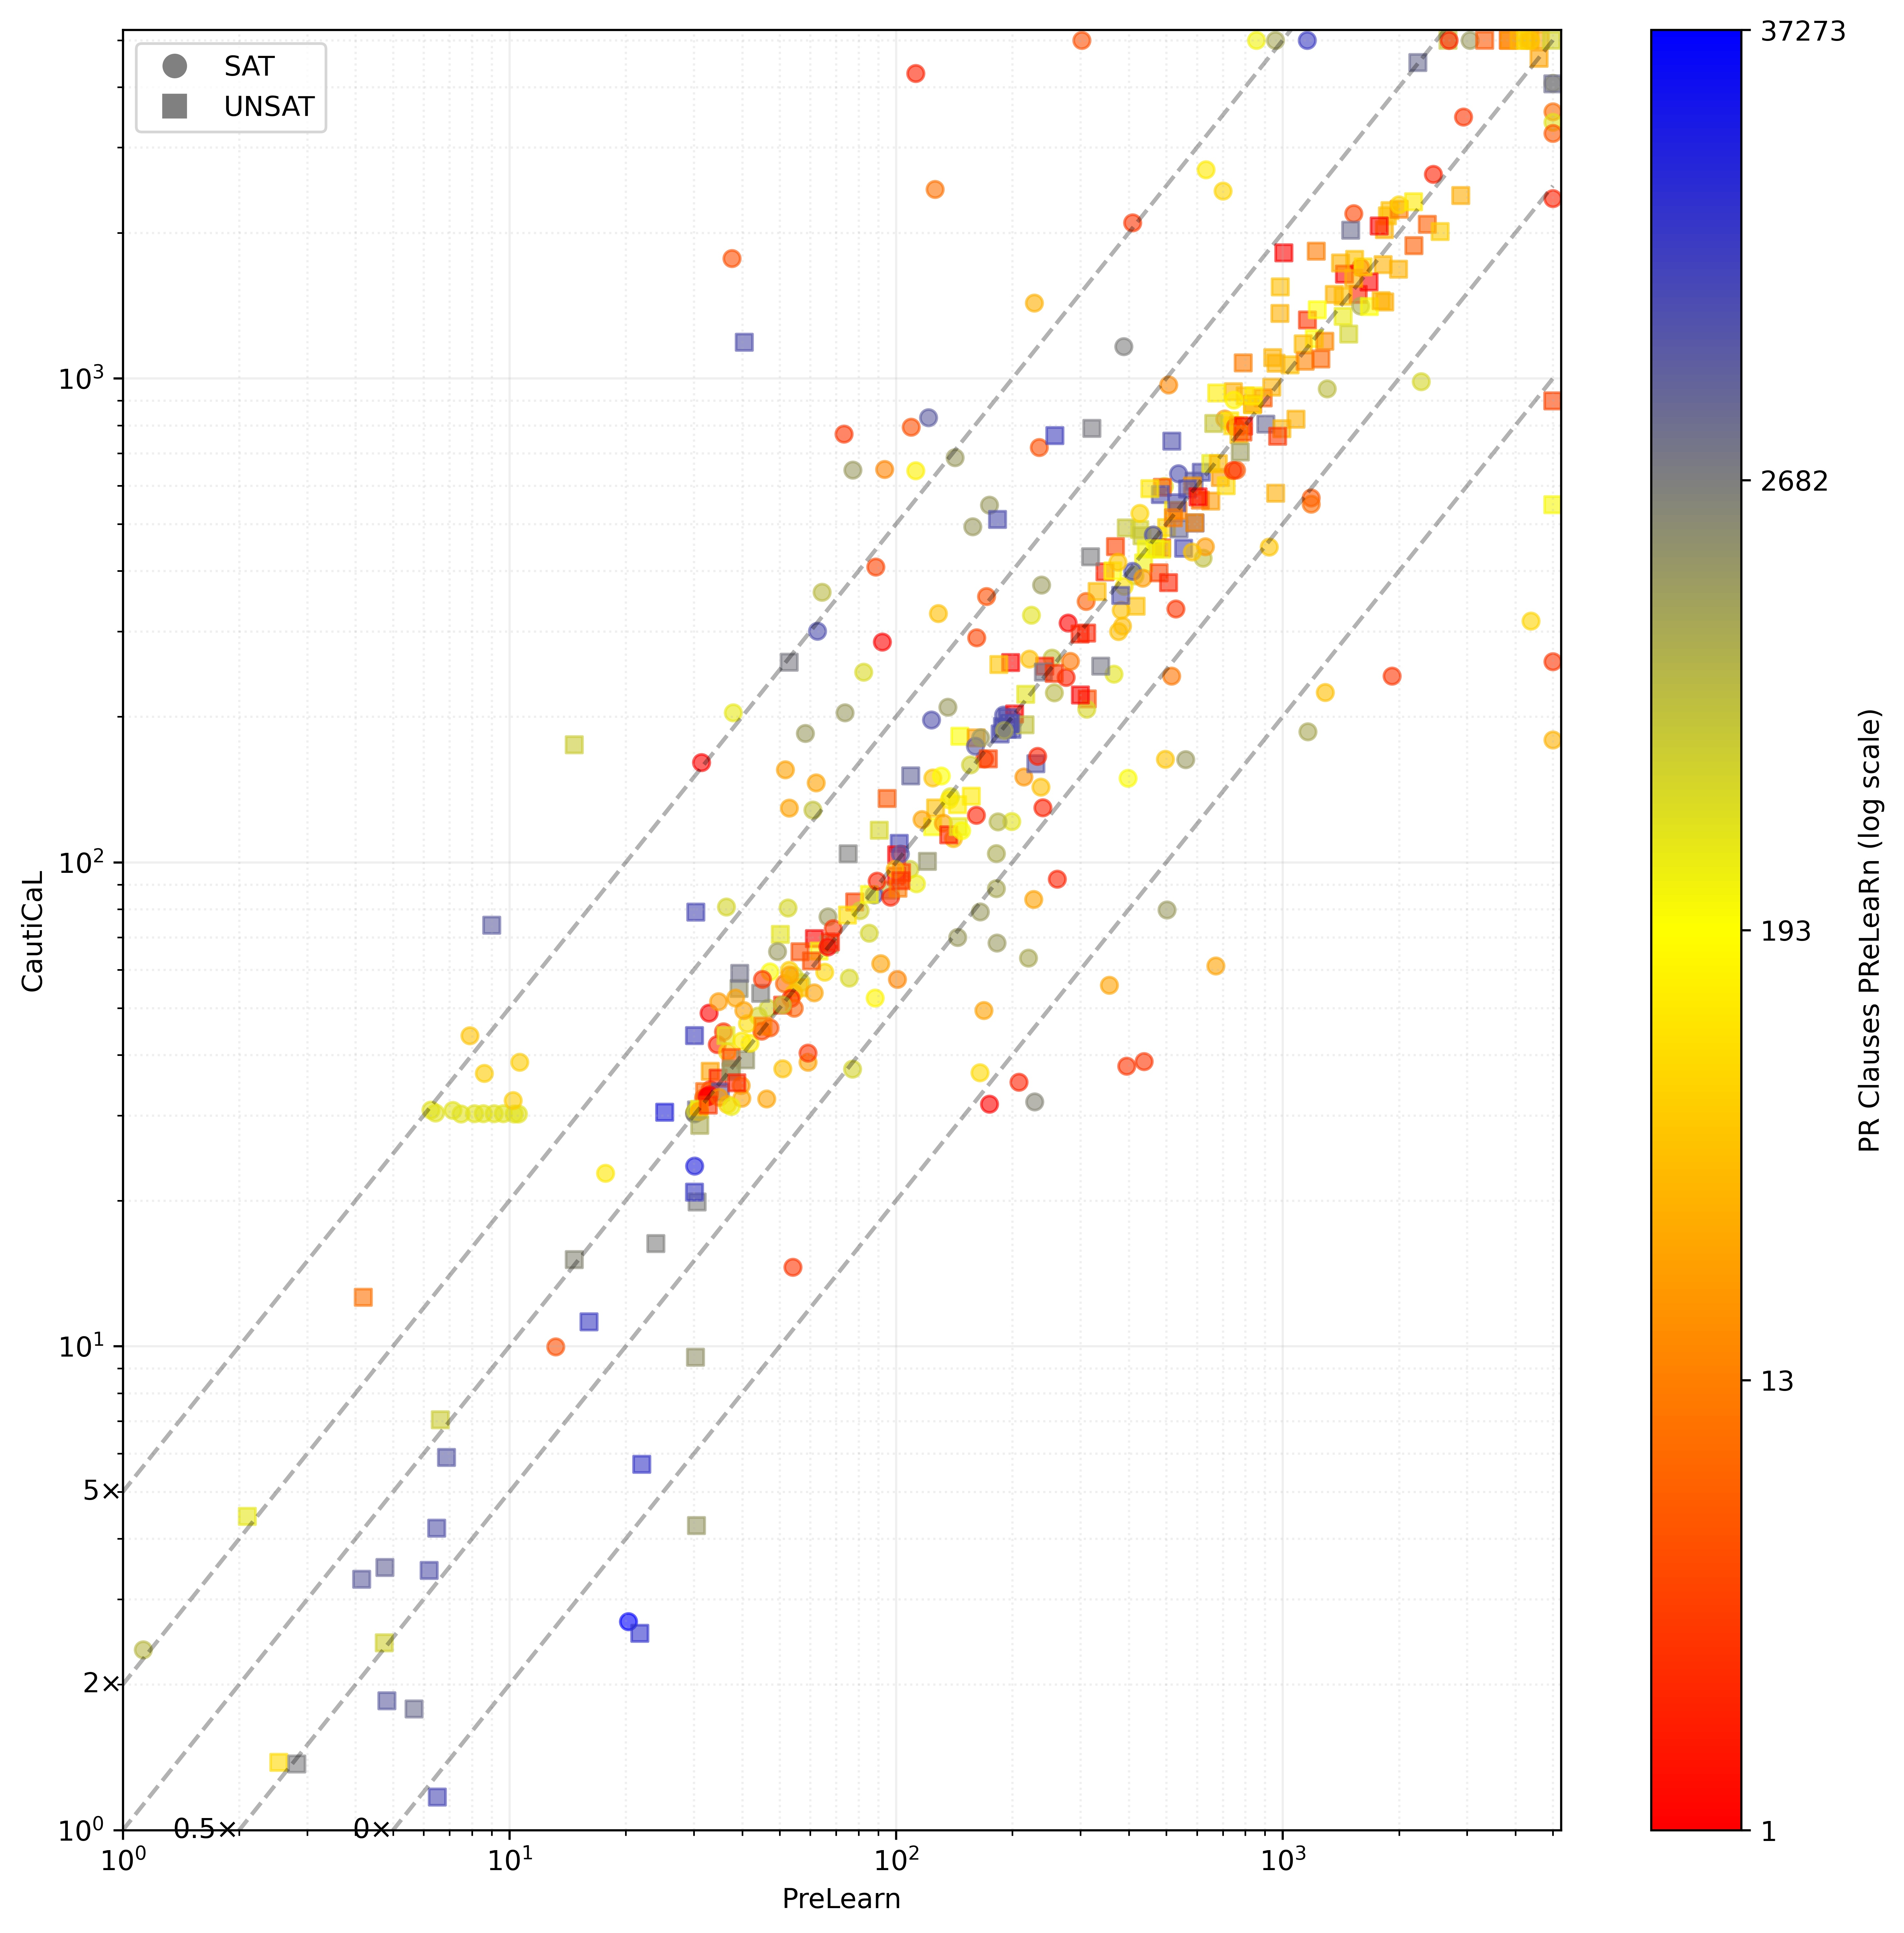
\includegraphics[width=\textwidth]{figs/prelearn_vs_cautical.jpg}
        \caption{Comparison with \prelearn}
        \label{fig:cautical-vs-prelearn}
    \end{subfigure}
    \begin{subfigure}[t]{0.3\textwidth}
        \centering
        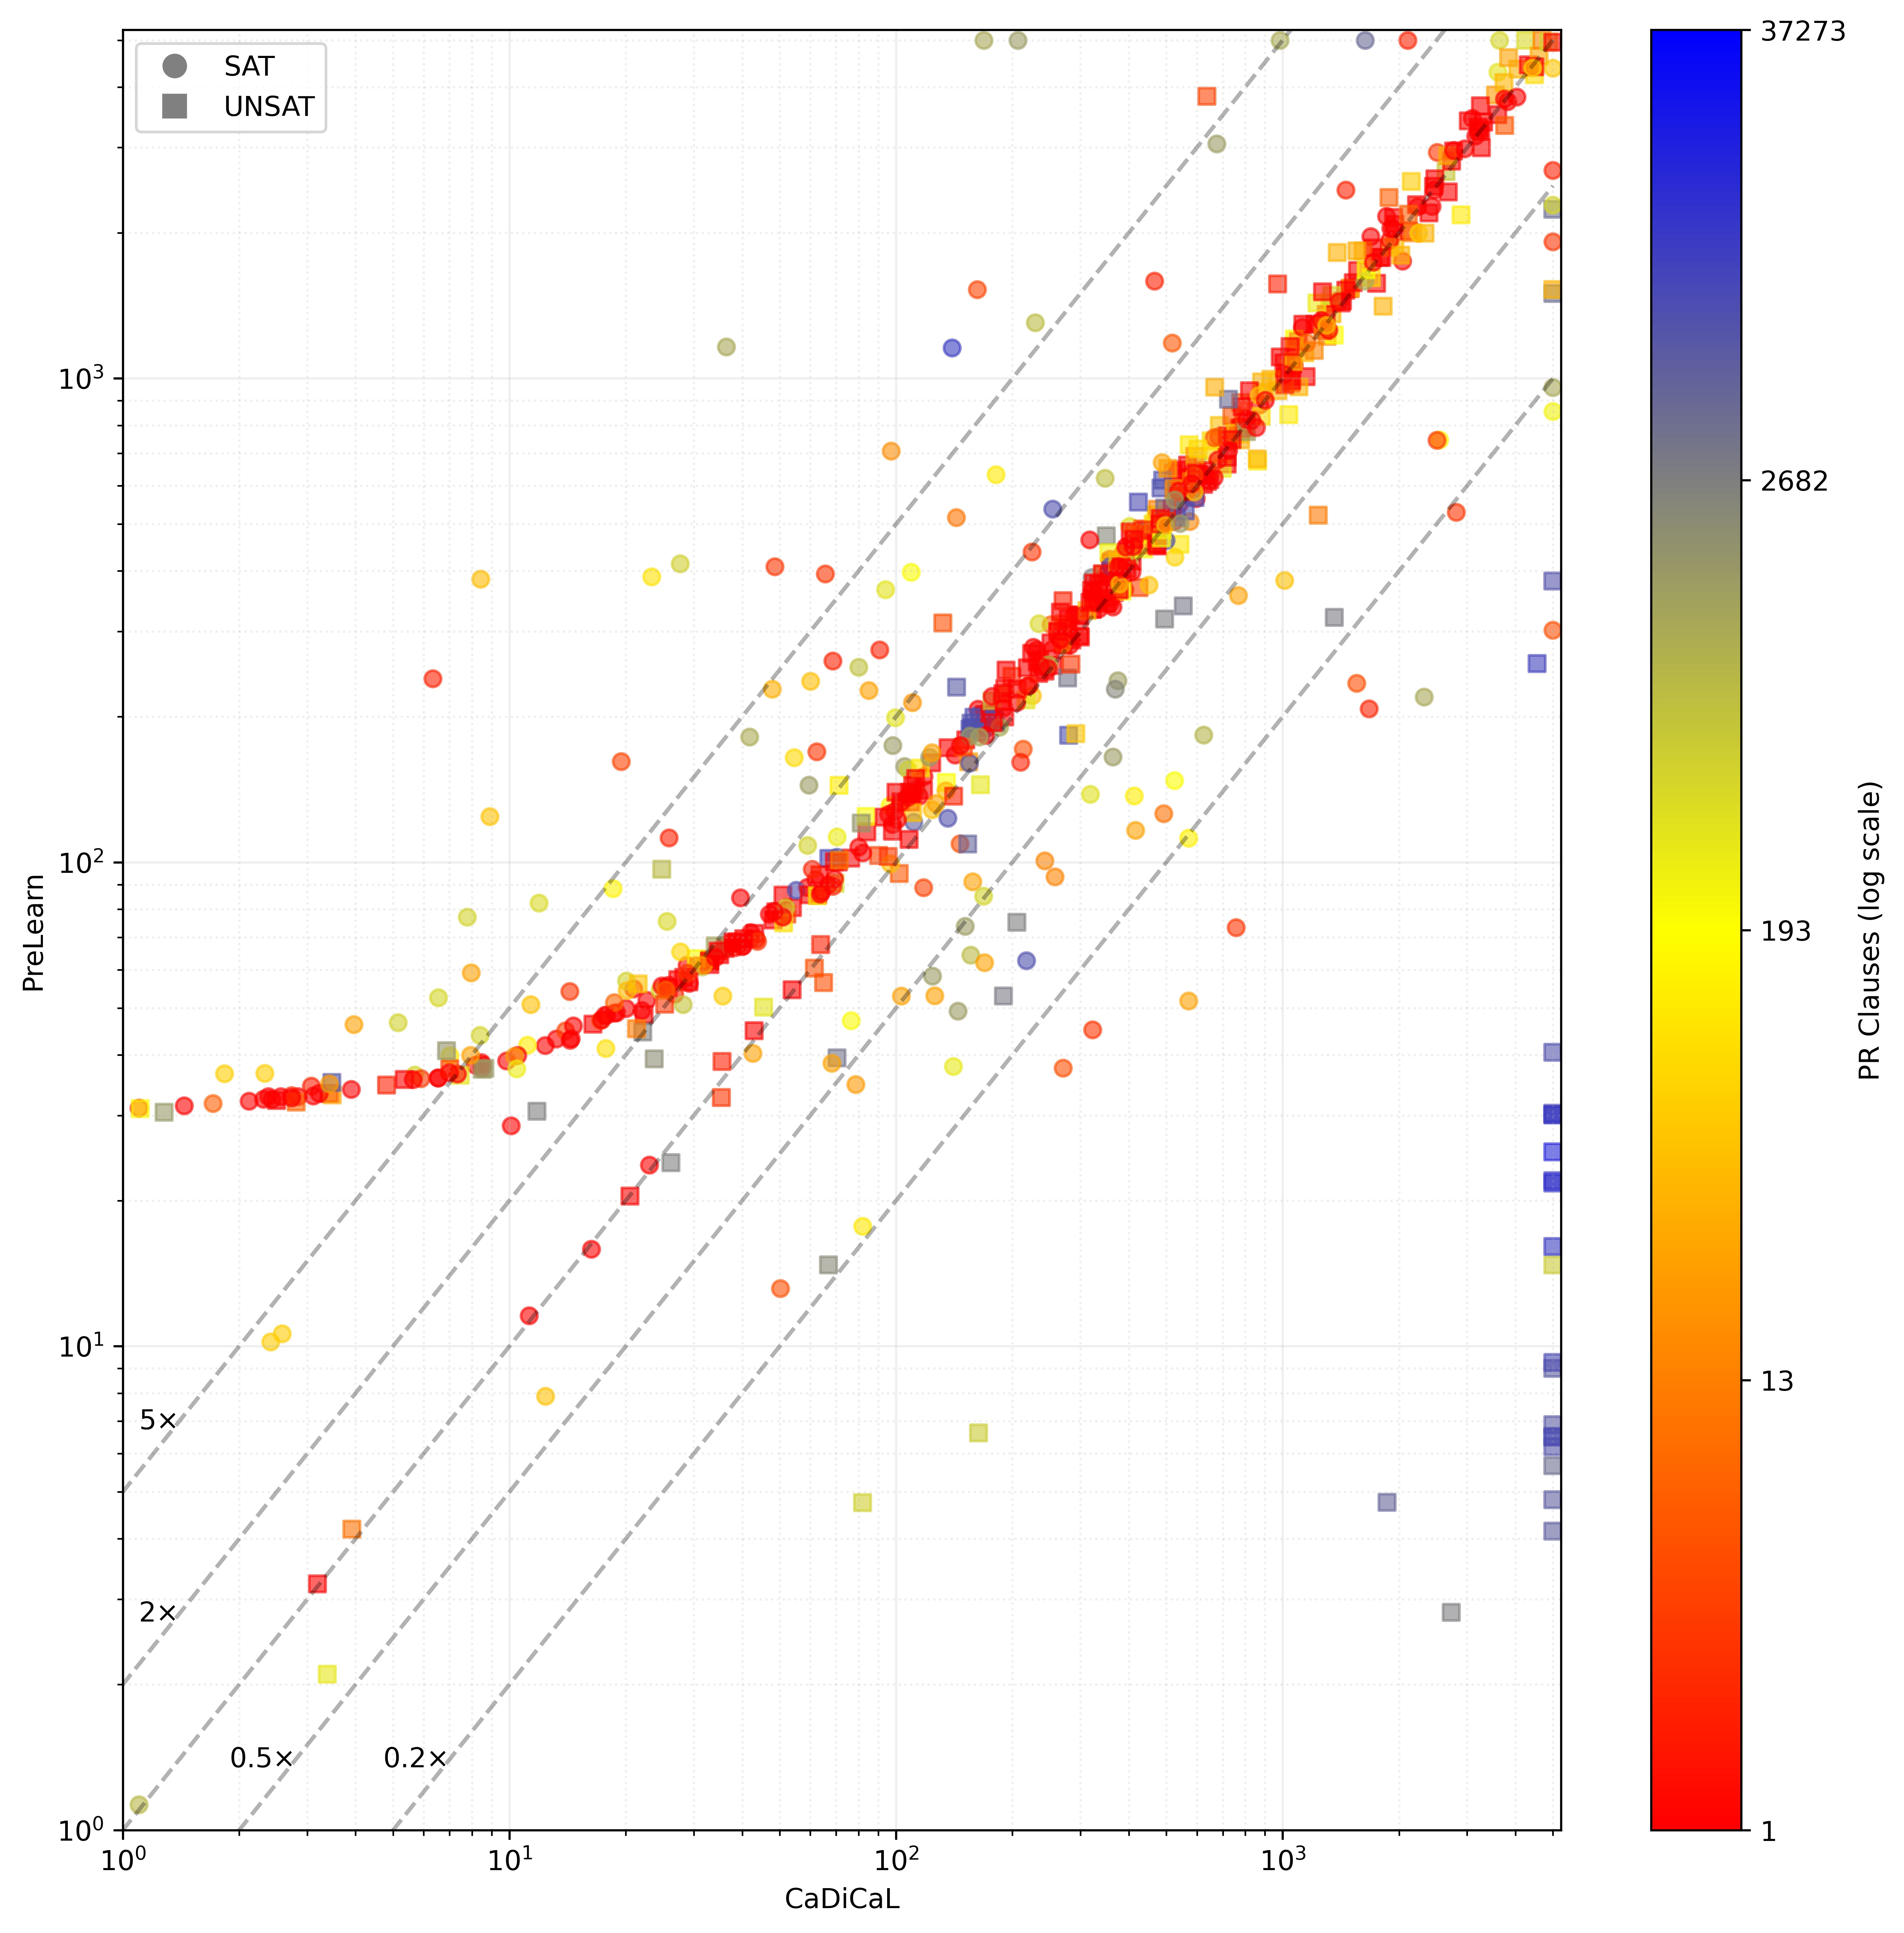
\includegraphics[width=\textwidth]{figs/cadical_vs_prelearn.jpg}
        \caption{Comparison with \prelearn}
        \label{fig:cautical-vs-prelearn}
    \end{subfigure}
    \caption{Performance comparison of \tool with other solvers}
    \label{fig:solver-comparison}
\end{figure*}

In \autoref{fig:solver-comparison}, we compare the performance of \tool with \cadical and \prelearn on the benchmarks from the '22,'23, and '24 SAT competition's main tracks. \autoref{tab:solver-stats} shows the number of instances solved by each solver as well as the number of queries for which \prelearn and \cadical learn additional clauses, improve upon \cadical, and solve that \cadical does not solve.

The PAR-2 score is used to evaluate the performance of the solvers at the competition, it is the sum of the runtime on instances solved plus two times the timeout for each instance unsolved. On this dataset, \cadical has a PAR-score of 3521.79 seconds, \prelearn has a PAR-score of 3331.41 seconds, and \tool has a PAR-score of 3442.14 seconds.

% prelearn PAR score:  3331.406813590451
% cautical PAR score:  3442.137998163452
% cadical PAR score:  3521.7908356290172

\begin{table}[ht]
    \centering
    \sisetup{table-format=3}        % remove if you are not using siunitx
    \begin{tabular}{lrrrr}
      \toprule
      & \multicolumn{2}{c}{0--10k} & \multicolumn{2}{c}{10k--20M} \\
      \cmidrule(lr){2-3} \cmidrule(lr){4-5}
      & SAT & UNSAT & SAT & UNSAT \\
      \midrule
      \cadical Solved      &  54 &  73 & 354 & 349 \\
      \midrule
      \prelearn \\
      \; Total &  52 &  92 & 356 & 355 \\
      \; Learnt clauses   &  43 &  75 & 216 & 203 \\
      \; Improved &  12 &  31 &  32 &  22 \\
      \; Exclusively &   1 &  19 &   6 &   9 \\
      \midrule
      \tool \\
      \; Total &  52 &  87 & 349 & 327 \\
      \; Learnt clauses     &  16 &  59 &  32 &  36 \\
      \; Improved &  23 &  33 &  87 &  78 \\
      \; Exclusively &   0 &  18 &   9 &   9 \\
      \bottomrule
    \end{tabular}
    \caption{Number of solved instances.}
    \label{tab:solver-stats}
  \end{table}





  % todo : update these numbers

\subsection{Discussion of Benchmark Families}~\label{subsec:eval-discussion}

We identify six benchmark families, which \pr clauses  based on prior work ~\cite{prelearn} and our experiments on SATCOMP benchmarks:

\begin{enumerate}
    \item \texttt{mutilated-chessboard}
    \item 
    \item 
    \item 
    \item 
    \item 
    \item 
    \item 
\end{enumerate}

\begin{figure*}[!t]
    \centering
    \begin{subfigure}[t]{0.3\textwidth}
            \centering
            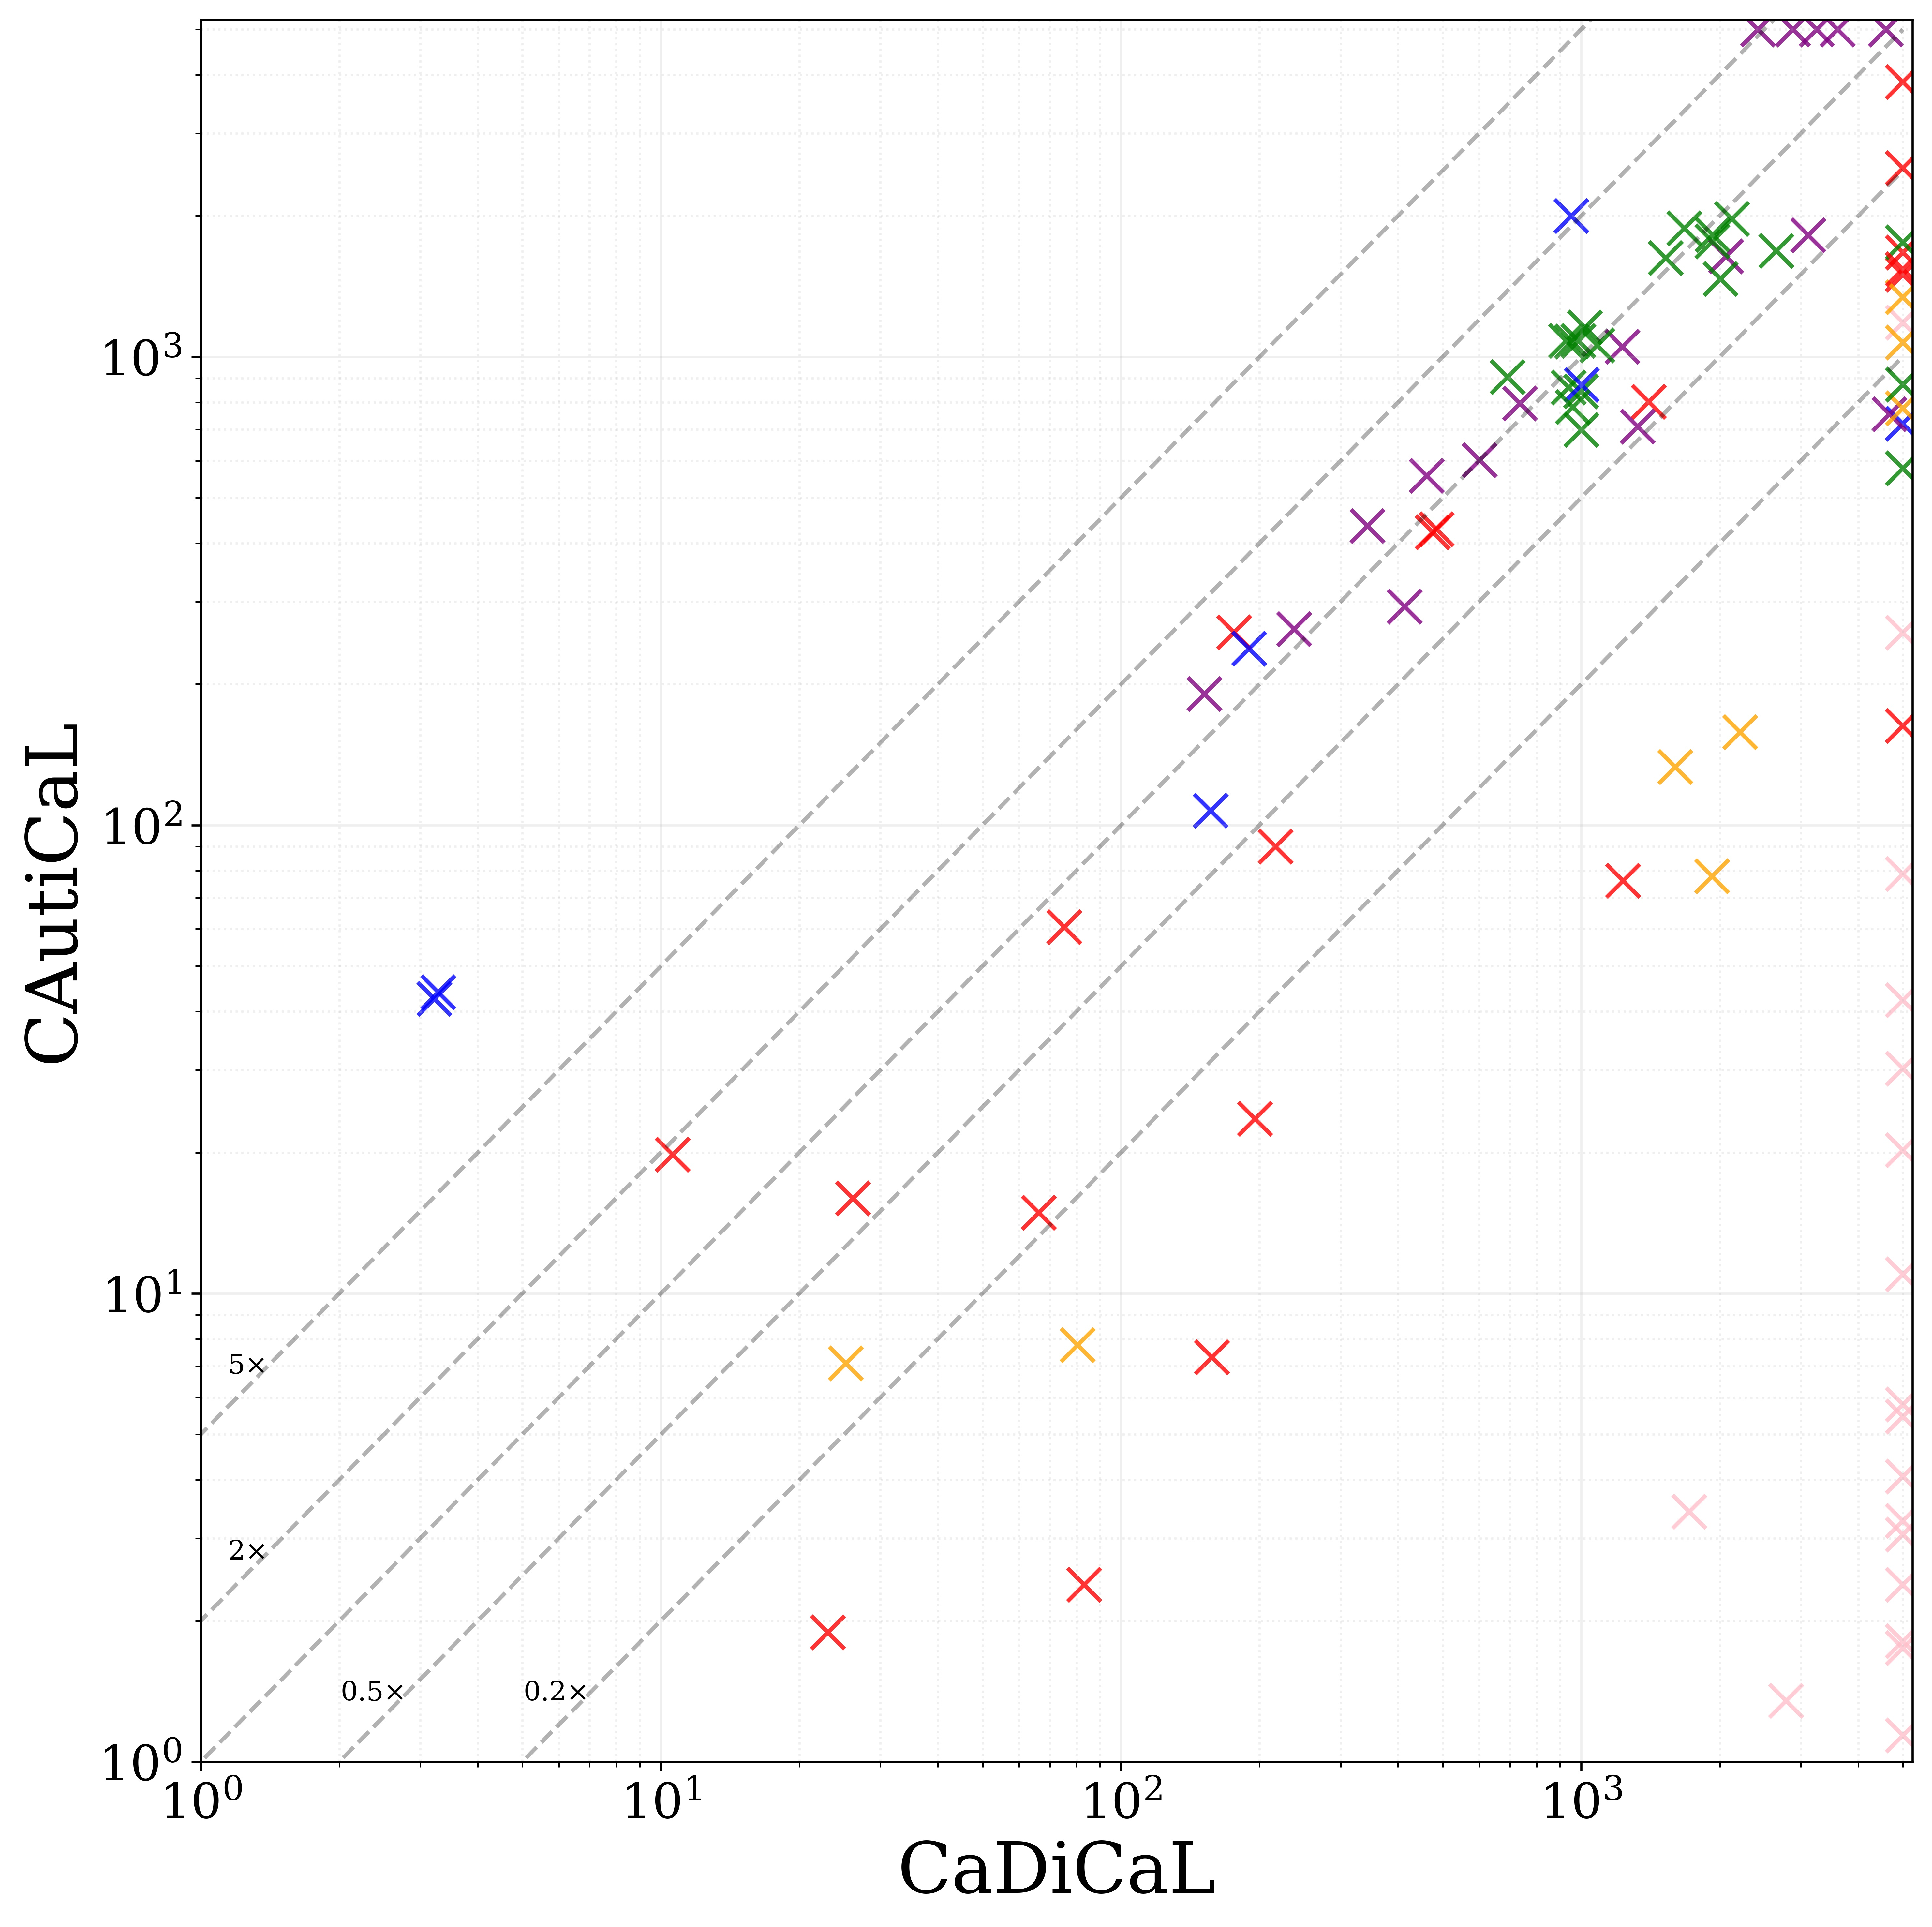
\includegraphics[width=\textwidth]{figs/cadical_vs_cautical_interesting.jpg}
            \caption{Comparison with \cadical}
            \label{fig:cautical-vs-cadical}
    \end{subfigure}
        % \hspace{0.06\textwidth}
    % \hspace{0.06\textwidth}
    \begin{subfigure}[t]{0.3\textwidth}
        \centering
        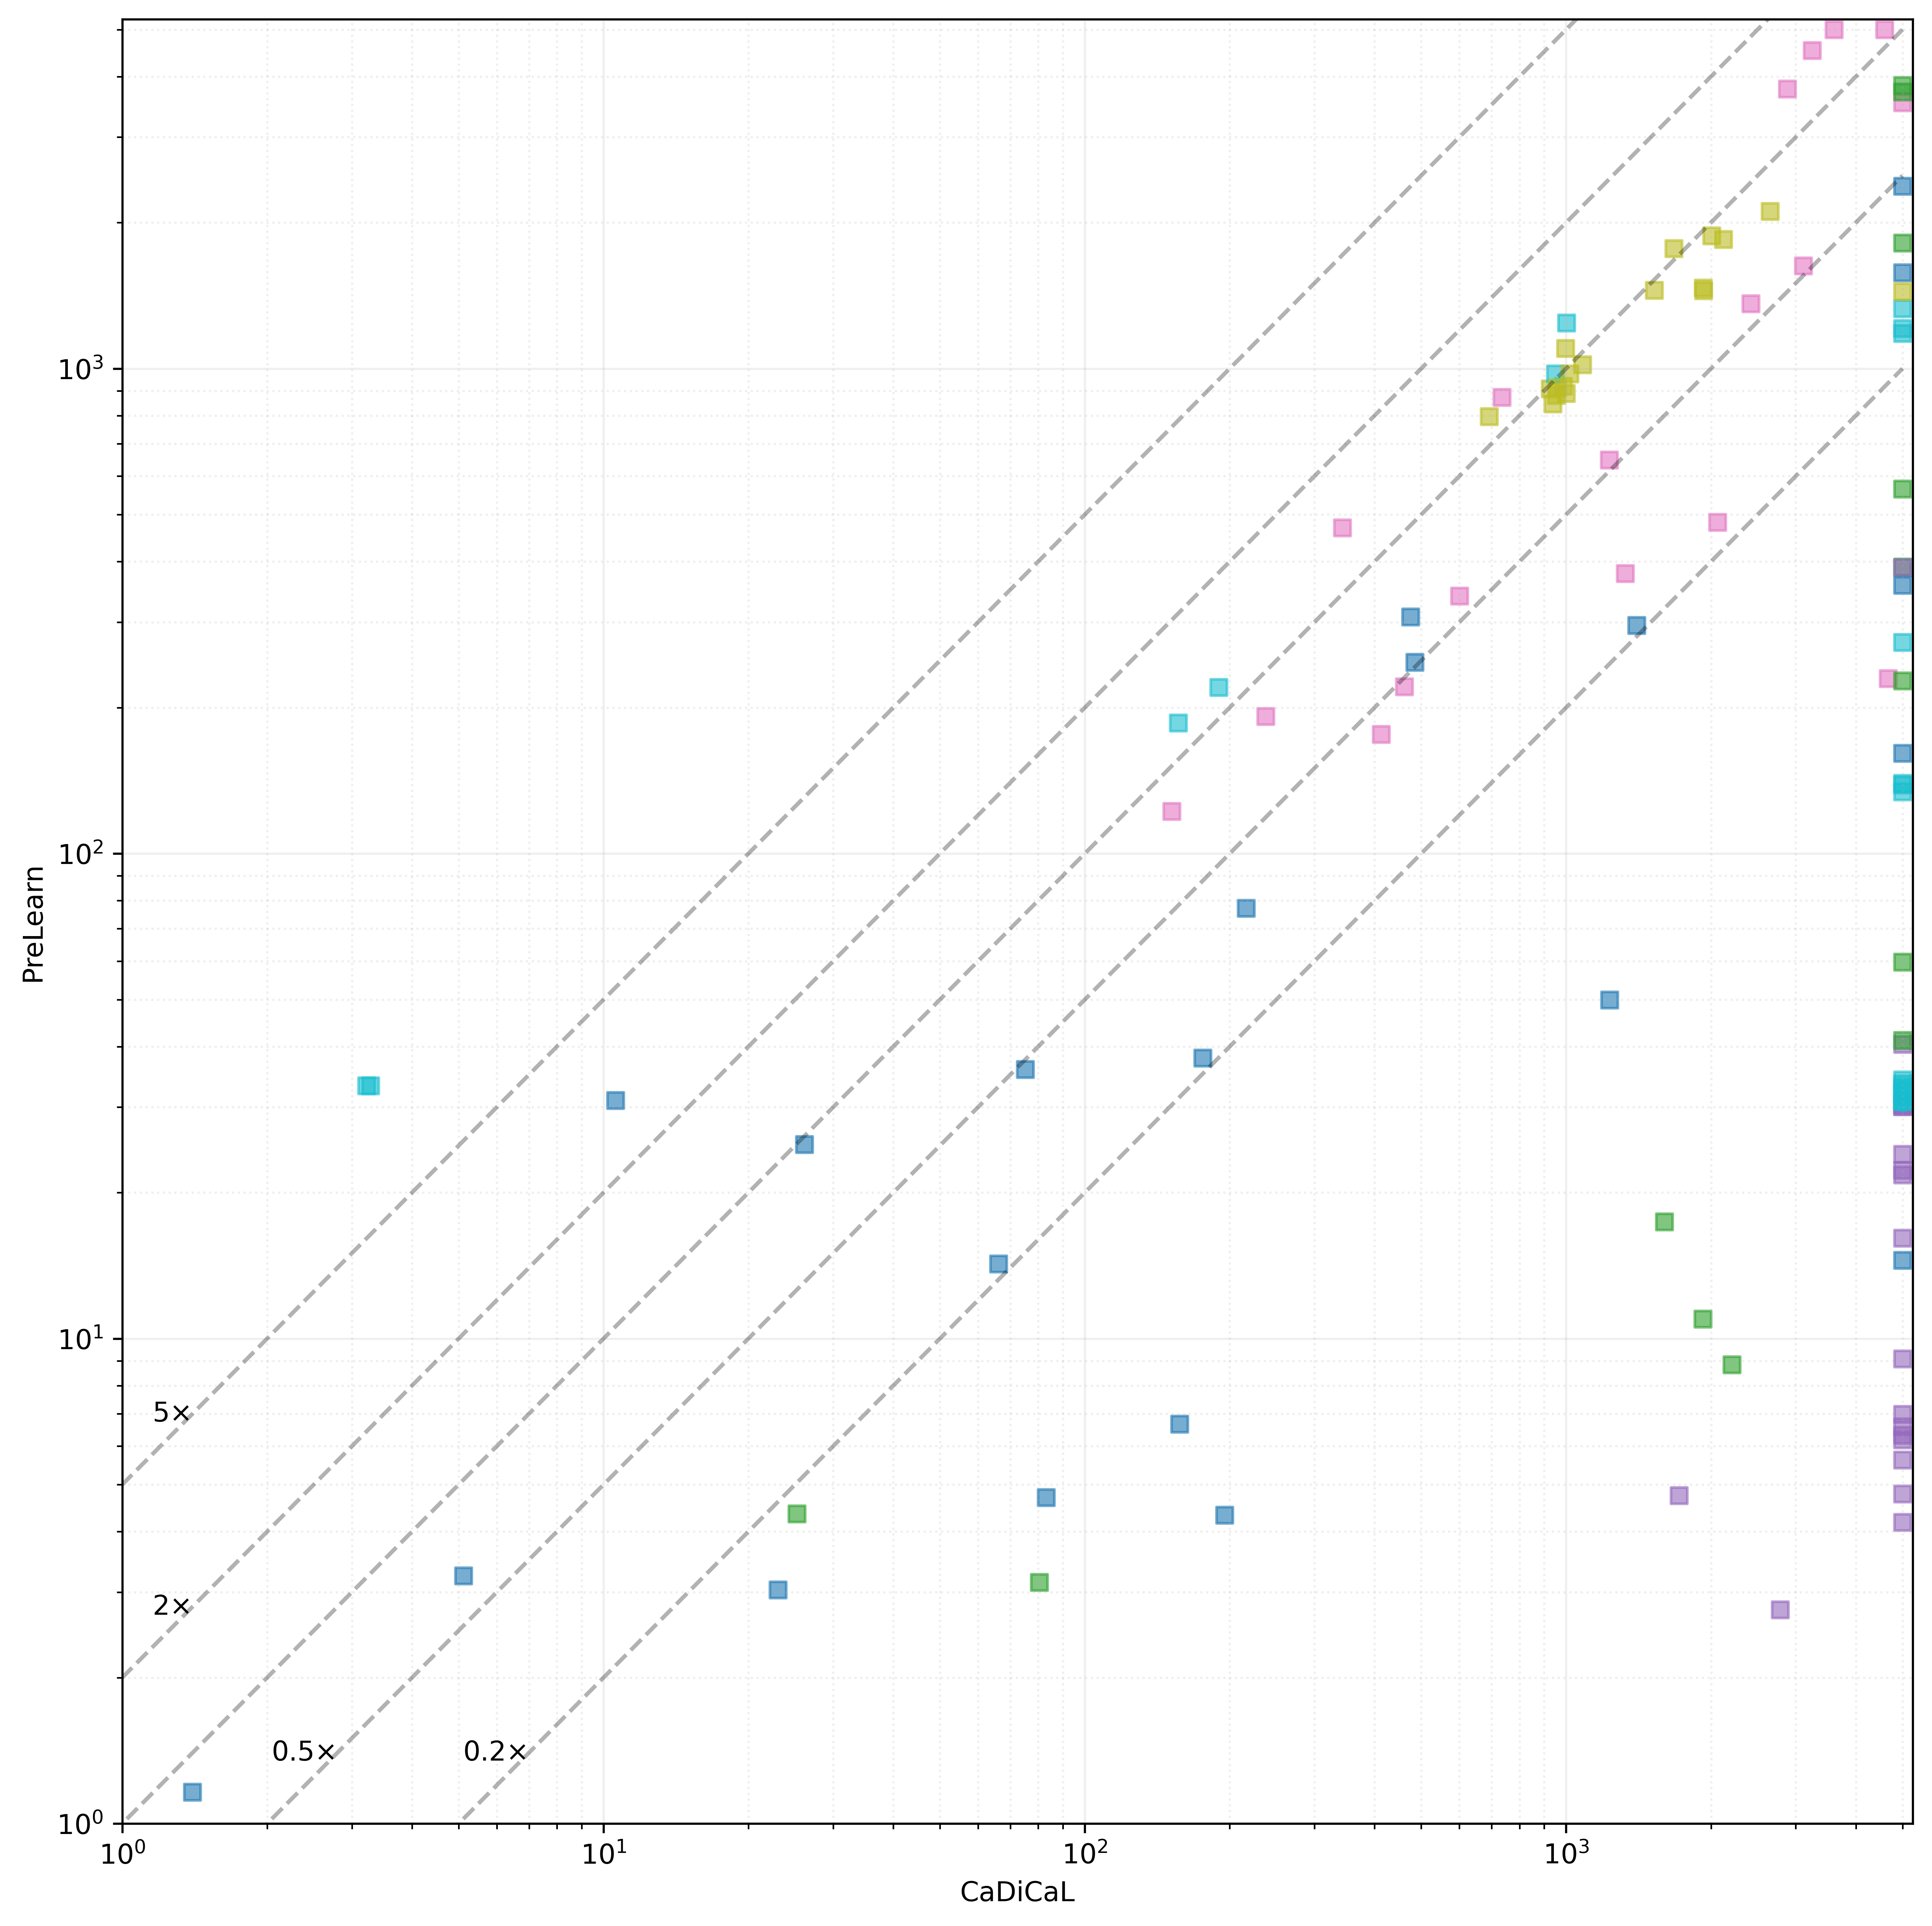
\includegraphics[width=\textwidth]{figs/prelearn_vs_cadical_interesting.jpg}
        \caption{Comparison with \prelearn}
        \label{fig:cautical-vs-prelearn}
    \end{subfigure}
    \begin{subfigure}[t]{0.3\textwidth}
        \centering
        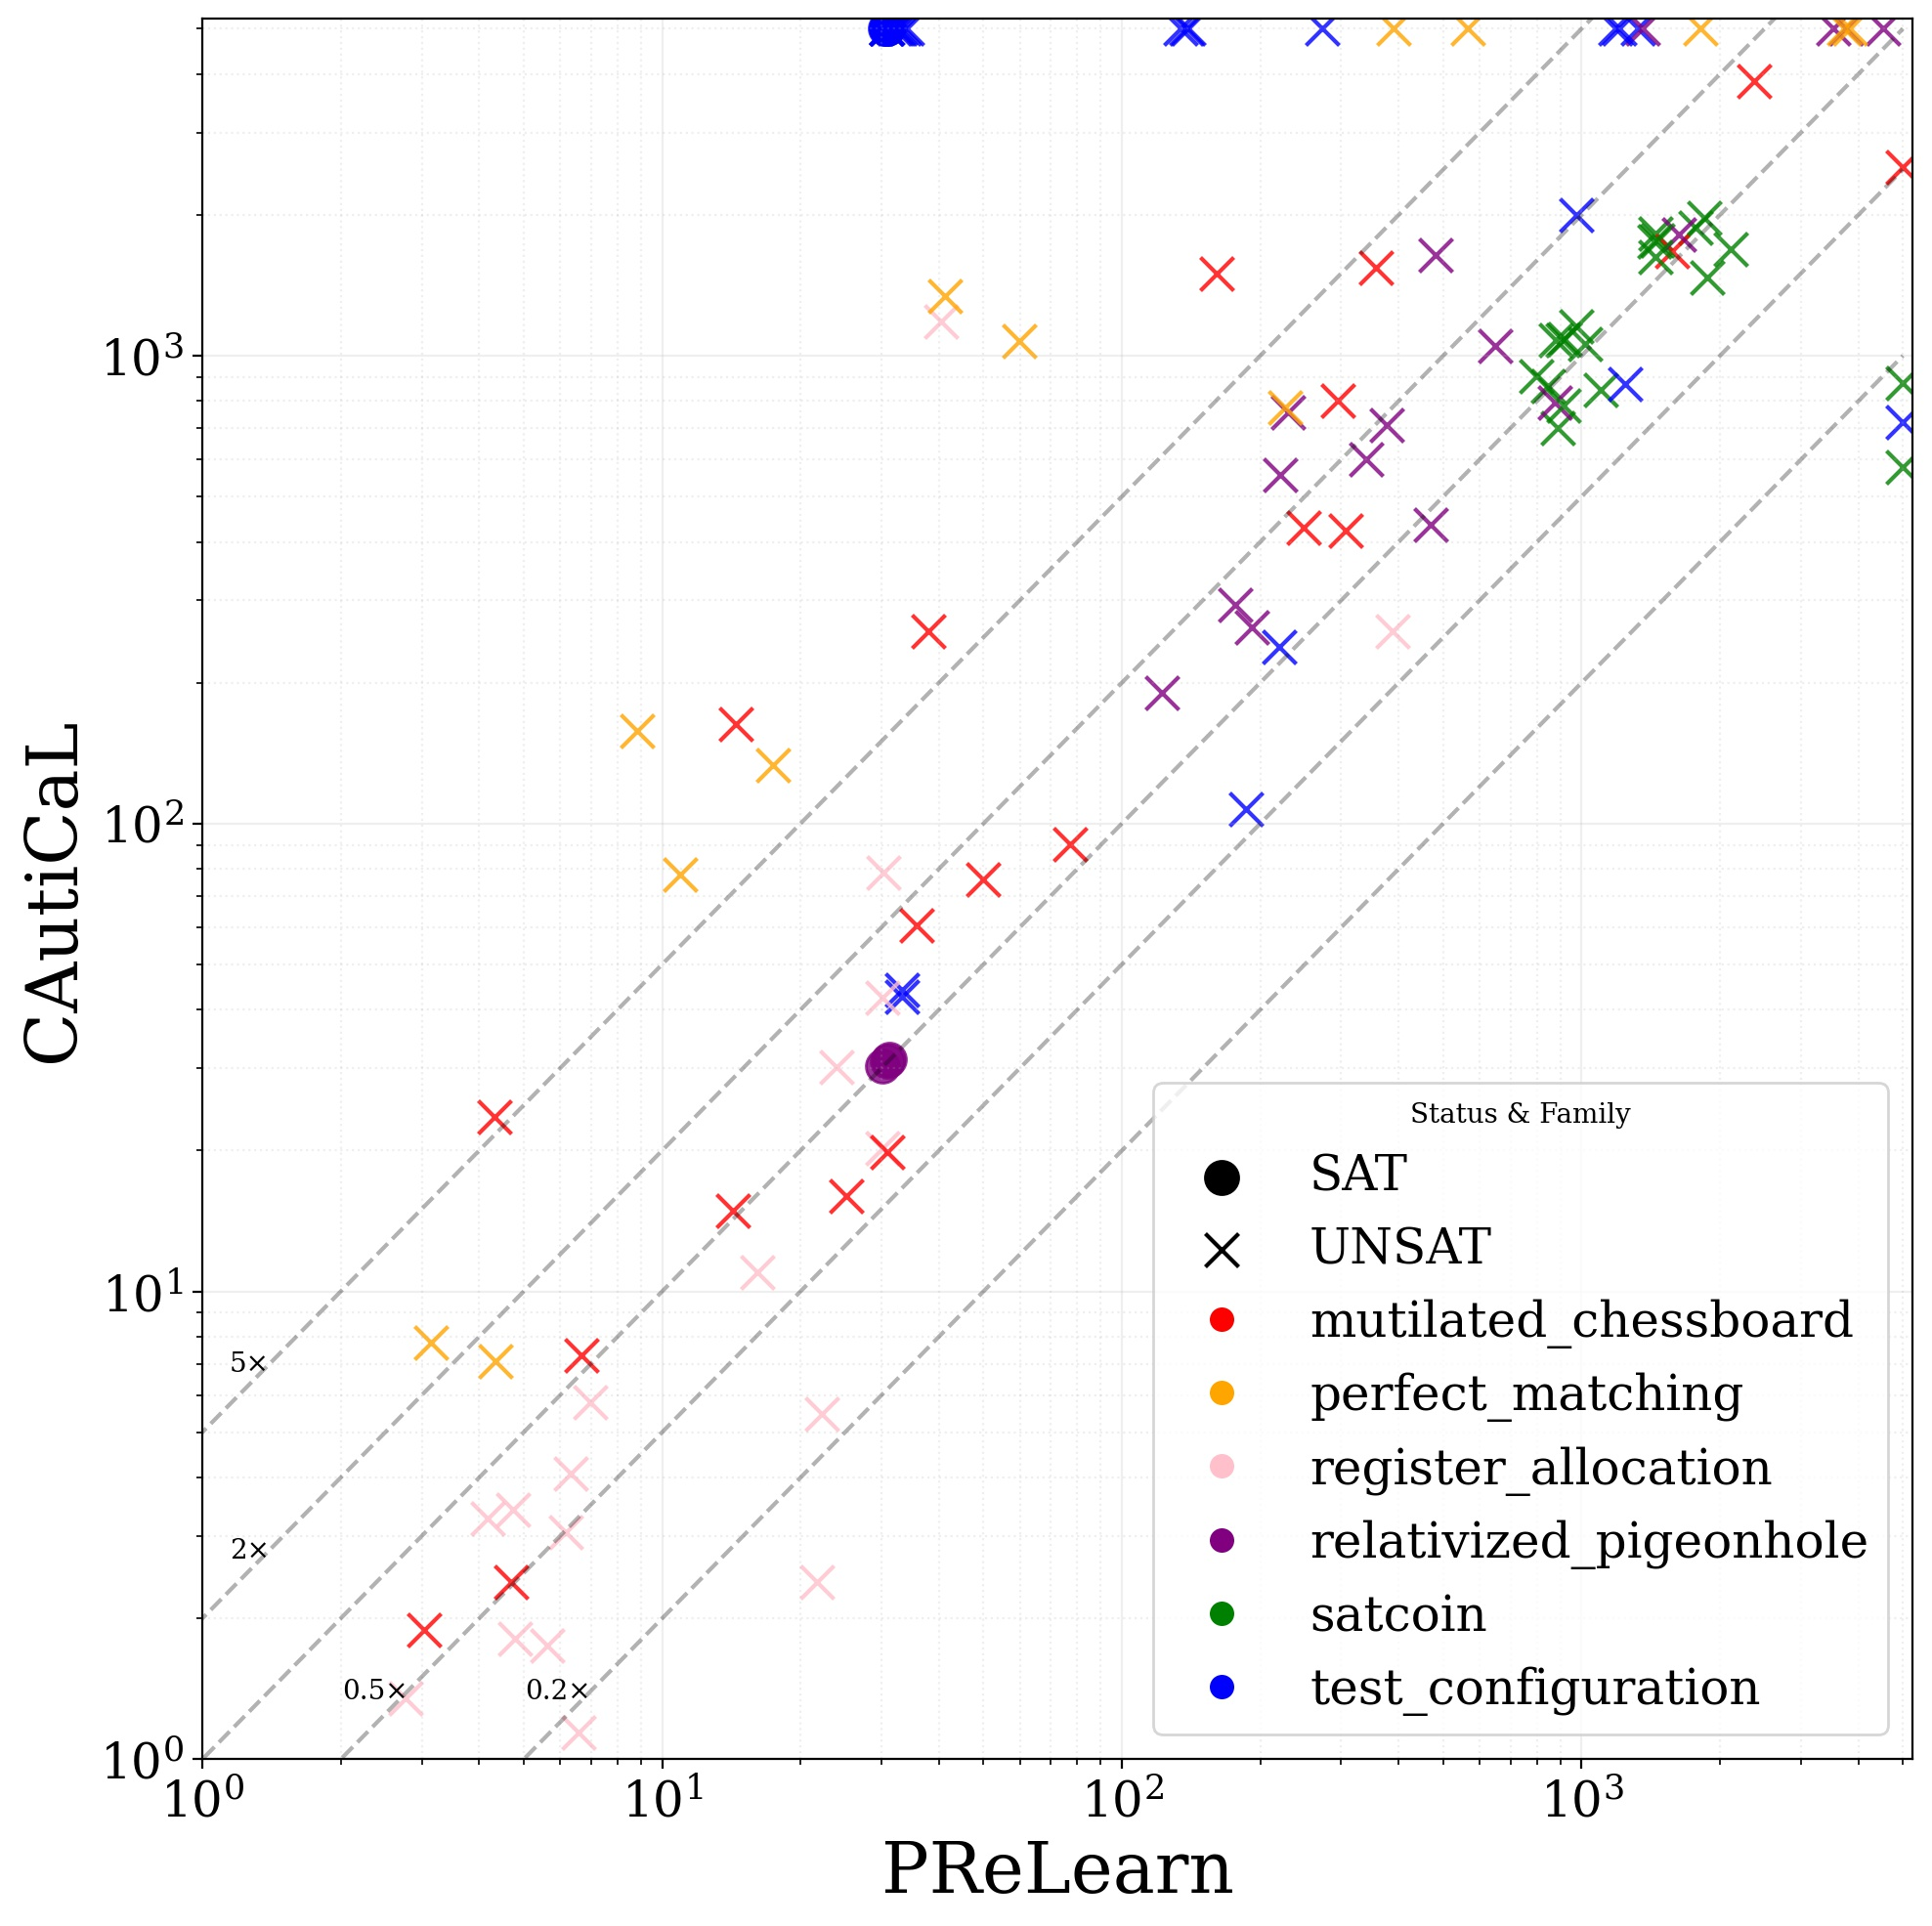
\includegraphics[width=\textwidth]{figs/prelearn_vs_cautical_interesting_legend.jpg}
        \caption{Comparison with \prelearn}
        \label{fig:cautical-vs-prelearn}
    \end{subfigure}

    \caption{Performance comparison of \tool with other solvers}
    \label{fig:solver-comparison}
\end{figure*}





\subsection{Analysis of heuristics}~\label{subsec:eval-heuristics}

We provide a brief analysis of the heuristics used in \tool.


\begin{figure*}[!t]
    \centering
    \begin{subfigure}[t]{0.3\textwidth}
            \centering
            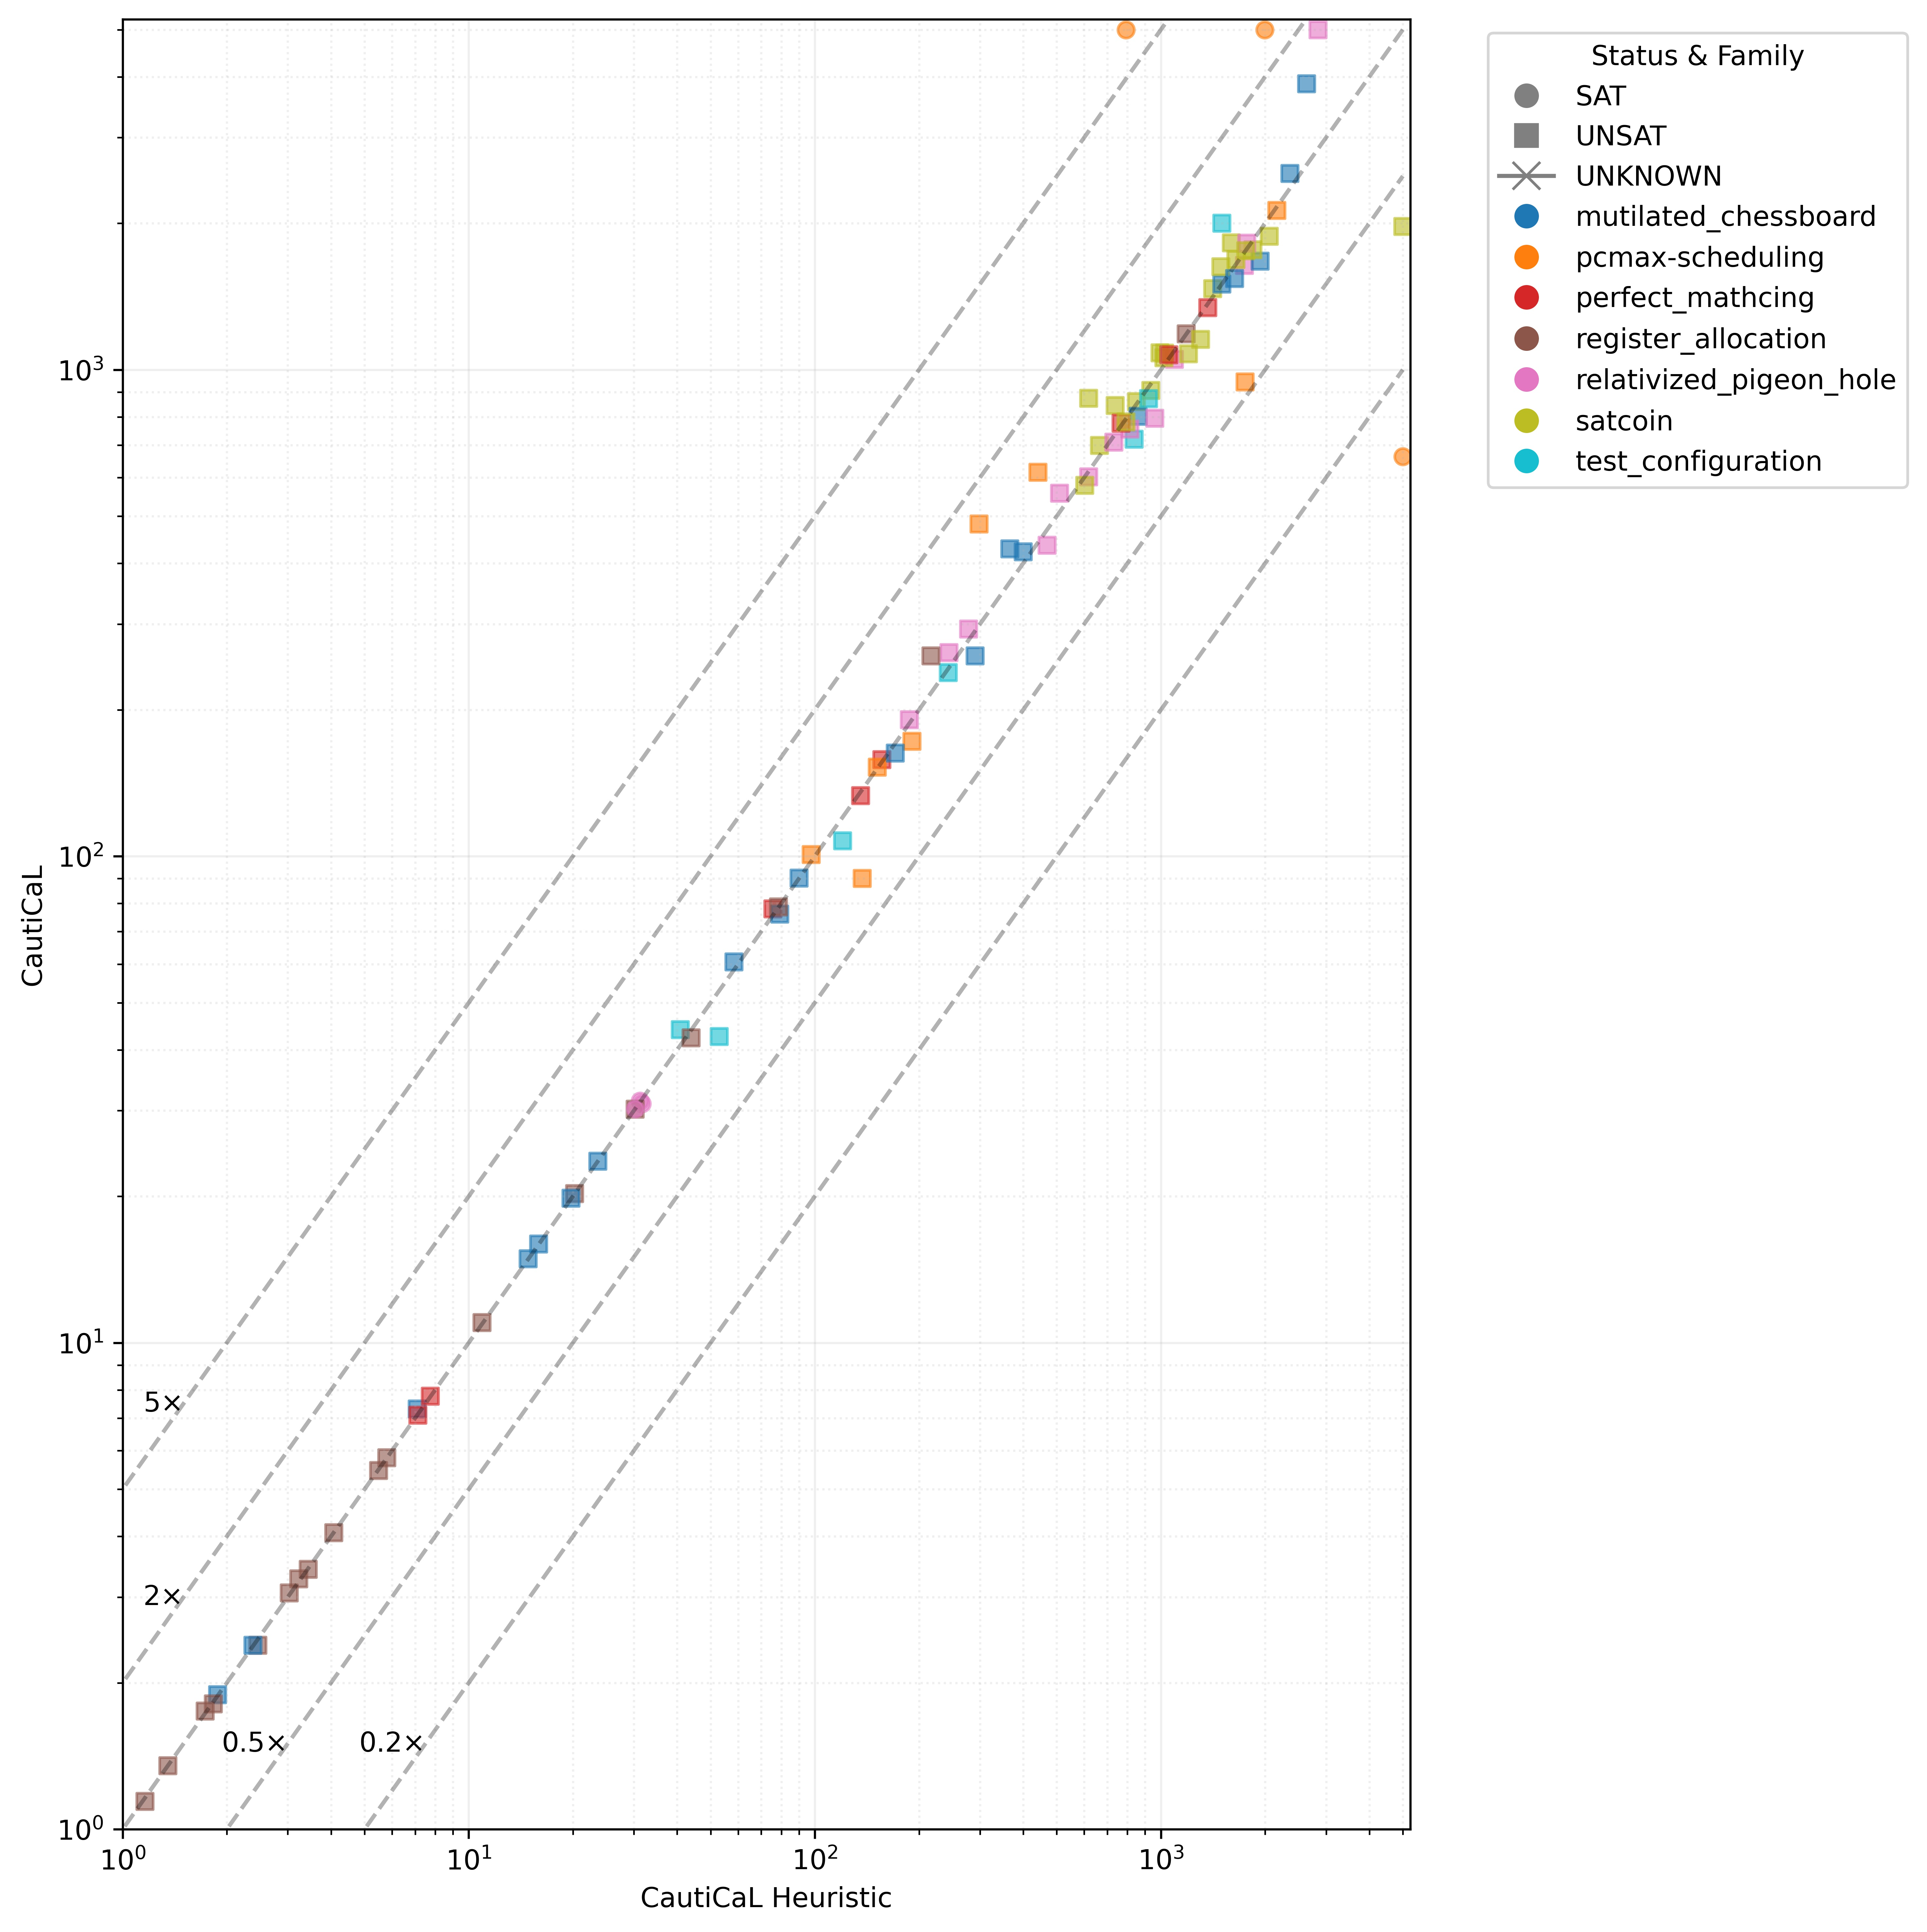
\includegraphics[width=\textwidth]{figs/global_time_lim_heuristic_comparison.jpg}
            \caption{Time limit}
            \label{fig:global-time-comparison}
    \end{subfigure}
        % \hspace{0.06\textwidth}
    % \hspace{0.06\textwidth}
    \begin{subfigure}[t]{0.3\textwidth}
        \centering
        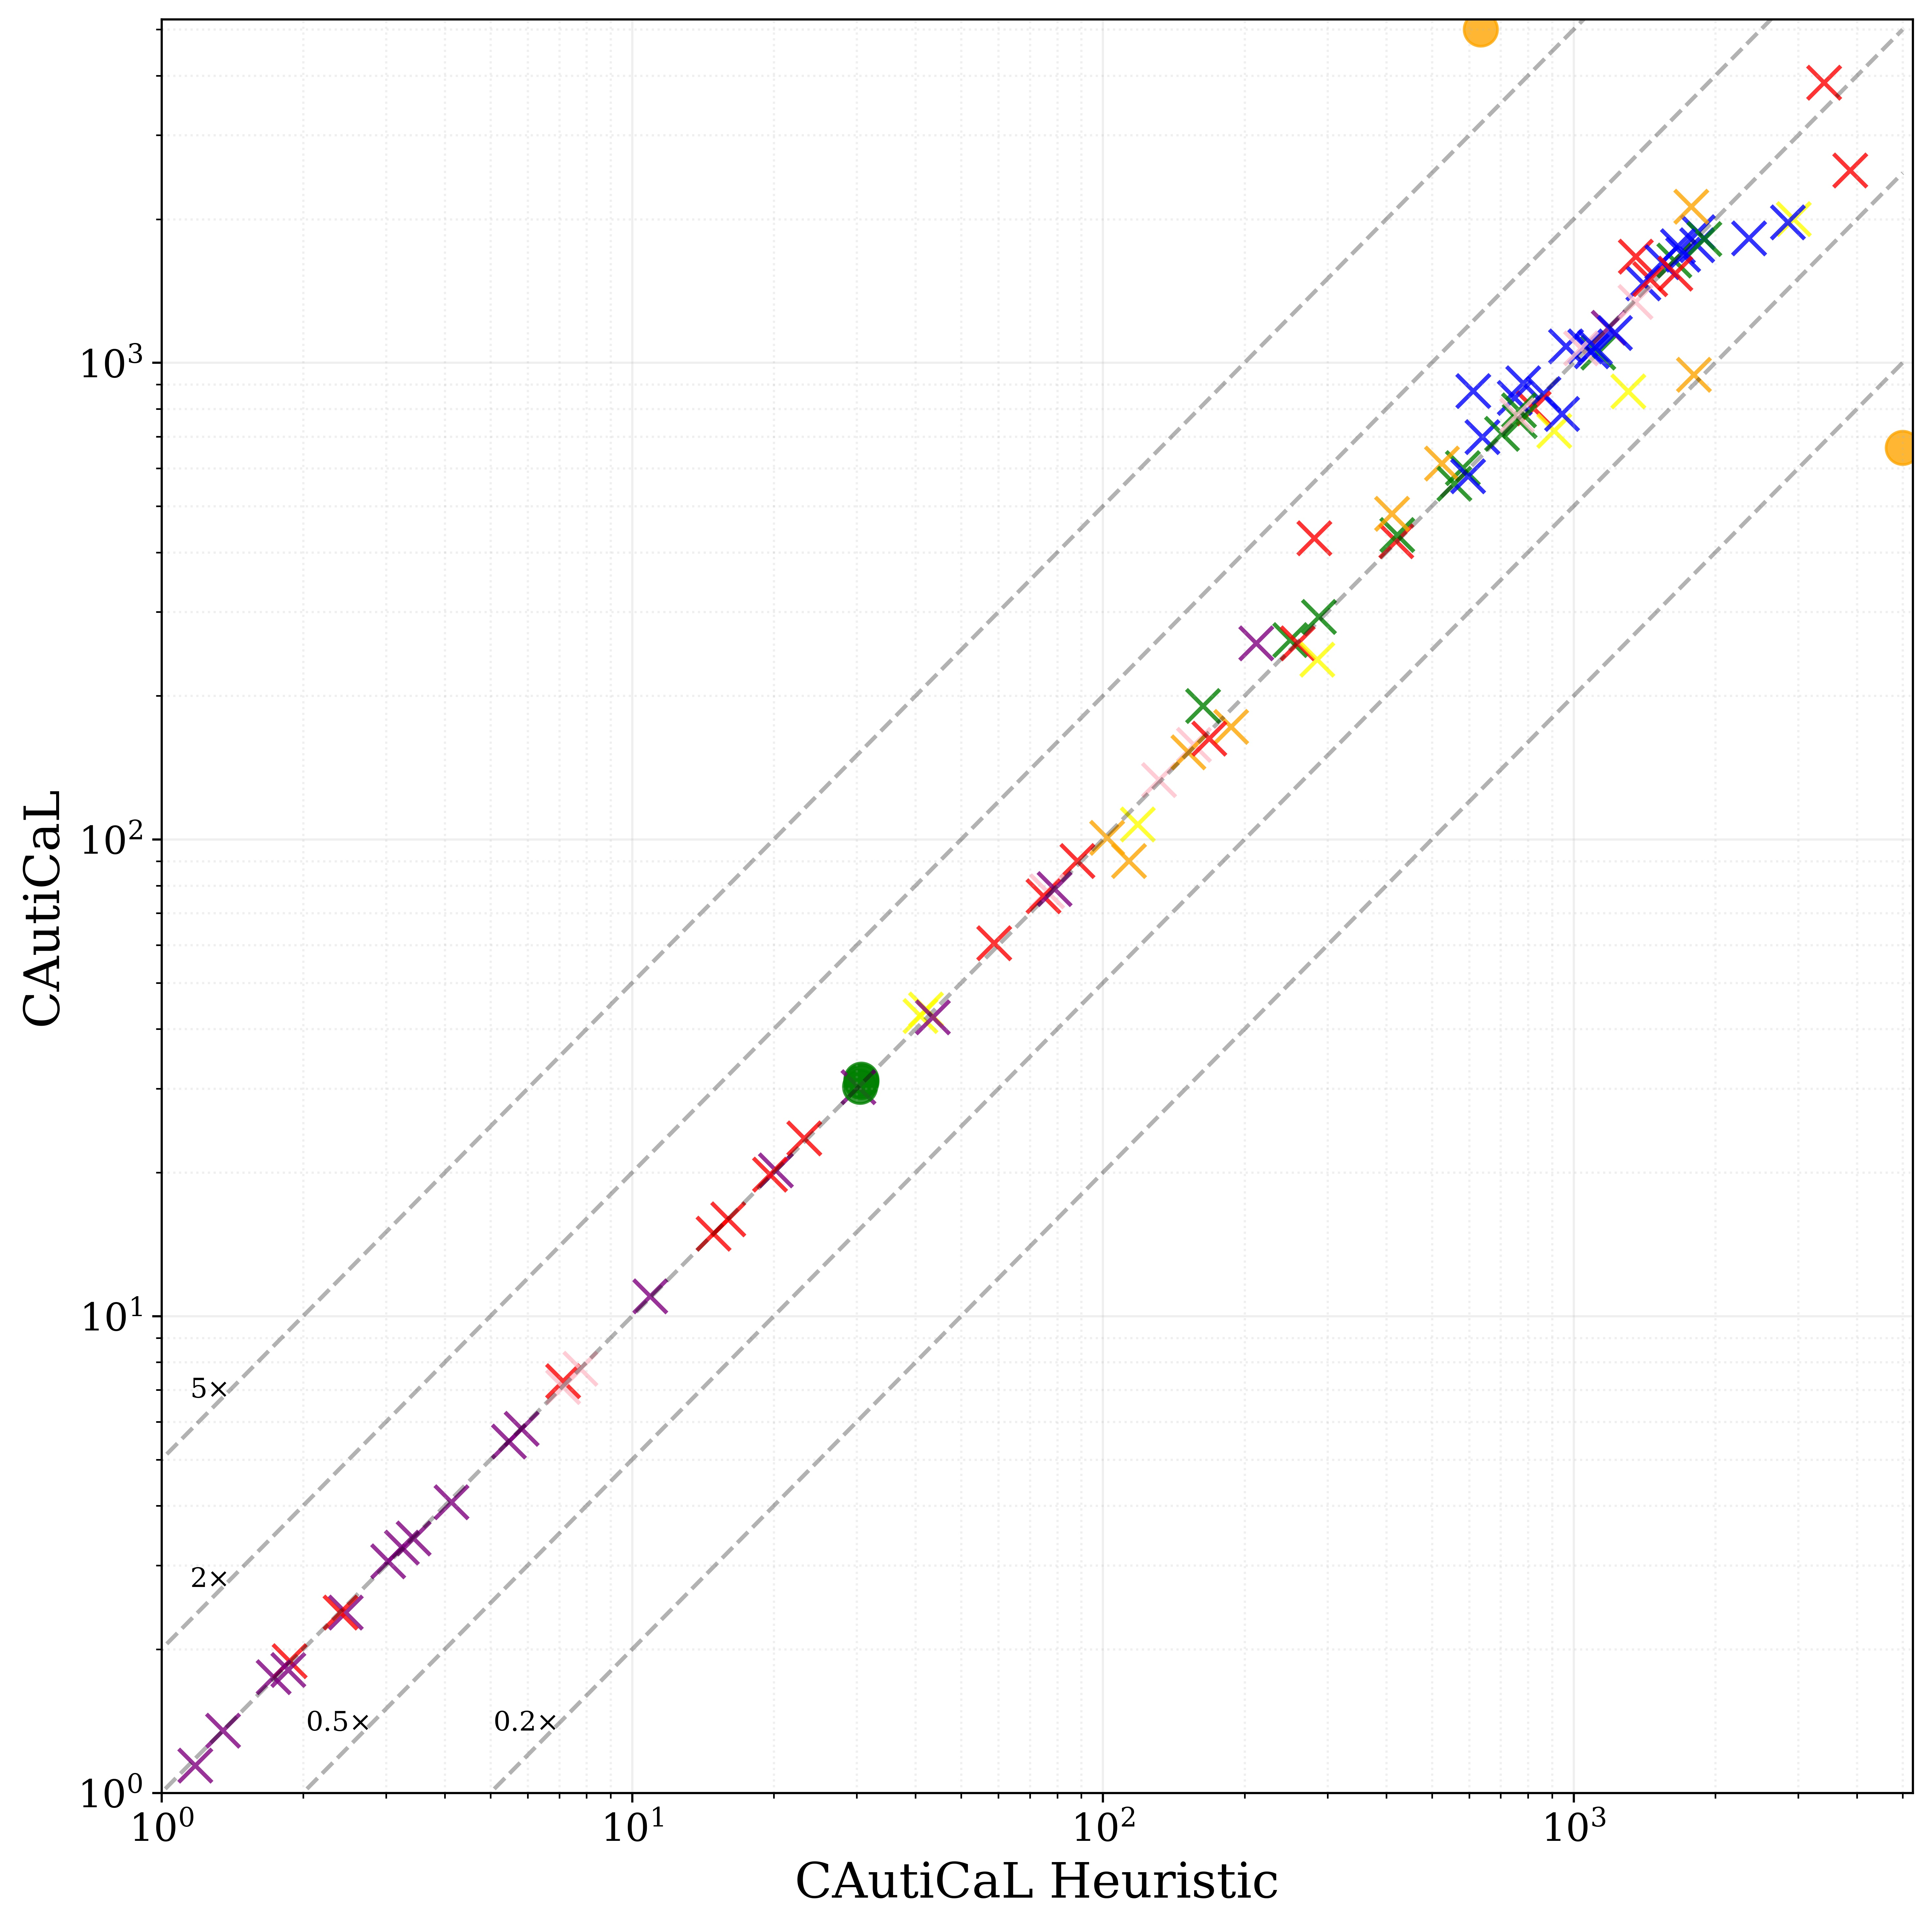
\includegraphics[width=\textwidth]{figs/globalbcp_heuristic_comparison.jpg}
        \caption{BCP}
        \label{fig:globalbcp}
    \end{subfigure}
    \begin{subfigure}[t]{0.3\textwidth}
        \centering
        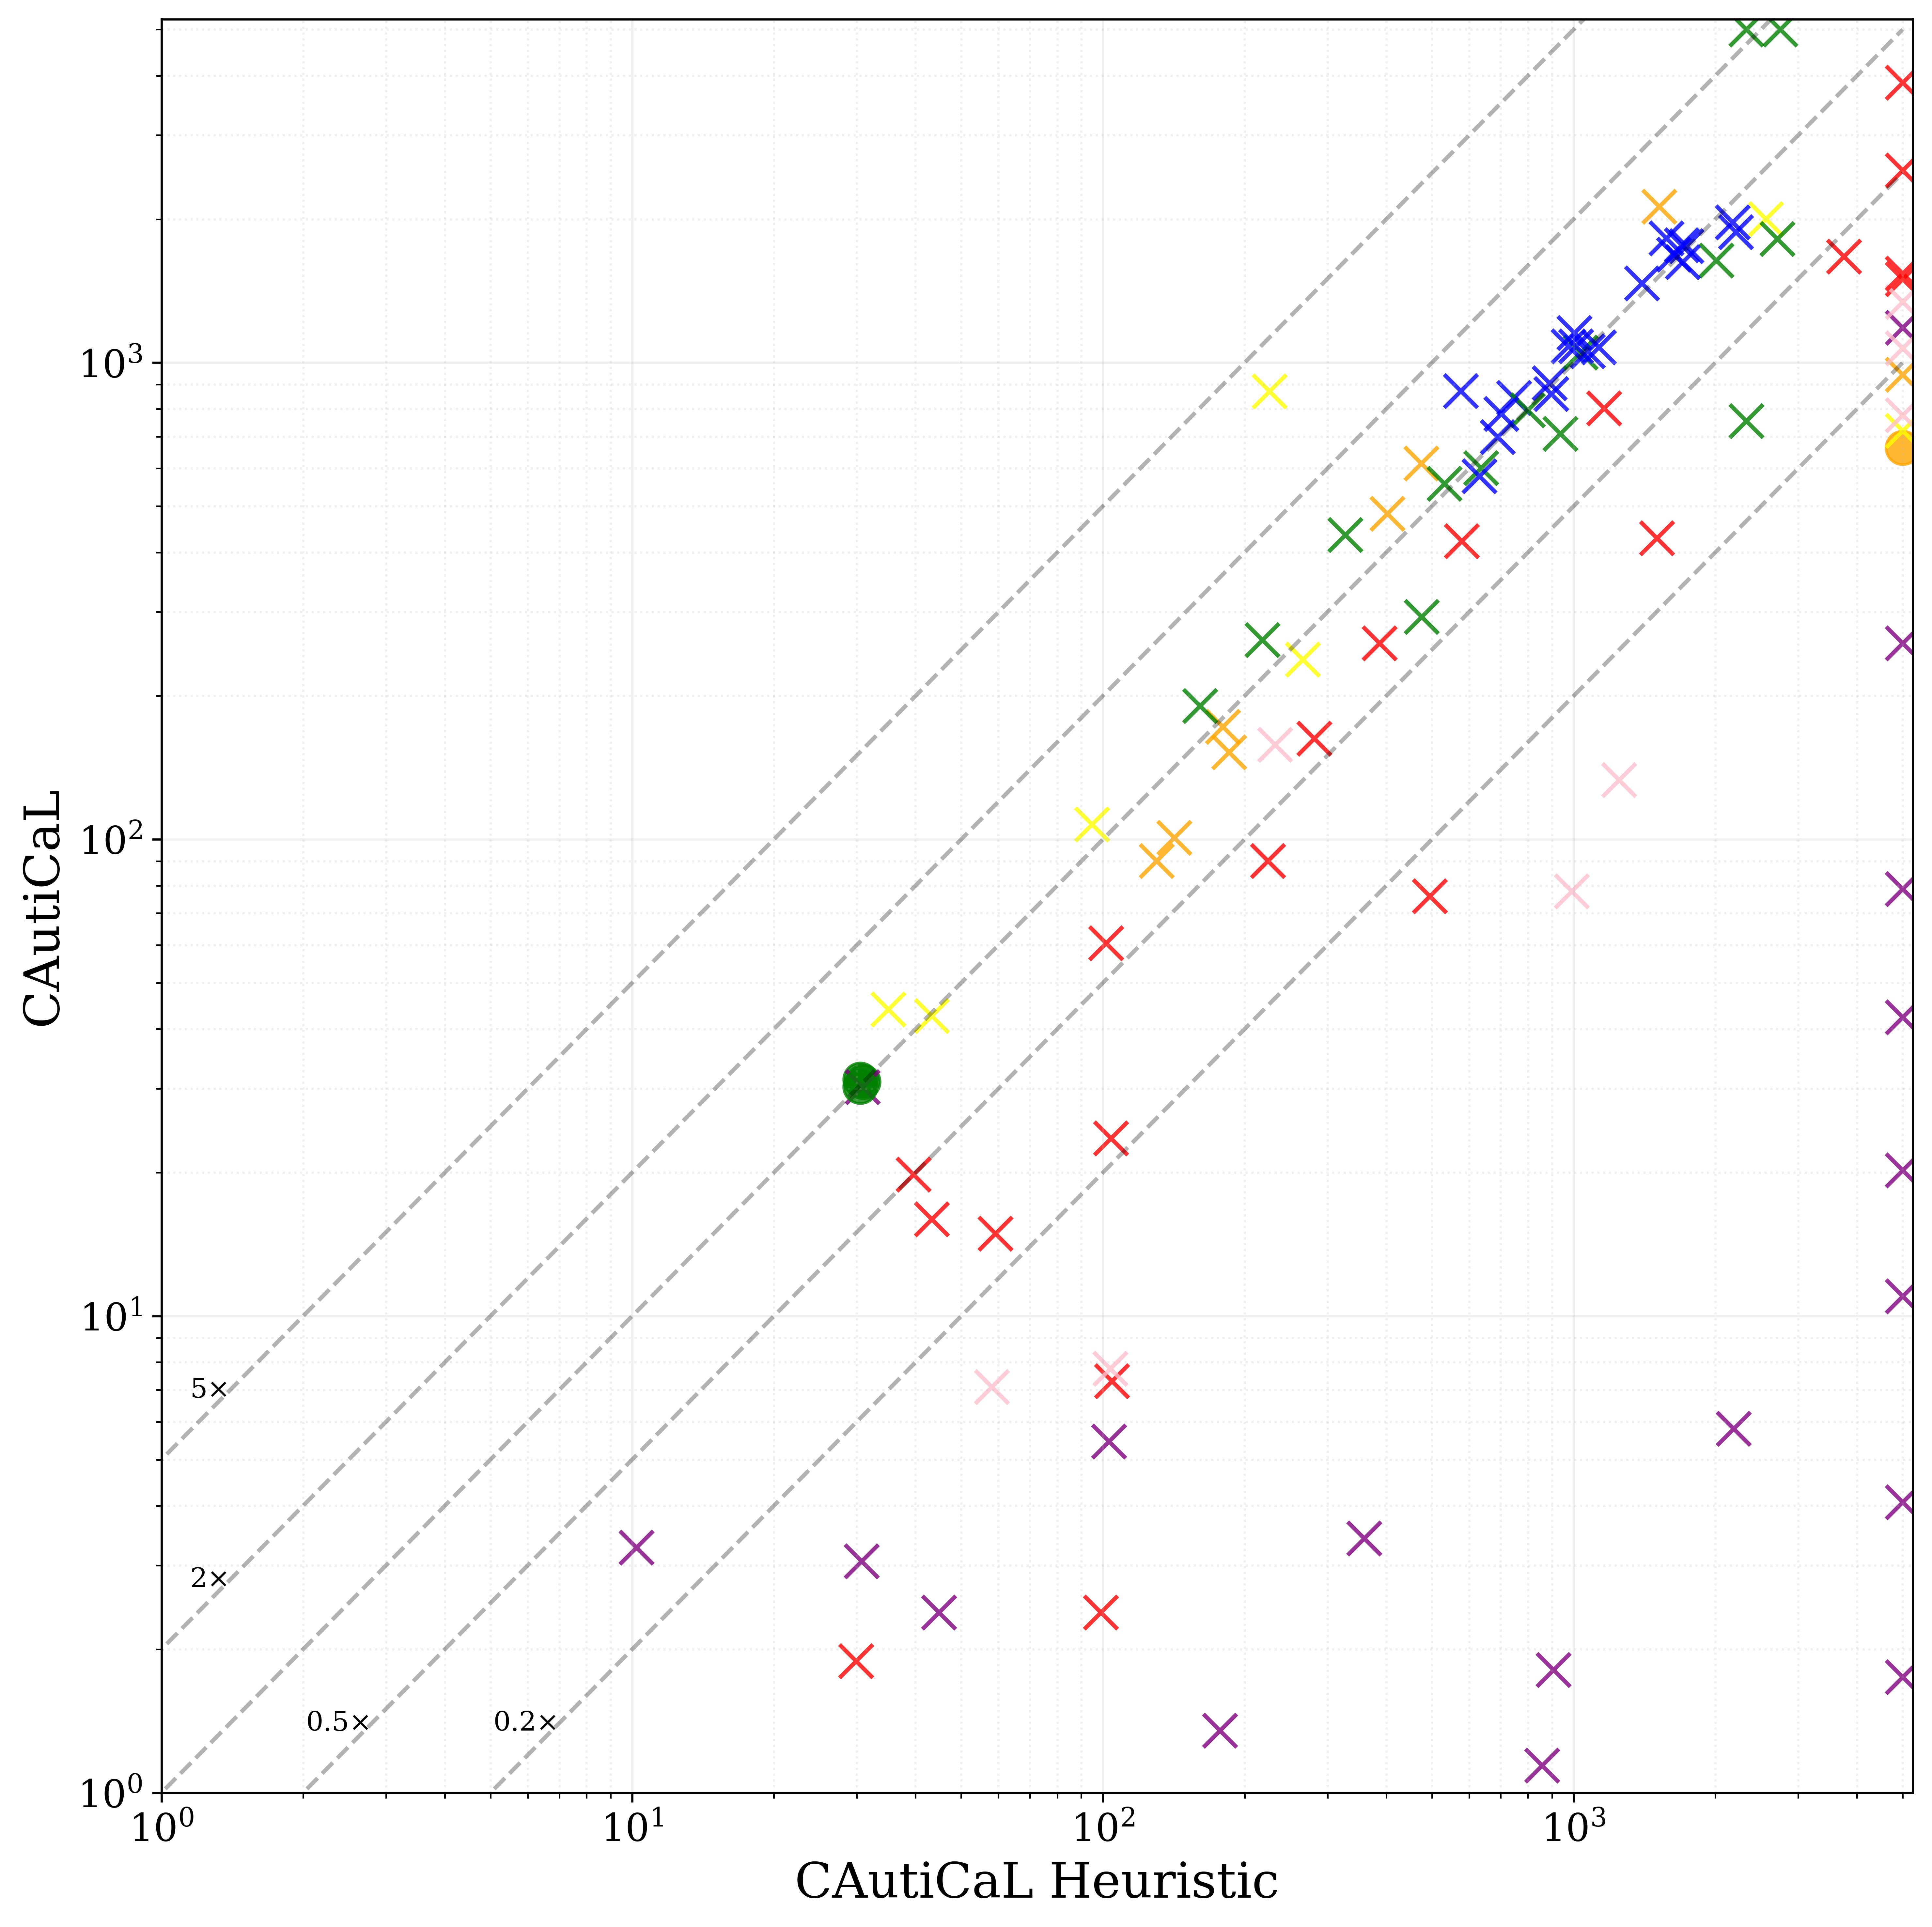
\includegraphics[width=\textwidth]{figs/globaldontfilter_heuristic_comparison.jpg}
        \caption{No filter}
        \label{fig:globaldontfilter}
    \end{subfigure}

    \caption{Performance comparison of \tool with other solvers}
    \label{fig:solver-comparison}
\end{figure*}

\begin{figure*}[!t]
    \centering
    \begin{subfigure}[t]{0.3\textwidth}
            \centering
            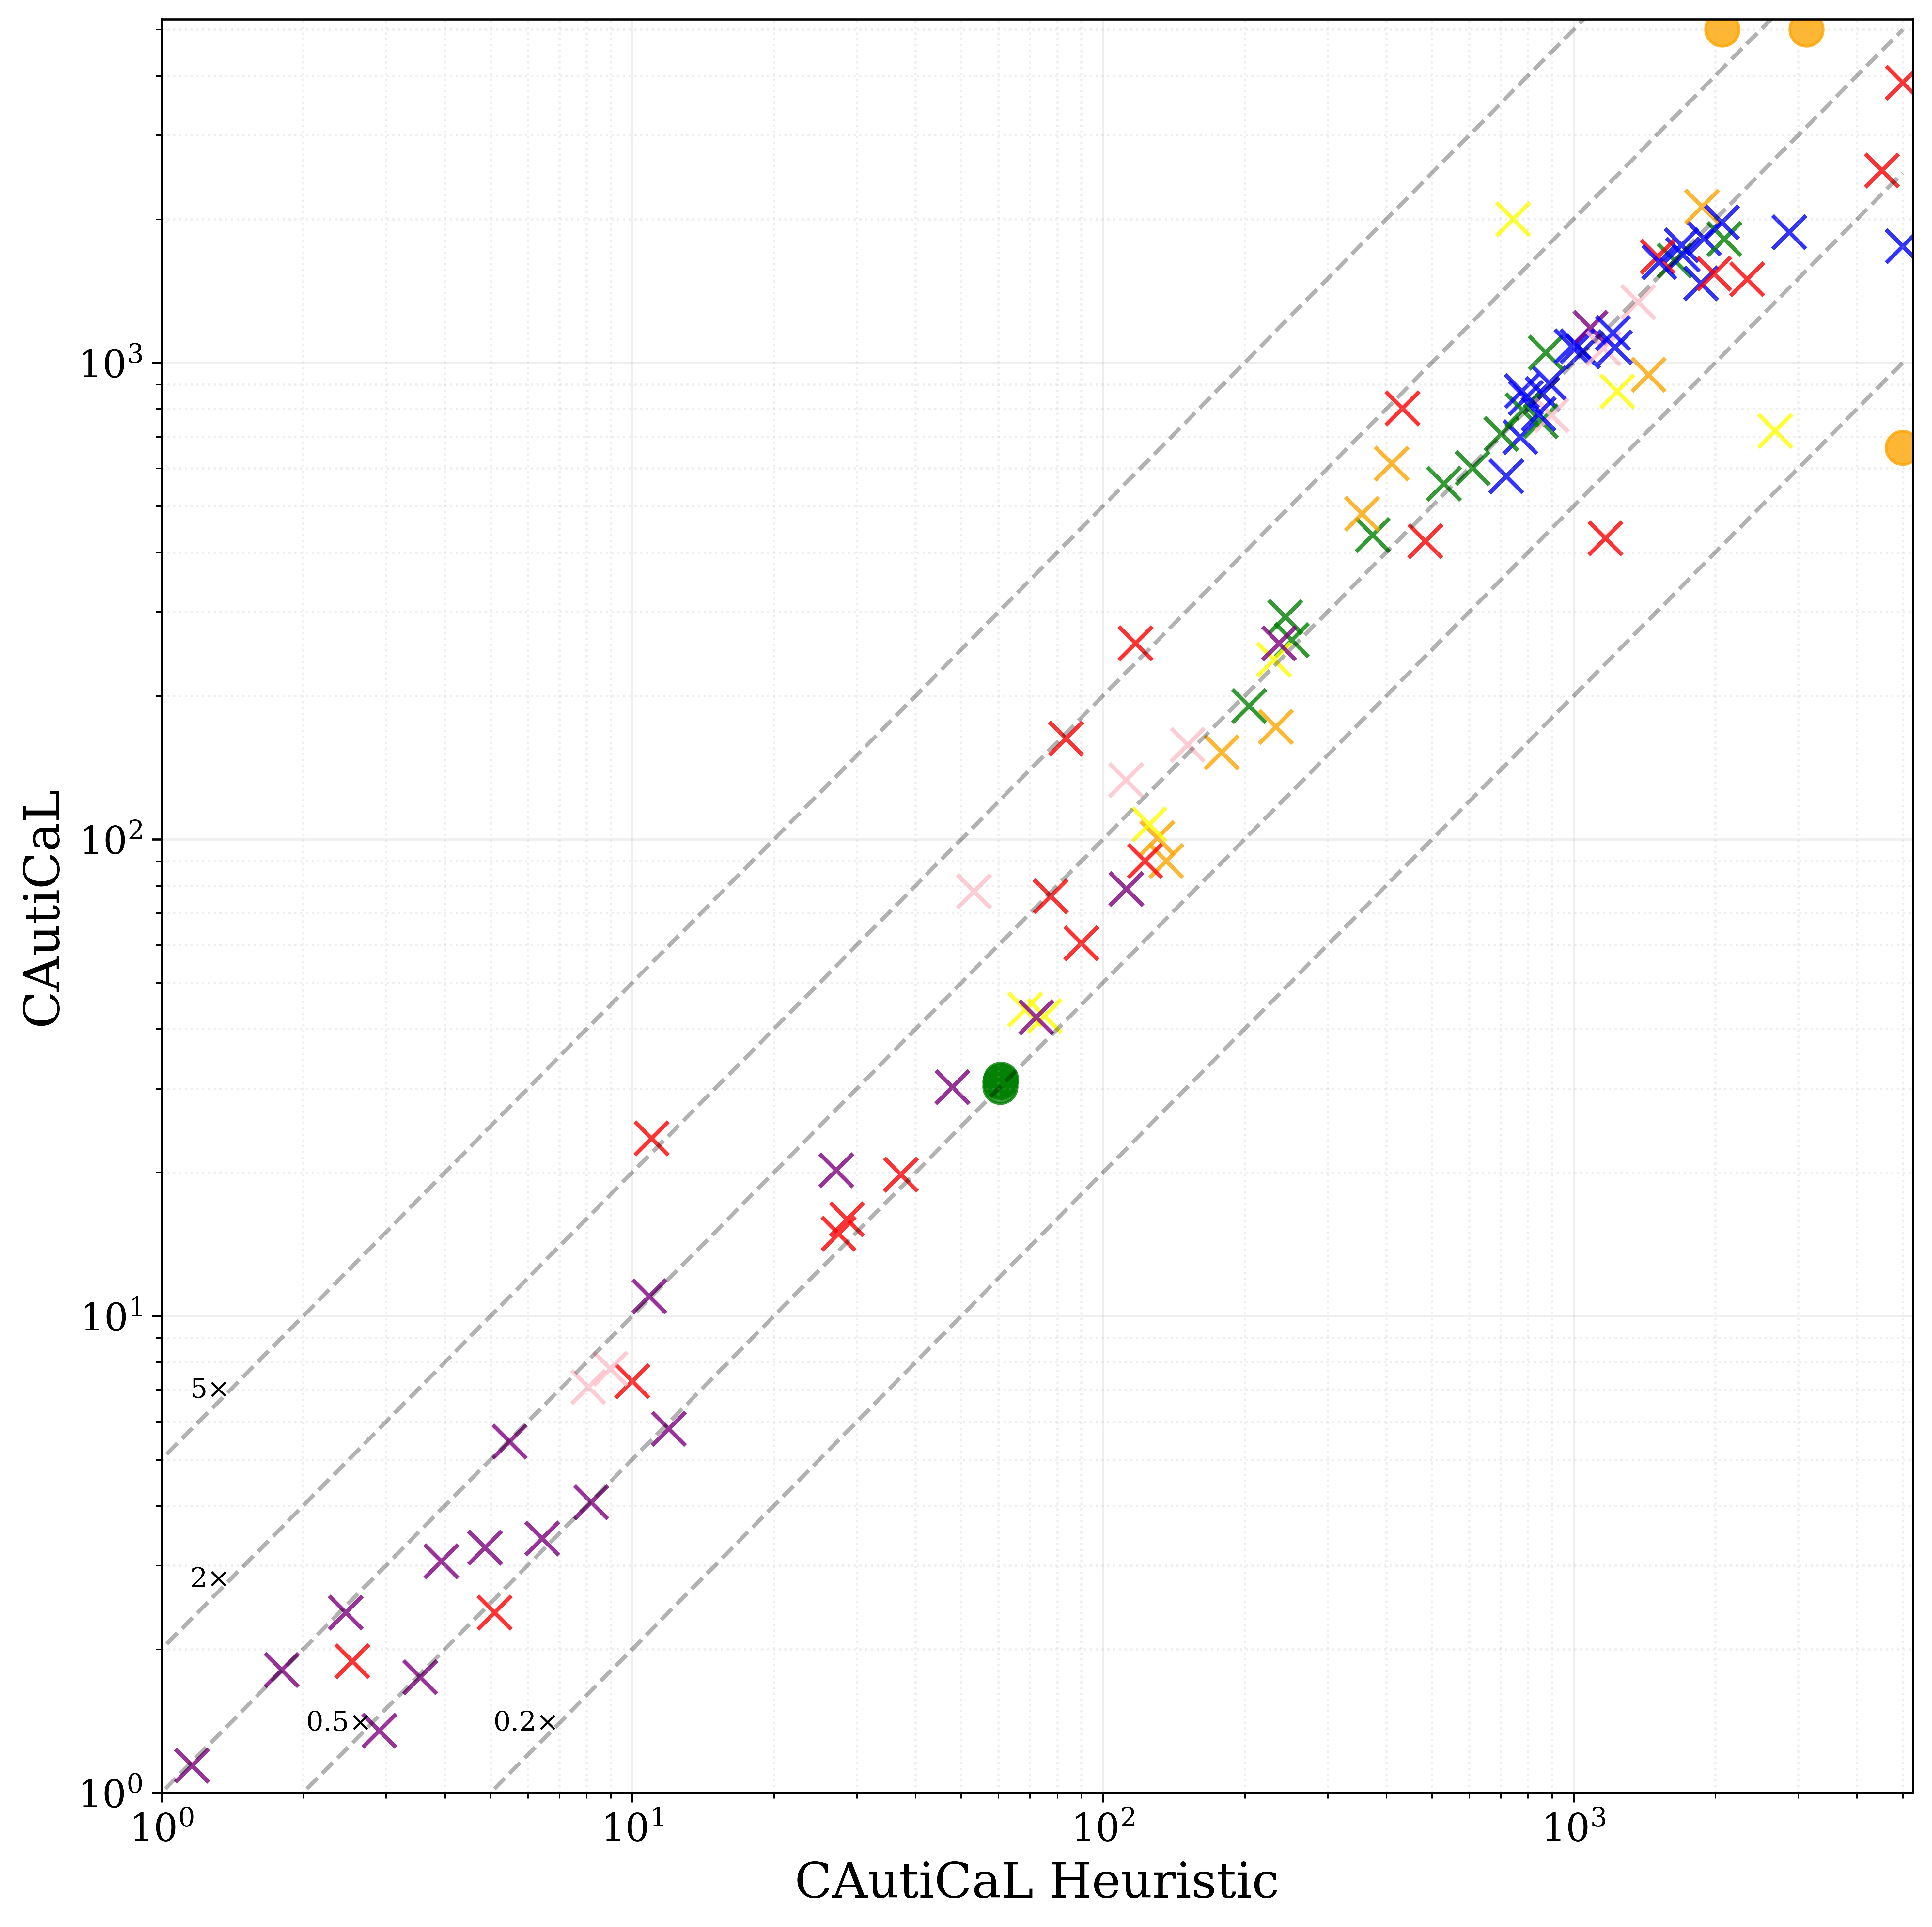
\includegraphics[width=\textwidth]{figs/globaldouble_heuristic_comparison.jpg}
            \caption{Double}
            \label{fig:cautical-vs-cadical}
    \end{subfigure}
        % \hspace{0.06\textwidth}
    % \hspace{0.06\textwidth}
    \begin{subfigure}[t]{0.3\textwidth}
        \centering
        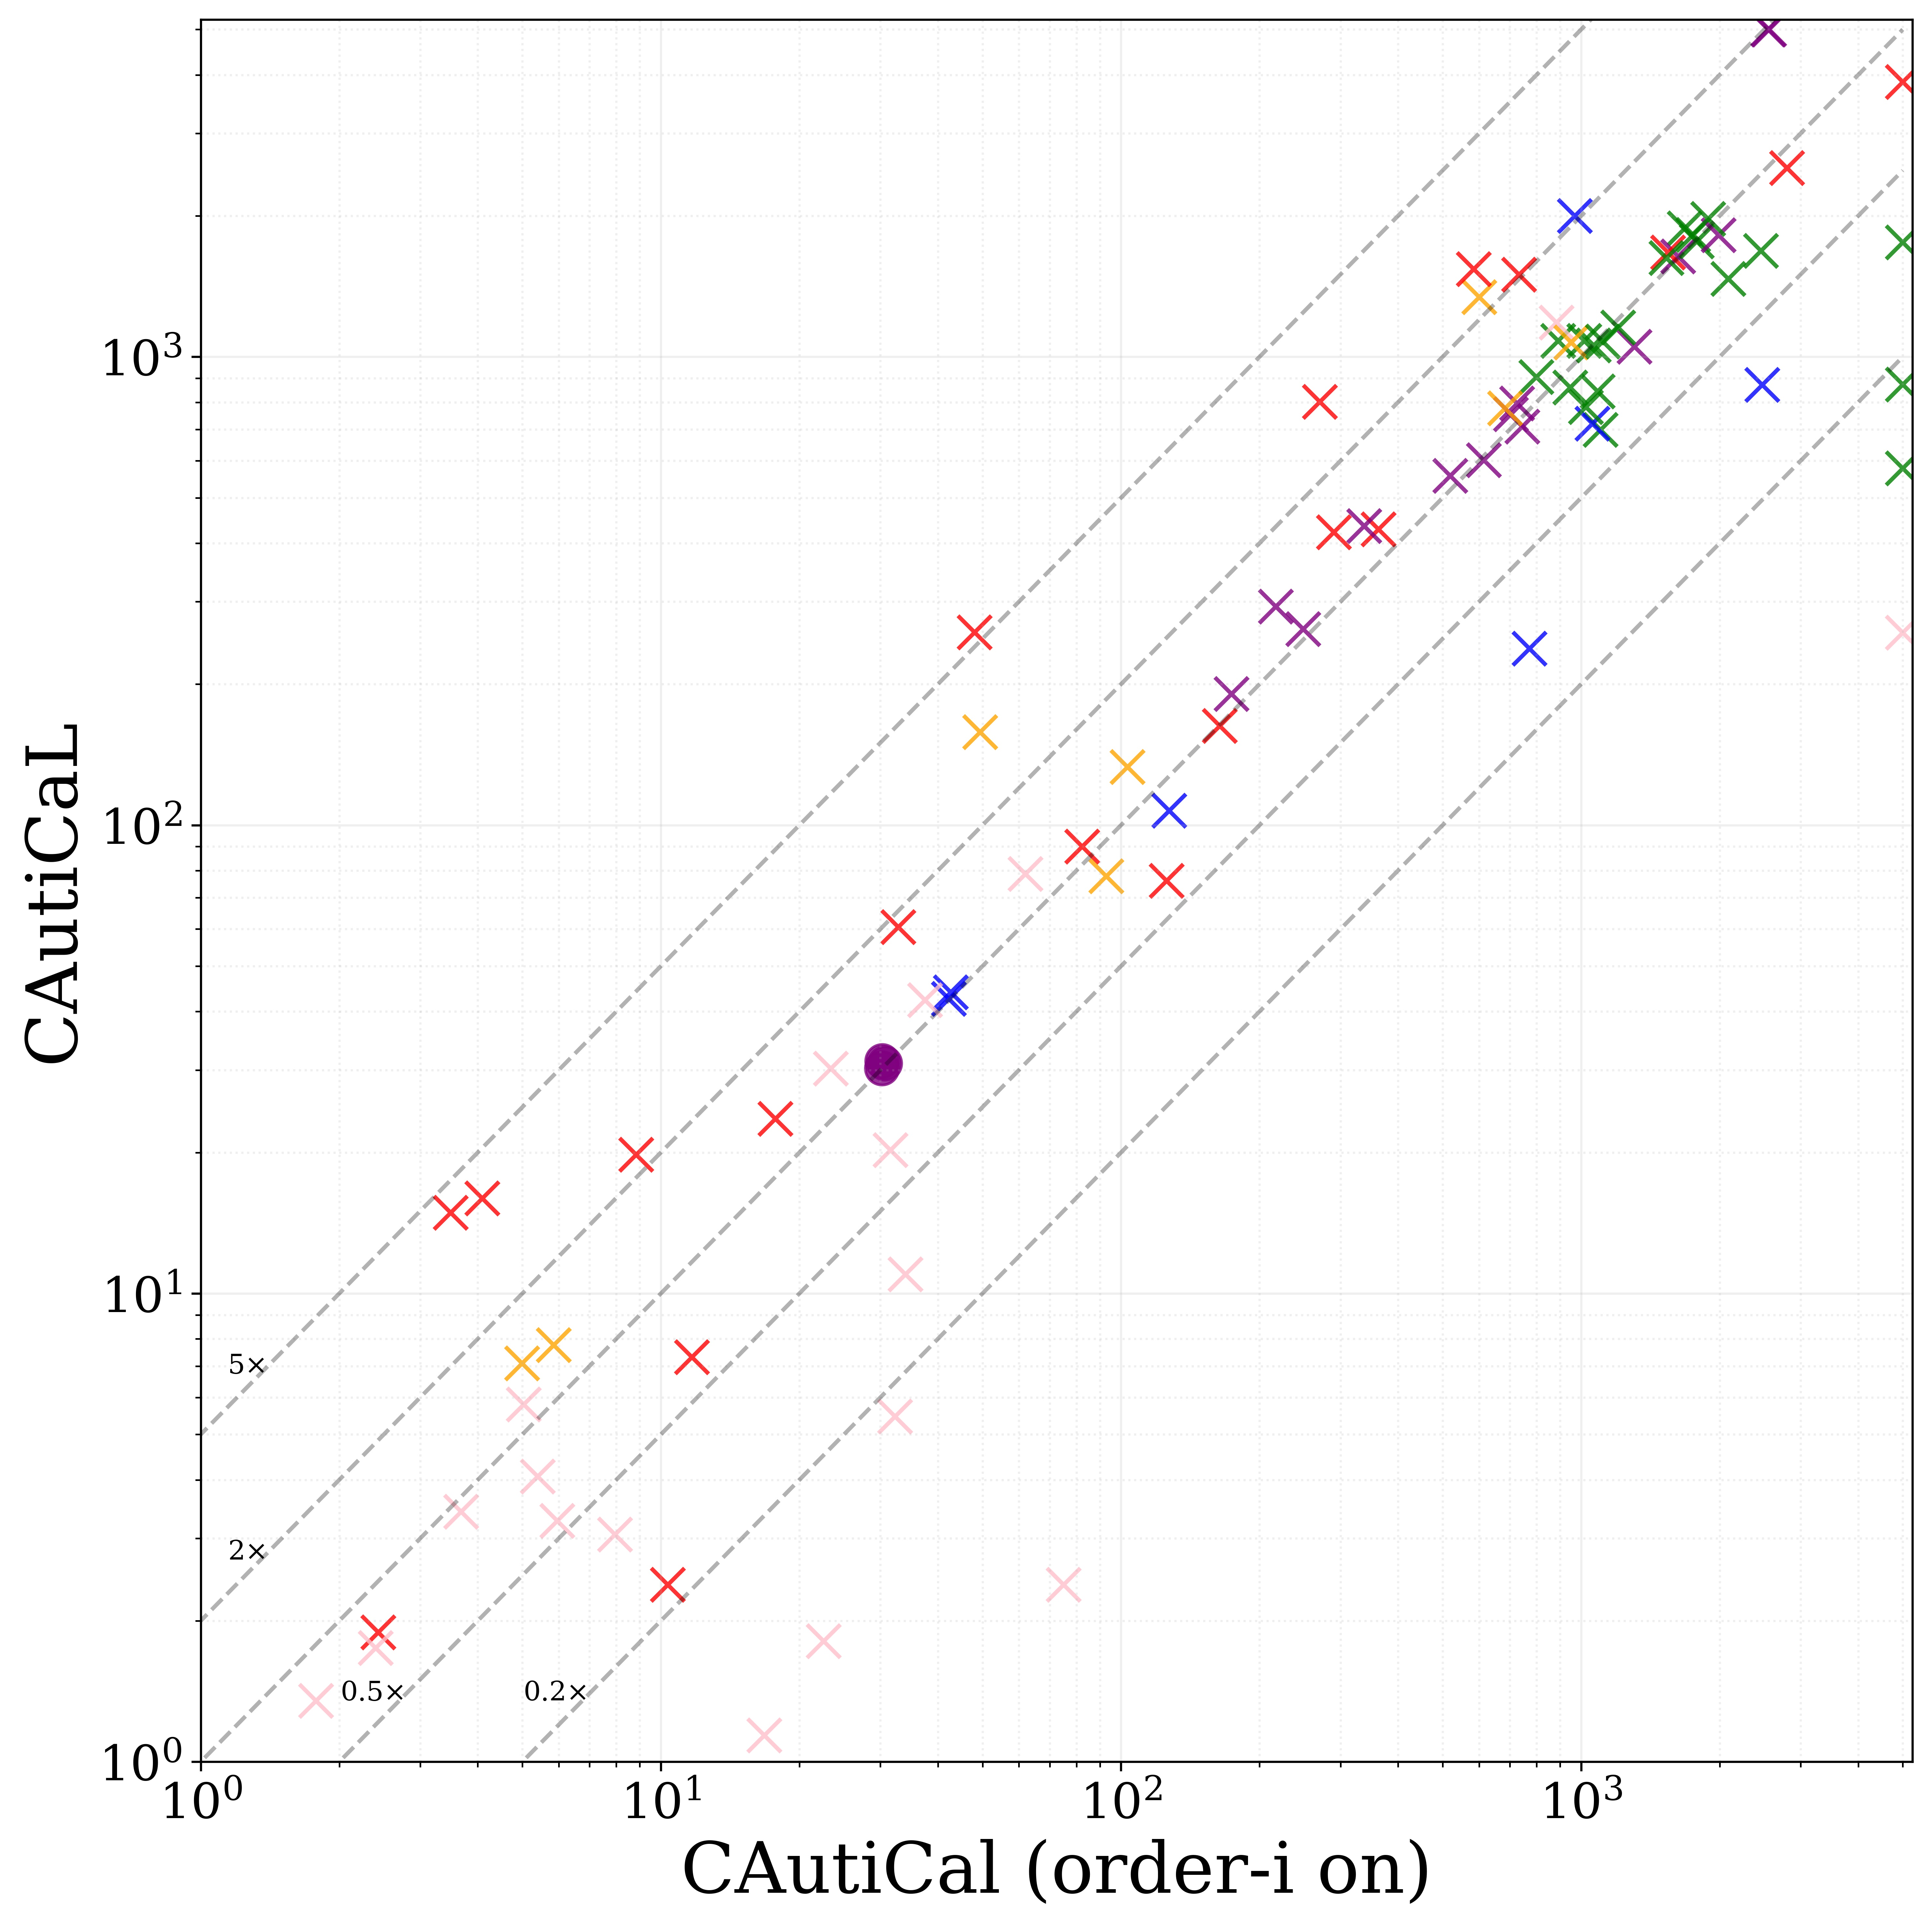
\includegraphics[width=\textwidth]{figs/globalisort_heuristic_comparison.jpg}
        \caption{Sort $i$ beforehand by frequency used}
        \label{fig:cautical-vs-prelearn}
    \end{subfigure}
    \begin{subfigure}[t]{0.3\textwidth}
        \centering
        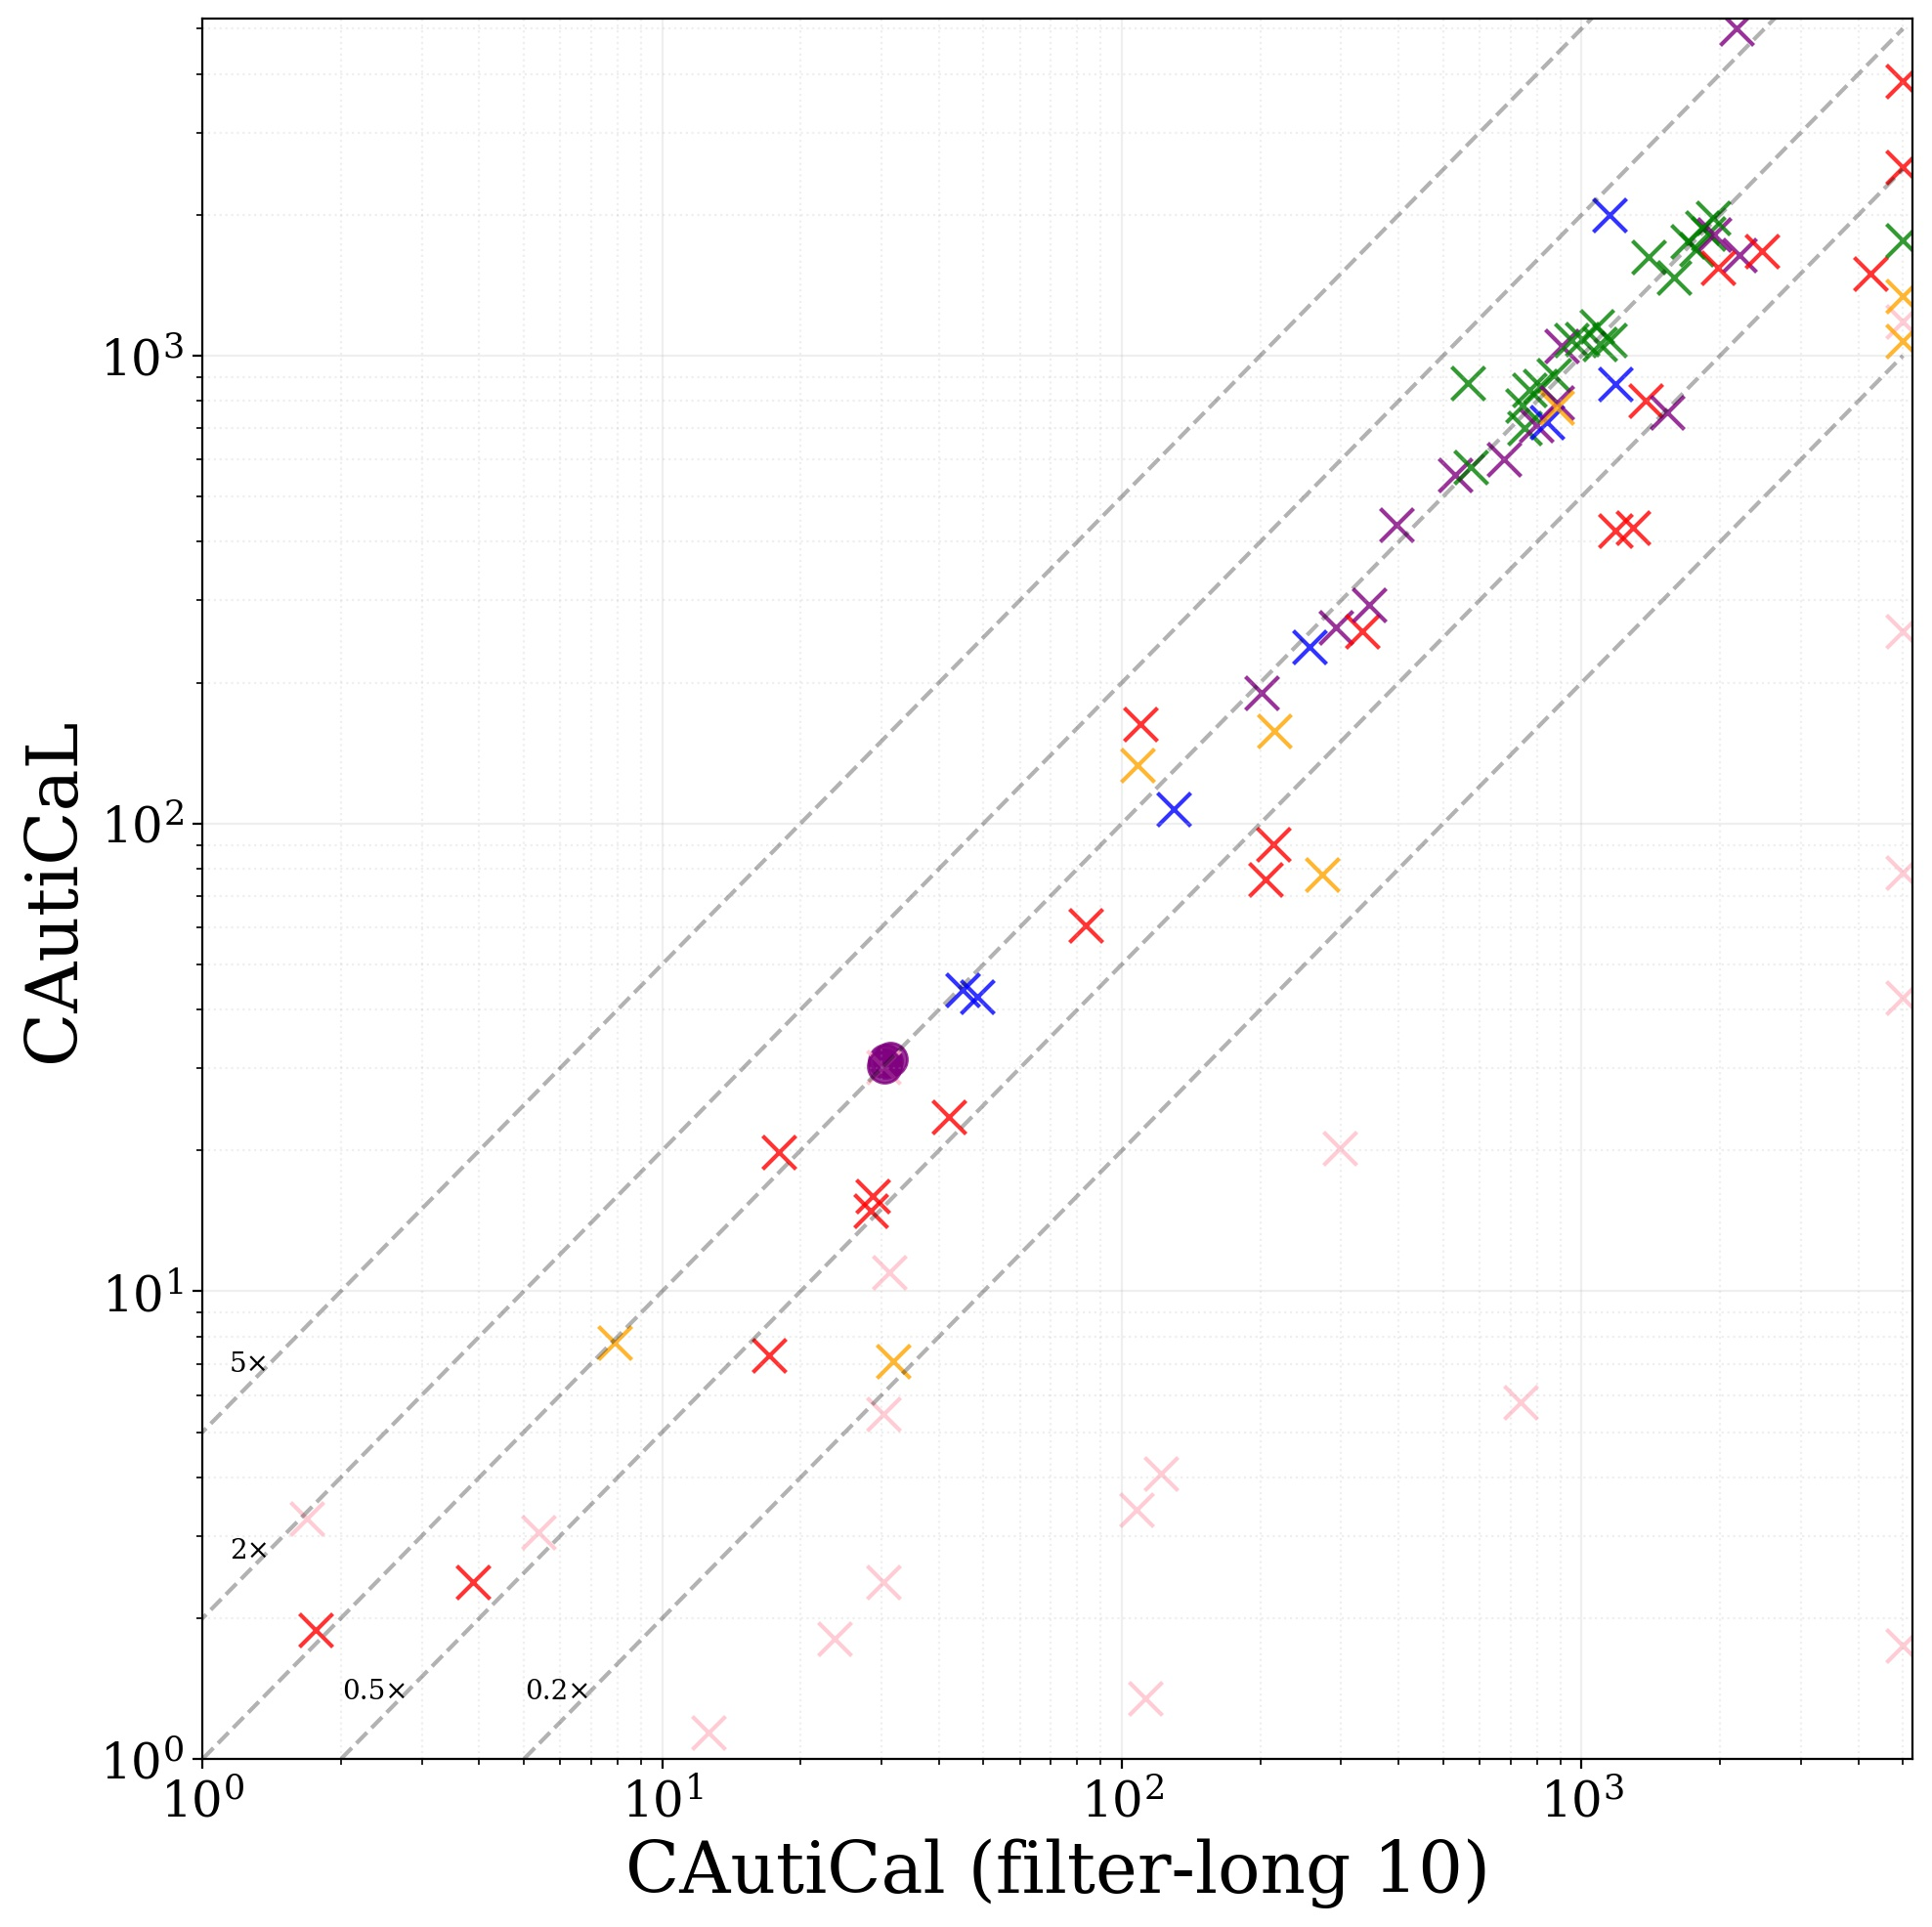
\includegraphics[width=\textwidth]{figs/globalmaxlen_heuristic_comparison.jpg}
        \caption{Max length}
        \label{fig:cautical-vs-prelearn}
    \end{subfigure}

    \caption{Performance comparison of \tool with other solvers}
    \label{fig:solver-comparison}
\end{figure*}

\begin{figure*}[!t]
    \centering
    \begin{subfigure}[t]{0.3\textwidth}
            \centering
            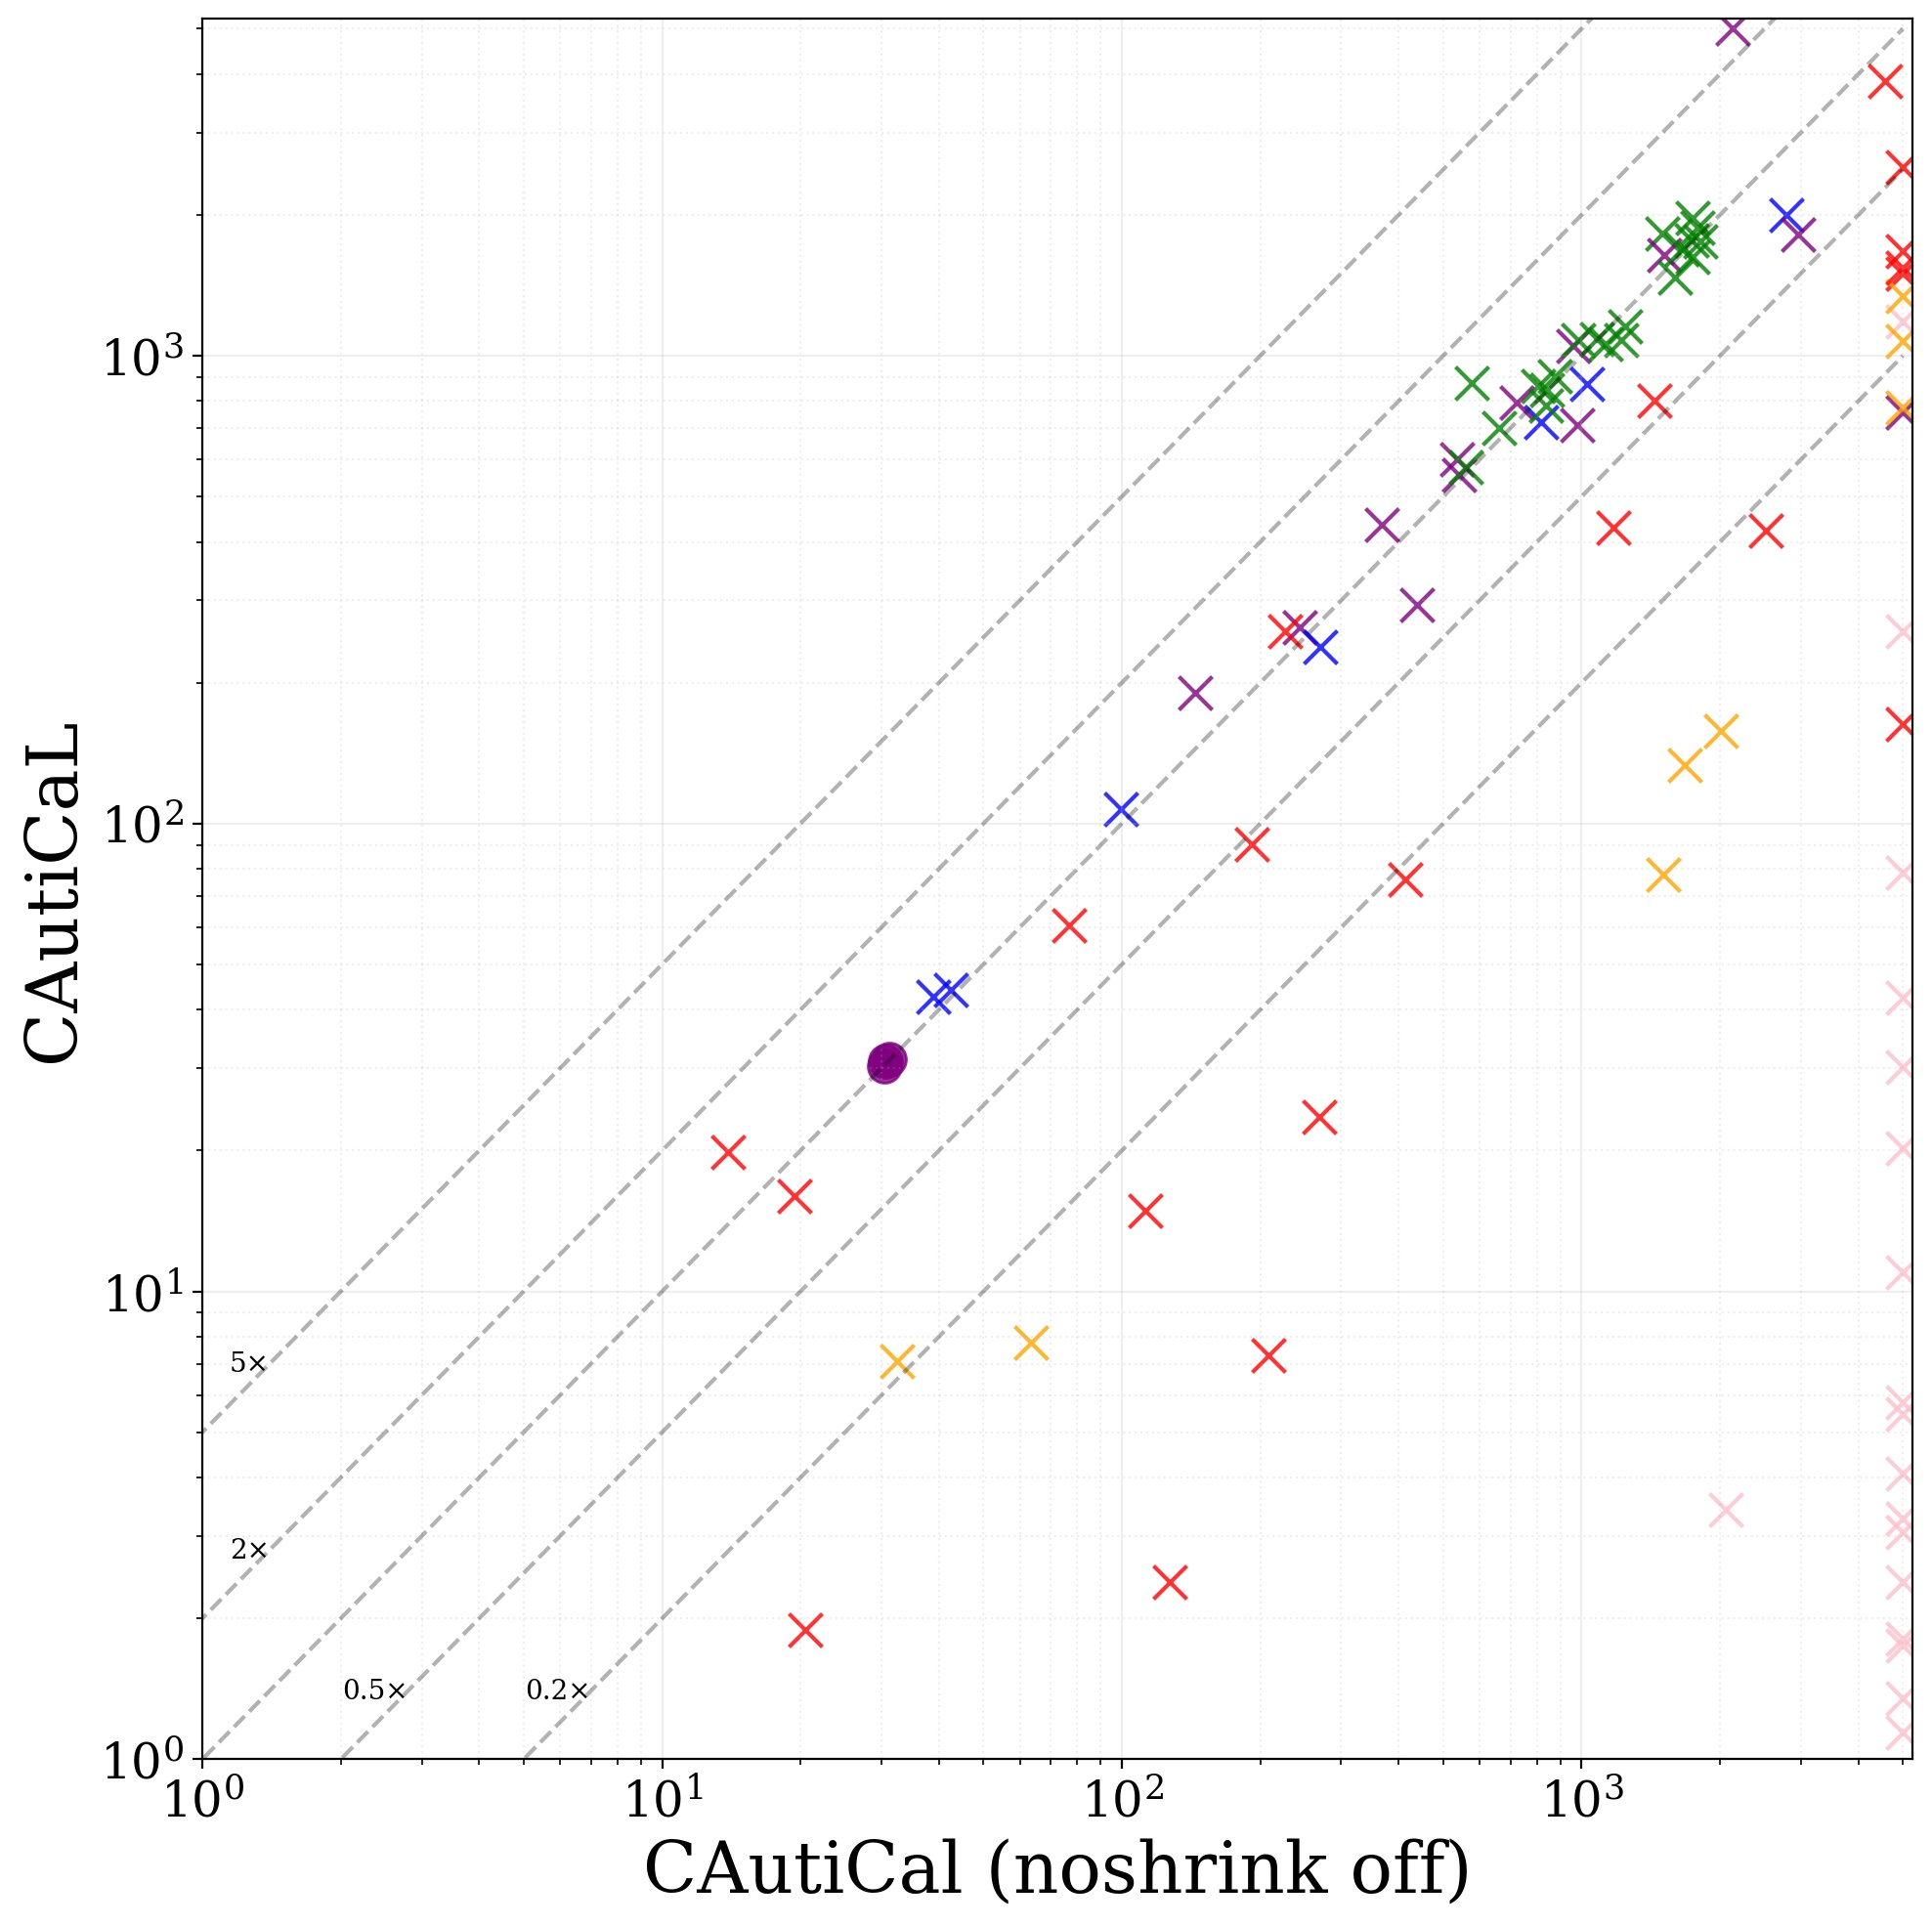
\includegraphics[width=\textwidth]{figs/globalnoshrink_heuristic_comparison.jpg}
            \caption{No shrink}
            \label{fig:cautical-vs-cadical}
    \end{subfigure}
        % \hspace{0.06\textwidth}
    % \hspace{0.06\textwidth}
    \begin{subfigure}[t]{0.3\textwidth}
        \centering
        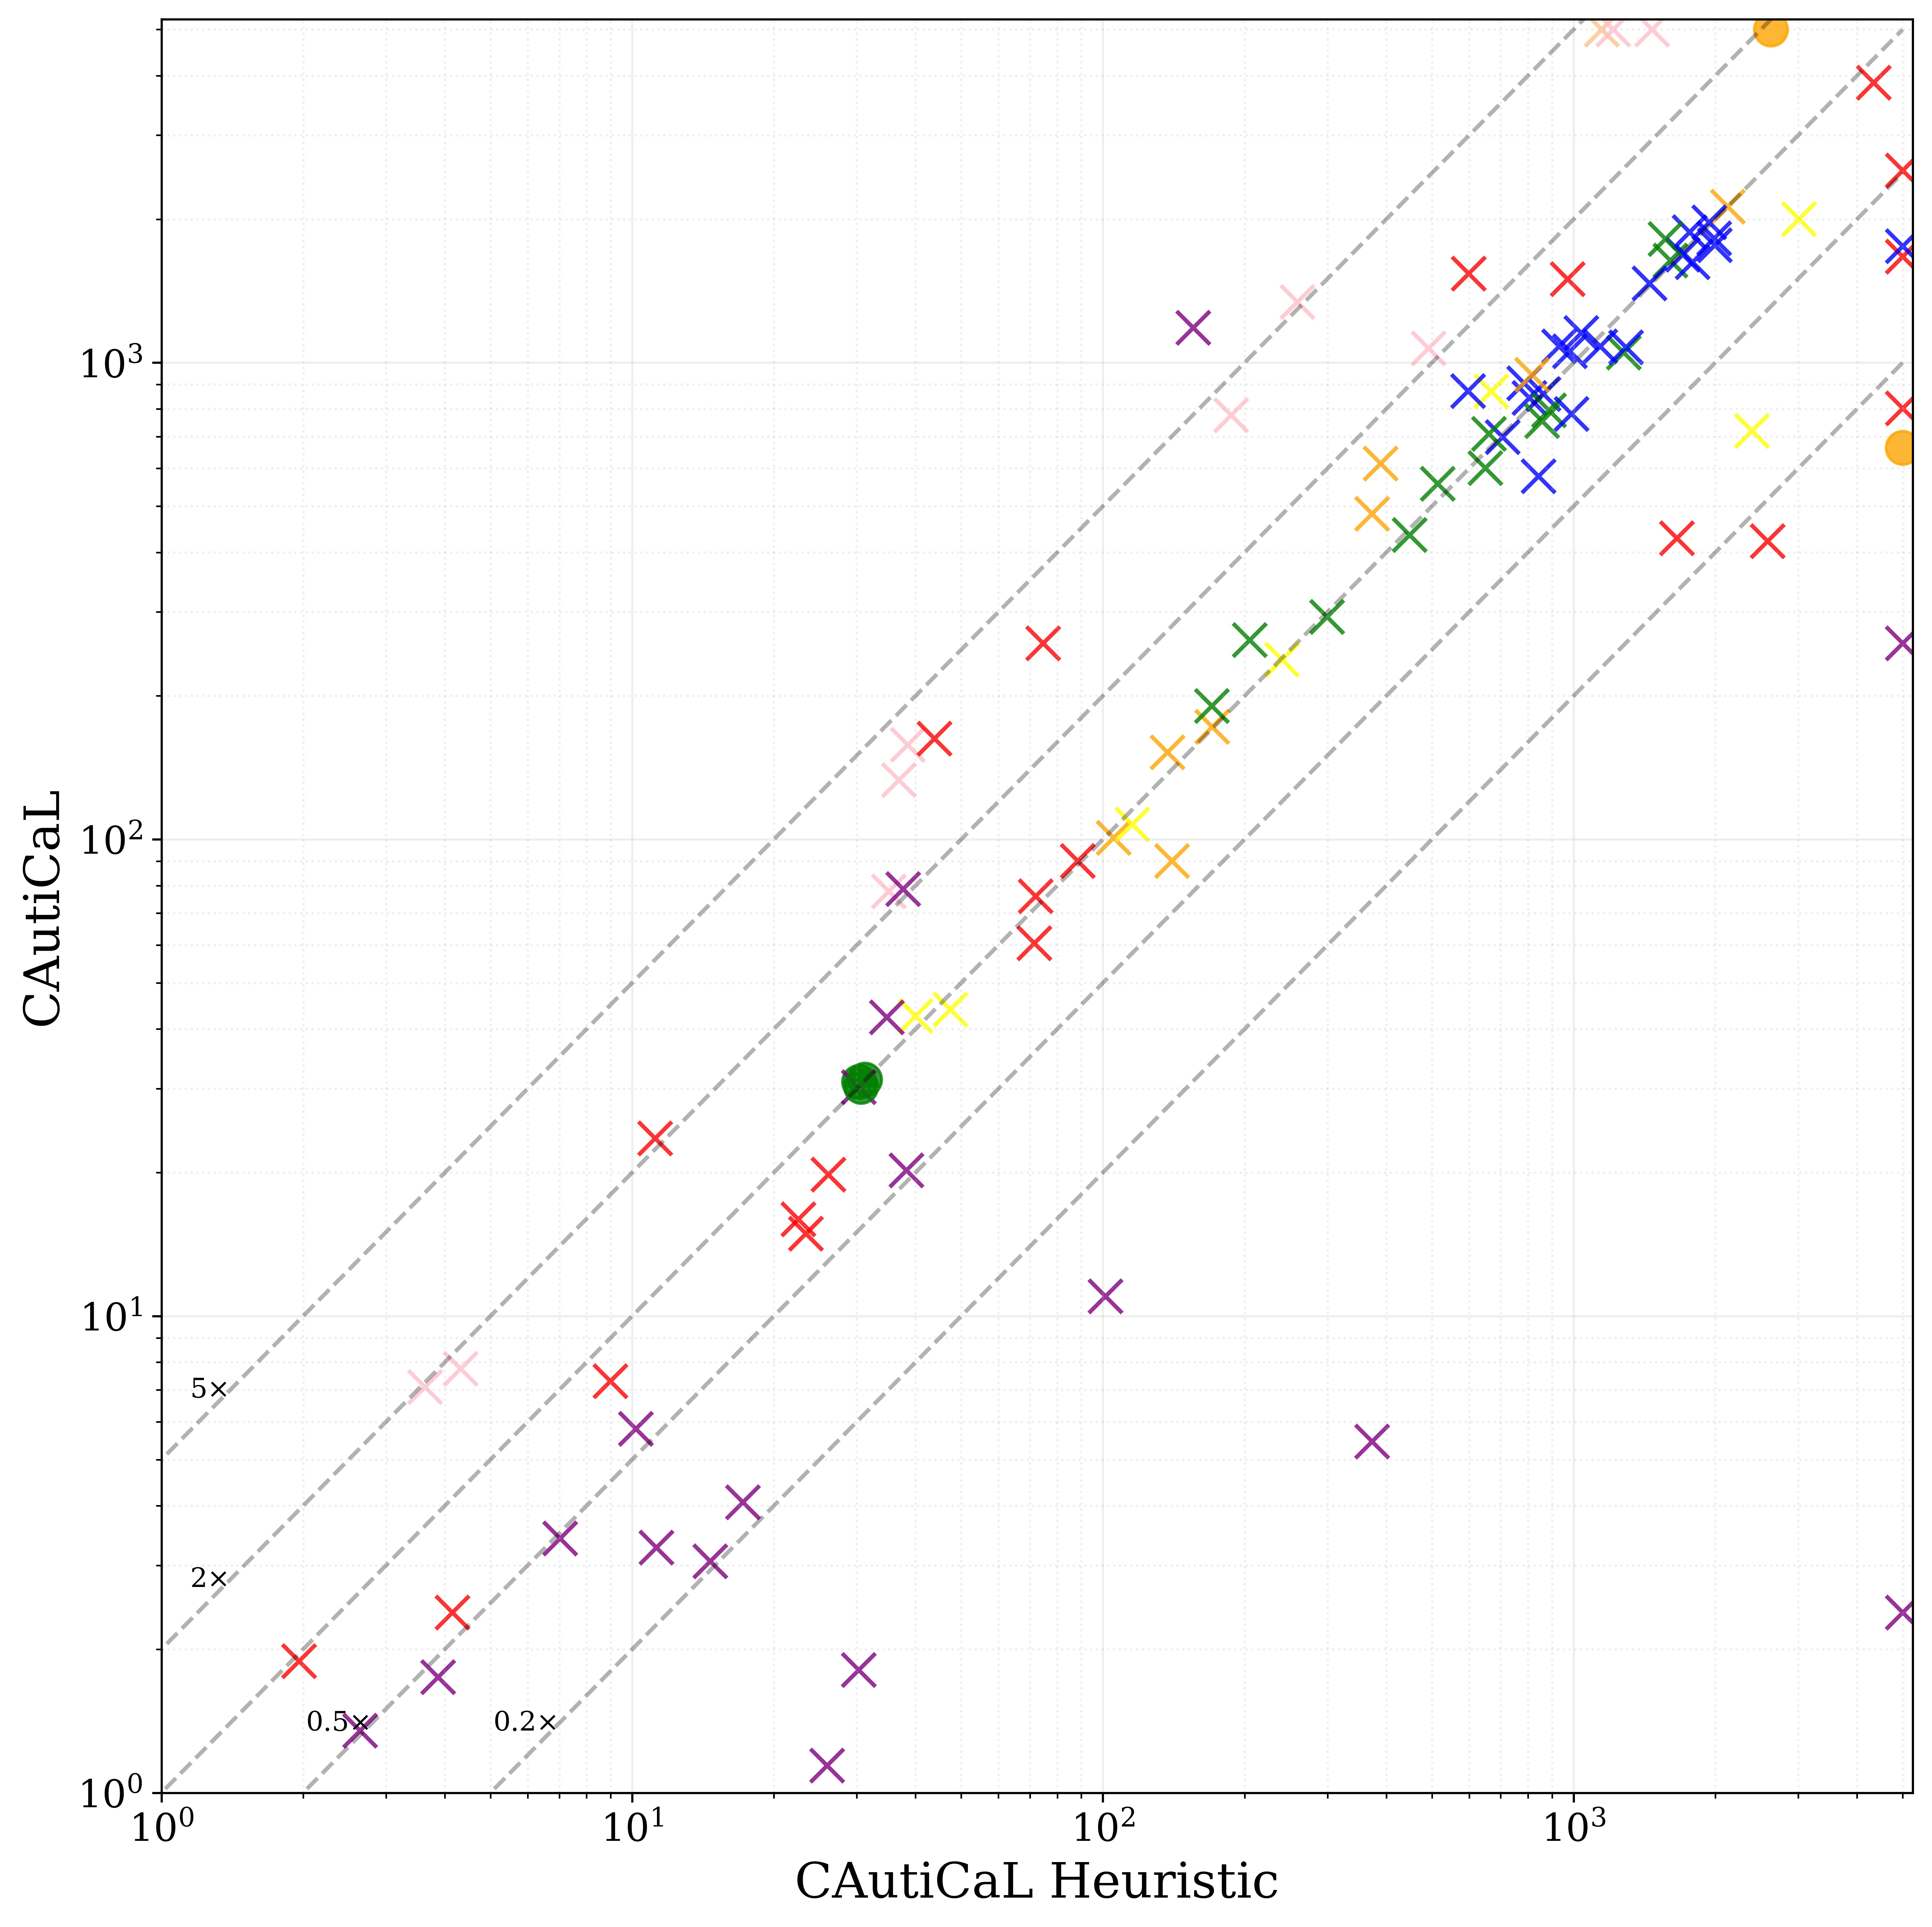
\includegraphics[width=\textwidth]{figs/globalorderi_heuristic_comparison.jpg}
        \caption{Order $i$ beforehand in increasing order}
        \label{fig:cautical-vs-prelearn}
    \end{subfigure}
    \begin{subfigure}[t]{0.3\textwidth}
        \centering
        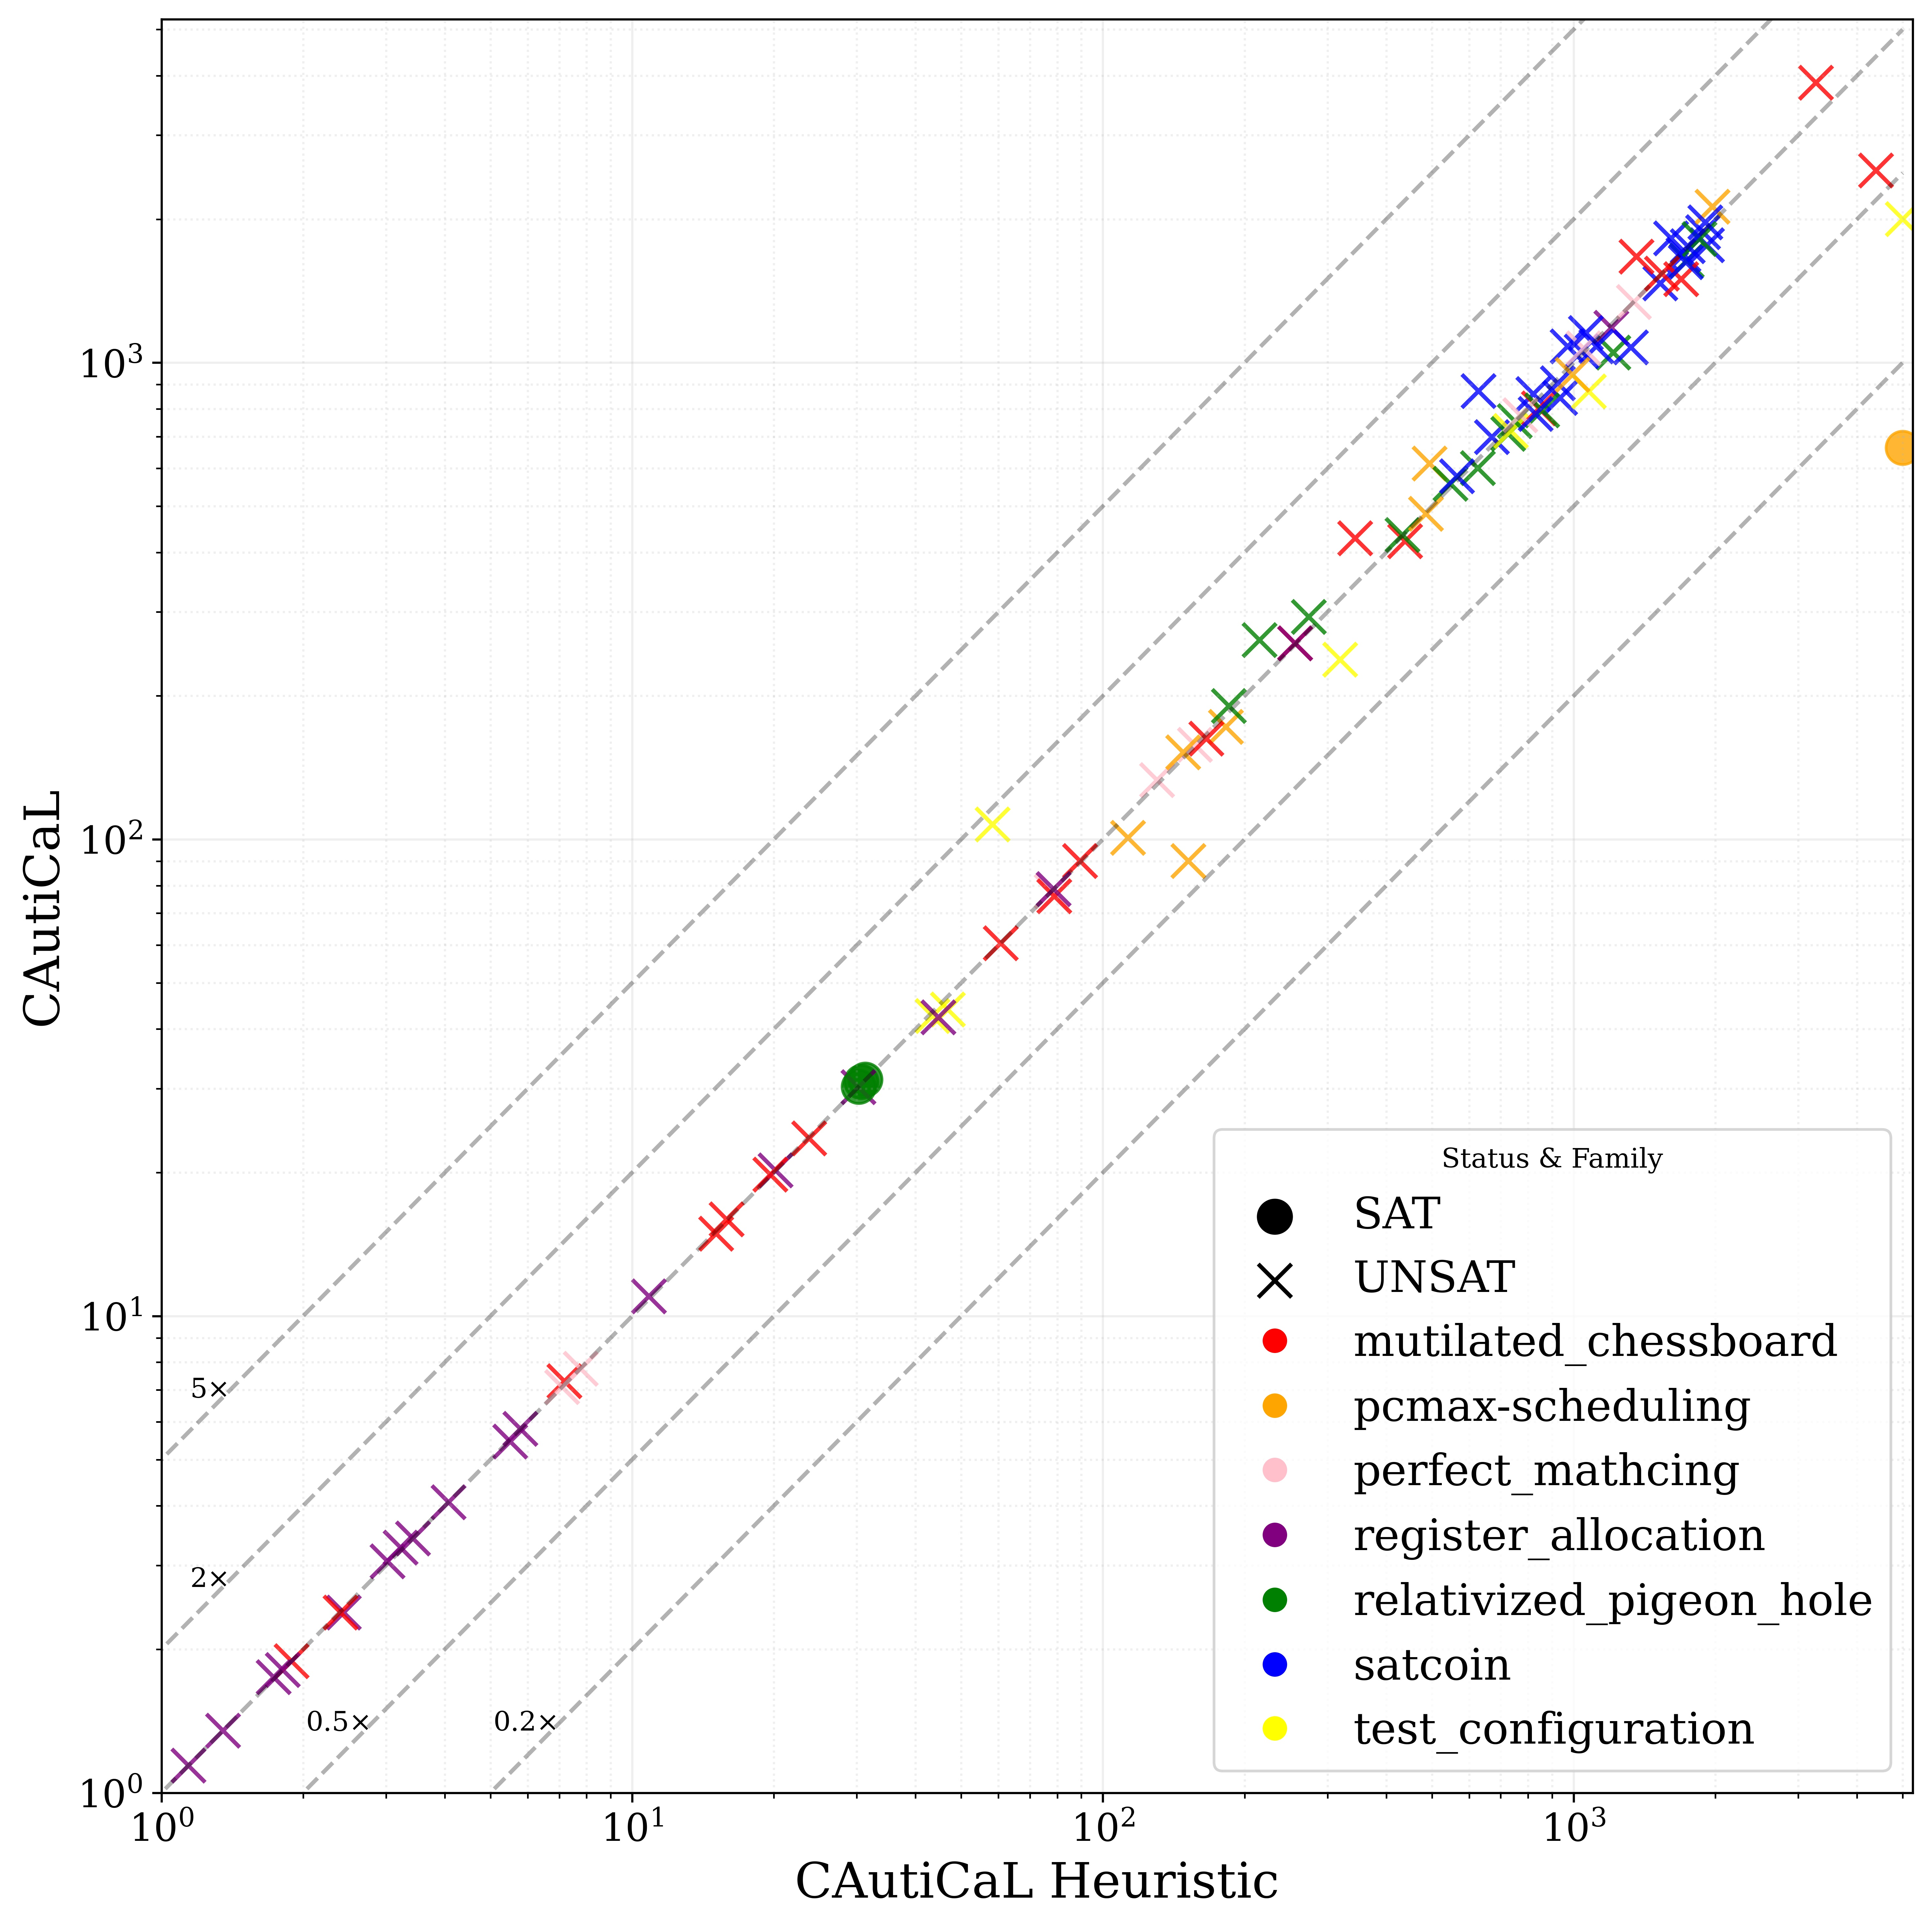
\includegraphics[width=\textwidth]{figs/globaltouch_heuristic_comparison.jpg}
        \caption{Touched heuristic}
        \label{fig:cautical-vs-prelearn}
    \end{subfigure}

    \caption{Performance comparison of \tool with other solvers}
    \label{fig:solver-comparison}
\end{figure*}


\subsection{Research Questions}~\label{subsec:eval-research-questions}

We answer the research questions posed at the start of this section. For
question 1, we conclude positively that \tool is able to provide short \pr
proofs for certain benchmark families. We match the best known result for The

However, it is currently unknown whether conditional autarkies can be used to
learn the shortest known \pr proofs for the mutilated
chessboard~\cite{mutilatedchessboard-pr} or Tseitin graph
formulas~\cite{sadical}. Additionally, there are benchmarks in the ??, ??, and
?? families that \prelearn solves and \tool does not.

For question 2, we can conclude positively that \tool is less sensitive to
encoding choices compared to other \pr learning techniques. We show that \tool
has $O(n^3)$ proofs for the pigeonhole principle even when the variables are
permuted, clauses are permuted, and literals are flipped. Additionally, \tool
does not consider any information about the encoding when propagating literals
(it does so randomly). In fact, we show that heuristics used to rank order
literals have an adverse effect on performance.